% Options for packages loaded elsewhere
\PassOptionsToPackage{unicode}{hyperref}
\PassOptionsToPackage{hyphens}{url}
%
\documentclass[
  12pt]{article}
\usepackage{amsmath,amssymb}
\usepackage{lmodern}
\usepackage{iftex}
\ifPDFTeX
  \usepackage[T1]{fontenc}
  \usepackage[utf8]{inputenc}
  \usepackage{textcomp} % provide euro and other symbols
\else % if luatex or xetex
  \usepackage{unicode-math}
  \defaultfontfeatures{Scale=MatchLowercase}
  \defaultfontfeatures[\rmfamily]{Ligatures=TeX,Scale=1}
  \setmainfont[]{Arial}
\fi
% Use upquote if available, for straight quotes in verbatim environments
\IfFileExists{upquote.sty}{\usepackage{upquote}}{}
\IfFileExists{microtype.sty}{% use microtype if available
  \usepackage[]{microtype}
  \UseMicrotypeSet[protrusion]{basicmath} % disable protrusion for tt fonts
}{}
\makeatletter
\@ifundefined{KOMAClassName}{% if non-KOMA class
  \IfFileExists{parskip.sty}{%
    \usepackage{parskip}
  }{% else
    \setlength{\parindent}{0pt}
    \setlength{\parskip}{6pt plus 2pt minus 1pt}}
}{% if KOMA class
  \KOMAoptions{parskip=half}}
\makeatother
\usepackage{xcolor}
\IfFileExists{xurl.sty}{\usepackage{xurl}}{} % add URL line breaks if available
\IfFileExists{bookmark.sty}{\usepackage{bookmark}}{\usepackage{hyperref}}
\hypersetup{
  pdftitle={Guide to the Cumulative CES Policy Preferences},
  pdfauthor={Angelo Dagonel},
  hidelinks,
  pdfcreator={LaTeX via pandoc}}
\urlstyle{same} % disable monospaced font for URLs
\usepackage[margin=3cm]{geometry}
\usepackage{color}
\usepackage{fancyvrb}
\newcommand{\VerbBar}{|}
\newcommand{\VERB}{\Verb[commandchars=\\\{\}]}
\DefineVerbatimEnvironment{Highlighting}{Verbatim}{commandchars=\\\{\}}
% Add ',fontsize=\small' for more characters per line
\usepackage{framed}
\definecolor{shadecolor}{RGB}{248,248,248}
\newenvironment{Shaded}{\begin{snugshade}}{\end{snugshade}}
\newcommand{\AlertTok}[1]{\textcolor[rgb]{0.94,0.16,0.16}{#1}}
\newcommand{\AnnotationTok}[1]{\textcolor[rgb]{0.56,0.35,0.01}{\textbf{\textit{#1}}}}
\newcommand{\AttributeTok}[1]{\textcolor[rgb]{0.77,0.63,0.00}{#1}}
\newcommand{\BaseNTok}[1]{\textcolor[rgb]{0.00,0.00,0.81}{#1}}
\newcommand{\BuiltInTok}[1]{#1}
\newcommand{\CharTok}[1]{\textcolor[rgb]{0.31,0.60,0.02}{#1}}
\newcommand{\CommentTok}[1]{\textcolor[rgb]{0.56,0.35,0.01}{\textit{#1}}}
\newcommand{\CommentVarTok}[1]{\textcolor[rgb]{0.56,0.35,0.01}{\textbf{\textit{#1}}}}
\newcommand{\ConstantTok}[1]{\textcolor[rgb]{0.00,0.00,0.00}{#1}}
\newcommand{\ControlFlowTok}[1]{\textcolor[rgb]{0.13,0.29,0.53}{\textbf{#1}}}
\newcommand{\DataTypeTok}[1]{\textcolor[rgb]{0.13,0.29,0.53}{#1}}
\newcommand{\DecValTok}[1]{\textcolor[rgb]{0.00,0.00,0.81}{#1}}
\newcommand{\DocumentationTok}[1]{\textcolor[rgb]{0.56,0.35,0.01}{\textbf{\textit{#1}}}}
\newcommand{\ErrorTok}[1]{\textcolor[rgb]{0.64,0.00,0.00}{\textbf{#1}}}
\newcommand{\ExtensionTok}[1]{#1}
\newcommand{\FloatTok}[1]{\textcolor[rgb]{0.00,0.00,0.81}{#1}}
\newcommand{\FunctionTok}[1]{\textcolor[rgb]{0.00,0.00,0.00}{#1}}
\newcommand{\ImportTok}[1]{#1}
\newcommand{\InformationTok}[1]{\textcolor[rgb]{0.56,0.35,0.01}{\textbf{\textit{#1}}}}
\newcommand{\KeywordTok}[1]{\textcolor[rgb]{0.13,0.29,0.53}{\textbf{#1}}}
\newcommand{\NormalTok}[1]{#1}
\newcommand{\OperatorTok}[1]{\textcolor[rgb]{0.81,0.36,0.00}{\textbf{#1}}}
\newcommand{\OtherTok}[1]{\textcolor[rgb]{0.56,0.35,0.01}{#1}}
\newcommand{\PreprocessorTok}[1]{\textcolor[rgb]{0.56,0.35,0.01}{\textit{#1}}}
\newcommand{\RegionMarkerTok}[1]{#1}
\newcommand{\SpecialCharTok}[1]{\textcolor[rgb]{0.00,0.00,0.00}{#1}}
\newcommand{\SpecialStringTok}[1]{\textcolor[rgb]{0.31,0.60,0.02}{#1}}
\newcommand{\StringTok}[1]{\textcolor[rgb]{0.31,0.60,0.02}{#1}}
\newcommand{\VariableTok}[1]{\textcolor[rgb]{0.00,0.00,0.00}{#1}}
\newcommand{\VerbatimStringTok}[1]{\textcolor[rgb]{0.31,0.60,0.02}{#1}}
\newcommand{\WarningTok}[1]{\textcolor[rgb]{0.56,0.35,0.01}{\textbf{\textit{#1}}}}
\usepackage{graphicx}
\makeatletter
\def\maxwidth{\ifdim\Gin@nat@width>\linewidth\linewidth\else\Gin@nat@width\fi}
\def\maxheight{\ifdim\Gin@nat@height>\textheight\textheight\else\Gin@nat@height\fi}
\makeatother
% Scale images if necessary, so that they will not overflow the page
% margins by default, and it is still possible to overwrite the defaults
% using explicit options in \includegraphics[width, height, ...]{}
\setkeys{Gin}{width=\maxwidth,height=\maxheight,keepaspectratio}
% Set default figure placement to htbp
\makeatletter
\def\fps@figure{htbp}
\makeatother
\setlength{\emergencystretch}{3em} % prevent overfull lines
\providecommand{\tightlist}{%
  \setlength{\itemsep}{0pt}\setlength{\parskip}{0pt}}
\setcounter{secnumdepth}{5}
\usepackage{dcolumn}\usepackage{setspace}\singlespacing\usepackage{graphicx}\usepackage{caption}\captionsetup[table]{skip=10pt}\hypersetup{colorlinks=true,urlcolor=blue,linkcolor=black}
\usepackage{booktabs}
\usepackage{longtable}
\usepackage{array}
\usepackage{multirow}
\usepackage{wrapfig}
\usepackage{float}
\usepackage{colortbl}
\usepackage{pdflscape}
\usepackage{tabu}
\usepackage{threeparttable}
\usepackage{threeparttablex}
\usepackage[normalem]{ulem}
\usepackage{makecell}
\usepackage{xcolor}
\ifLuaTeX
  \usepackage{selnolig}  % disable illegal ligatures
\fi

\title{\Large Guide to the Cumulative CES Policy Preferences}
\author{Angelo Dagonel\footnote{PhD candidate, Department of Government,
  Harvard University. Thanks to Shiro Kuriwaki, Stephen Ansolabehere and
  Brian Schaffner for their suggestions and guidance. Please send bug
  reports to \url{dagonel@g.harvard.edu}, or the
  \href{https://github.com/psjello/cumulative_cces_policy_preferences}{Github
  repository} for the guide.}}
\date{Guide last updated: 2022-09-06}

\begin{document}
\maketitle

\begin{quote}
Dagonel, Angelo, 2022, ``Cumulative CES Policy Preferences'',
\href{https://dataverse.harvard.edu/dataset.xhtml?persistentId=doi:10.7910/DVN/OSXDQO}{\url{doi:10.7910/DVN/OSXDQO}},
Harvard Dataverse, V2.
\end{quote}

\bigskip

Each year, the Cooperative Election Study (CES)\footnote{Formerly the
  Cooperative Congressional Election Study (CCES).} asks respondents
about their preferences on issues like abortion, immigration, the
environment and more. However, variable names for question items often
change from year to year.

\medskip

The \textbf{Cumulative CES Policy Preferences} data set compiles various
policy preference question items from CES respondents over time. This
represents an effort to track, rename, recode, and append together
557,456 responses across 54 policy preference question items from 16
individual CES survey data sets, ranging from 2006 to 2021.

\medskip

The resulting time series is available as a
\href{https://dataverse.harvard.edu/dataset.xhtml?persistentId=doi:10.7910/DVN/OSXDQO}{downloadable
data set from the Harvard Dataverse}. This data set can be combined with
the geographic, demographic, and political characteristics of each
respondent from the
\href{https://dataverse.harvard.edu/dataset.xhtml?persistentId=doi:10.7910/DVN/II2DB6}{Cumulative
CES Common Content} by merging on the \texttt{case\_id} and
\texttt{year} variables.

\medskip

Question items are categorized into nine issue area categories. Variable
names include the issue category, and a suffix related to the specific
question. Variable labels contain a condensed, one sentence description
of the policy that respondents are being asked if they support or
oppose. For each question item, this guide provides details on the years
where the item appears, frequency tables for response values, and it's
original, year-specific variable name and question wording.

\newpage

\hypertarget{question-availability-by-year}{%
\section{Question availability by
year}\label{question-availability-by-year}}

\begin{table}[H]
\centering
\resizebox{\linewidth}{!}{
\begin{tabular}{lcccccccccccccccc}
\toprule
Common variable name & 2006 & 2007 & 2008 & 2009 & 2010 & 2011 & 2012 & 2013 & 2014 & 2015 & 2016 & 2017 & 2018 & 2019 & 2020 & 2021\\
\midrule
\cellcolor{gray!6}{case\_id} & \cellcolor{gray!6}{$\checkmark$} & \cellcolor{gray!6}{$\checkmark$} & \cellcolor{gray!6}{$\checkmark$} & \cellcolor{gray!6}{$\checkmark$} & \cellcolor{gray!6}{$\checkmark$} & \cellcolor{gray!6}{$\checkmark$} & \cellcolor{gray!6}{$\checkmark$} & \cellcolor{gray!6}{$\checkmark$} & \cellcolor{gray!6}{$\checkmark$} & \cellcolor{gray!6}{$\checkmark$} & \cellcolor{gray!6}{$\checkmark$} & \cellcolor{gray!6}{$\checkmark$} & \cellcolor{gray!6}{$\checkmark$} & \cellcolor{gray!6}{$\checkmark$} & \cellcolor{gray!6}{$\checkmark$} & \cellcolor{gray!6}{$\checkmark$}\\
$\textbf{Abortion}$ &  &  &  &  &  &  &  &  &  &  &  &  &  &  &  & \\
\cellcolor{gray!6}{$\hspace{10pt}$abortion\_scale} & \cellcolor{gray!6}{$\checkmark$} & \cellcolor{gray!6}{$\checkmark$} & \cellcolor{gray!6}{$\checkmark$} & \cellcolor{gray!6}{$\checkmark$} & \cellcolor{gray!6}{$\checkmark$} & \cellcolor{gray!6}{$\checkmark$} & \cellcolor{gray!6}{$\checkmark$} & \cellcolor{gray!6}{$\checkmark$} & \cellcolor{gray!6}{} & \cellcolor{gray!6}{} & \cellcolor{gray!6}{} & \cellcolor{gray!6}{} & \cellcolor{gray!6}{} & \cellcolor{gray!6}{} & \cellcolor{gray!6}{} & \cellcolor{gray!6}{}\\
$\hspace{10pt}$abortion\_always &  &  &  &  &  &  &  &  & $\checkmark$ & $\checkmark$ & $\checkmark$ & $\checkmark$ & $\checkmark$ & $\checkmark$ & $\checkmark$ & $\checkmark$\\
\cellcolor{gray!6}{$\hspace{10pt}$abortion\_conditional} & \cellcolor{gray!6}{} & \cellcolor{gray!6}{} & \cellcolor{gray!6}{} & \cellcolor{gray!6}{} & \cellcolor{gray!6}{} & \cellcolor{gray!6}{} & \cellcolor{gray!6}{} & \cellcolor{gray!6}{} & \cellcolor{gray!6}{$\checkmark$} & \cellcolor{gray!6}{$\checkmark$} & \cellcolor{gray!6}{$\checkmark$} & \cellcolor{gray!6}{$\checkmark$} & \cellcolor{gray!6}{$\checkmark$} & \cellcolor{gray!6}{$\checkmark$} & \cellcolor{gray!6}{$\checkmark$} & \cellcolor{gray!6}{$\checkmark$}\\
$\hspace{10pt}$abortion\_20weeks &  &  &  &  &  &  &  &  & $\checkmark$ & $\checkmark$ & $\checkmark$ & $\checkmark$ & $\checkmark$ & $\checkmark$ & $\checkmark$ & $\checkmark$\\
\cellcolor{gray!6}{$\hspace{10pt}$abortion\_coverage} & \cellcolor{gray!6}{} & \cellcolor{gray!6}{} & \cellcolor{gray!6}{} & \cellcolor{gray!6}{} & \cellcolor{gray!6}{} & \cellcolor{gray!6}{} & \cellcolor{gray!6}{} & \cellcolor{gray!6}{} & \cellcolor{gray!6}{$\checkmark$} & \cellcolor{gray!6}{$\checkmark$} & \cellcolor{gray!6}{$\checkmark$} & \cellcolor{gray!6}{$\checkmark$} & \cellcolor{gray!6}{$\checkmark$} & \cellcolor{gray!6}{} & \cellcolor{gray!6}{$\checkmark$} & \cellcolor{gray!6}{}\\
$\hspace{10pt}$abortion\_expenditures &  &  &  &  &  &  &  &  & $\checkmark$ & $\checkmark$ & $\checkmark$ & $\checkmark$ & $\checkmark$ & $\checkmark$ & $\checkmark$ & \\
\cellcolor{gray!6}{$\hspace{10pt}$abortion\_prohibition} & \cellcolor{gray!6}{} & \cellcolor{gray!6}{} & \cellcolor{gray!6}{} & \cellcolor{gray!6}{} & \cellcolor{gray!6}{} & \cellcolor{gray!6}{} & \cellcolor{gray!6}{} & \cellcolor{gray!6}{} & \cellcolor{gray!6}{} & \cellcolor{gray!6}{$\checkmark$} & \cellcolor{gray!6}{$\checkmark$} & \cellcolor{gray!6}{$\checkmark$} & \cellcolor{gray!6}{$\checkmark$} & \cellcolor{gray!6}{$\checkmark$} & \cellcolor{gray!6}{$\checkmark$} & \cellcolor{gray!6}{$\checkmark$}\\
$\textbf{Environment}$ &  &  &  &  &  &  &  &  &  &  &  &  &  &  &  & \\
\cellcolor{gray!6}{$\hspace{10pt}$enviro\_scale} & \cellcolor{gray!6}{$\checkmark$} & \cellcolor{gray!6}{$\checkmark$} & \cellcolor{gray!6}{} & \cellcolor{gray!6}{$\checkmark$} & \cellcolor{gray!6}{$\checkmark$} & \cellcolor{gray!6}{$\checkmark$} & \cellcolor{gray!6}{$\checkmark$} & \cellcolor{gray!6}{} & \cellcolor{gray!6}{} & \cellcolor{gray!6}{} & \cellcolor{gray!6}{} & \cellcolor{gray!6}{} & \cellcolor{gray!6}{} & \cellcolor{gray!6}{} & \cellcolor{gray!6}{} & \cellcolor{gray!6}{}\\
$\hspace{10pt}$enviro\_carbon &  &  &  &  &  &  &  &  & $\checkmark$ & $\checkmark$ & $\checkmark$ & $\checkmark$ & $\checkmark$ & $\checkmark$ & $\checkmark$ & $\checkmark$\\
\cellcolor{gray!6}{$\hspace{10pt}$enviro\_mpg\_raise} & \cellcolor{gray!6}{} & \cellcolor{gray!6}{} & \cellcolor{gray!6}{} & \cellcolor{gray!6}{} & \cellcolor{gray!6}{} & \cellcolor{gray!6}{} & \cellcolor{gray!6}{} & \cellcolor{gray!6}{} & \cellcolor{gray!6}{$\checkmark$} & \cellcolor{gray!6}{$\checkmark$} & \cellcolor{gray!6}{$\checkmark$} & \cellcolor{gray!6}{$\checkmark$} & \cellcolor{gray!6}{$\checkmark$} & \cellcolor{gray!6}{} & \cellcolor{gray!6}{$\checkmark$} & \cellcolor{gray!6}{$\checkmark$}\\
$\hspace{10pt}$enviro\_renewable &  &  &  &  &  &  &  &  & $\checkmark$ & $\checkmark$ & $\checkmark$ & $\checkmark$ & $\checkmark$ & $\checkmark$ & $\checkmark$ & $\checkmark$\\
\cellcolor{gray!6}{$\hspace{10pt}$enviro\_airwateracts} & \cellcolor{gray!6}{} & \cellcolor{gray!6}{} & \cellcolor{gray!6}{} & \cellcolor{gray!6}{} & \cellcolor{gray!6}{} & \cellcolor{gray!6}{} & \cellcolor{gray!6}{} & \cellcolor{gray!6}{} & \cellcolor{gray!6}{$\checkmark$} & \cellcolor{gray!6}{$\checkmark$} & \cellcolor{gray!6}{$\checkmark$} & \cellcolor{gray!6}{$\checkmark$} & \cellcolor{gray!6}{$\checkmark$} & \cellcolor{gray!6}{$\checkmark$} & \cellcolor{gray!6}{$\checkmark$} & \cellcolor{gray!6}{$\checkmark$}\\
$\hspace{10pt}$enviro\_vs\_jobs & $\checkmark$ & $\checkmark$ & $\checkmark$ &  & $\checkmark$ &  & $\checkmark$ & $\checkmark$ &  &  &  &  &  &  &  & \\
\cellcolor{gray!6}{$\textbf{Guns}$} & \cellcolor{gray!6}{} & \cellcolor{gray!6}{} & \cellcolor{gray!6}{} & \cellcolor{gray!6}{} & \cellcolor{gray!6}{} & \cellcolor{gray!6}{} & \cellcolor{gray!6}{} & \cellcolor{gray!6}{} & \cellcolor{gray!6}{} & \cellcolor{gray!6}{} & \cellcolor{gray!6}{} & \cellcolor{gray!6}{} & \cellcolor{gray!6}{} & \cellcolor{gray!6}{} & \cellcolor{gray!6}{} & \cellcolor{gray!6}{}\\
$\hspace{10pt}$guns\_scale &  &  &  &  & $\checkmark$ &  & $\checkmark$ &  &  &  &  &  &  &  &  & \\
\cellcolor{gray!6}{$\hspace{10pt}$guns\_bgchecks} & \cellcolor{gray!6}{} & \cellcolor{gray!6}{} & \cellcolor{gray!6}{} & \cellcolor{gray!6}{} & \cellcolor{gray!6}{} & \cellcolor{gray!6}{} & \cellcolor{gray!6}{} & \cellcolor{gray!6}{$\checkmark$} & \cellcolor{gray!6}{$\checkmark$} & \cellcolor{gray!6}{$\checkmark$} & \cellcolor{gray!6}{$\checkmark$} & \cellcolor{gray!6}{$\checkmark$} & \cellcolor{gray!6}{$\checkmark$} & \cellcolor{gray!6}{$\checkmark$} & \cellcolor{gray!6}{} & \cellcolor{gray!6}{$\checkmark$}\\
$\hspace{10pt}$guns\_names &  &  &  &  &  &  &  & $\checkmark$ & $\checkmark$ & $\checkmark$ & $\checkmark$ & $\checkmark$ &  &  & $\checkmark$ & \\
\cellcolor{gray!6}{$\hspace{10pt}$guns\_assaultban} & \cellcolor{gray!6}{} & \cellcolor{gray!6}{} & \cellcolor{gray!6}{} & \cellcolor{gray!6}{} & \cellcolor{gray!6}{} & \cellcolor{gray!6}{} & \cellcolor{gray!6}{} & \cellcolor{gray!6}{$\checkmark$} & \cellcolor{gray!6}{$\checkmark$} & \cellcolor{gray!6}{$\checkmark$} & \cellcolor{gray!6}{$\checkmark$} & \cellcolor{gray!6}{$\checkmark$} & \cellcolor{gray!6}{$\checkmark$} & \cellcolor{gray!6}{$\checkmark$} & \cellcolor{gray!6}{$\checkmark$} & \cellcolor{gray!6}{$\checkmark$}\\
$\hspace{10pt}$guns\_permits &  &  &  &  &  &  &  & $\checkmark$ & $\checkmark$ & $\checkmark$ & $\checkmark$ & $\checkmark$ & $\checkmark$ & $\checkmark$ & $\checkmark$ & $\checkmark$\\
\cellcolor{gray!6}{$\textbf{Health Care}$} & \cellcolor{gray!6}{} & \cellcolor{gray!6}{} & \cellcolor{gray!6}{} & \cellcolor{gray!6}{} & \cellcolor{gray!6}{} & \cellcolor{gray!6}{} & \cellcolor{gray!6}{} & \cellcolor{gray!6}{} & \cellcolor{gray!6}{} & \cellcolor{gray!6}{} & \cellcolor{gray!6}{} & \cellcolor{gray!6}{} & \cellcolor{gray!6}{} & \cellcolor{gray!6}{} & \cellcolor{gray!6}{} & \cellcolor{gray!6}{}\\
$\hspace{10pt}$healthcare\_aca &  &  &  &  &  &  & $\checkmark$ & $\checkmark$ & $\checkmark$ & $\checkmark$ & $\checkmark$ & $\checkmark$ & $\checkmark$ & $\checkmark$ & $\checkmark$ & $\checkmark$\\
\cellcolor{gray!6}{$\hspace{10pt}$healthcare\_acamandate} & \cellcolor{gray!6}{} & \cellcolor{gray!6}{} & \cellcolor{gray!6}{} & \cellcolor{gray!6}{} & \cellcolor{gray!6}{} & \cellcolor{gray!6}{} & \cellcolor{gray!6}{} & \cellcolor{gray!6}{} & \cellcolor{gray!6}{} & \cellcolor{gray!6}{} & \cellcolor{gray!6}{} & \cellcolor{gray!6}{} & \cellcolor{gray!6}{} & \cellcolor{gray!6}{$\checkmark$} & \cellcolor{gray!6}{$\checkmark$} & \cellcolor{gray!6}{$\checkmark$}\\
$\hspace{10pt}$healthcare\_medicare &  &  &  &  &  &  &  &  &  &  &  &  & $\checkmark$ & $\checkmark$ & $\checkmark$ & $\checkmark$\\
\cellcolor{gray!6}{$\hspace{10pt}$healthcare\_medicareage} & \cellcolor{gray!6}{} & \cellcolor{gray!6}{} & \cellcolor{gray!6}{} & \cellcolor{gray!6}{} & \cellcolor{gray!6}{} & \cellcolor{gray!6}{} & \cellcolor{gray!6}{} & \cellcolor{gray!6}{} & \cellcolor{gray!6}{} & \cellcolor{gray!6}{} & \cellcolor{gray!6}{} & \cellcolor{gray!6}{} & \cellcolor{gray!6}{} & \cellcolor{gray!6}{$\checkmark$} & \cellcolor{gray!6}{$\checkmark$} & \cellcolor{gray!6}{}\\
$\textbf{Immigration}$ &  &  &  &  &  &  &  &  &  &  &  &  &  &  &  & \\
\cellcolor{gray!6}{$\hspace{10pt}$immig\_legalize} & \cellcolor{gray!6}{} & \cellcolor{gray!6}{$\checkmark$} & \cellcolor{gray!6}{} & \cellcolor{gray!6}{} & \cellcolor{gray!6}{$\checkmark$} & \cellcolor{gray!6}{$\checkmark$} & \cellcolor{gray!6}{$\checkmark$} & \cellcolor{gray!6}{$\checkmark$} & \cellcolor{gray!6}{$\checkmark$} & \cellcolor{gray!6}{$\checkmark$} & \cellcolor{gray!6}{$\checkmark$} & \cellcolor{gray!6}{$\checkmark$} & \cellcolor{gray!6}{} & \cellcolor{gray!6}{$\checkmark$} & \cellcolor{gray!6}{$\checkmark$} & \cellcolor{gray!6}{$\checkmark$}\\
$\hspace{10pt}$immig\_border &  & $\checkmark$ &  &  & $\checkmark$ & $\checkmark$ & $\checkmark$ & $\checkmark$ & $\checkmark$ & $\checkmark$ & $\checkmark$ & $\checkmark$ &  & $\checkmark$ & $\checkmark$ & $\checkmark$\\
\cellcolor{gray!6}{$\hspace{10pt}$immig\_police} & \cellcolor{gray!6}{} & \cellcolor{gray!6}{} & \cellcolor{gray!6}{} & \cellcolor{gray!6}{} & \cellcolor{gray!6}{$\checkmark$} & \cellcolor{gray!6}{$\checkmark$} & \cellcolor{gray!6}{$\checkmark$} & \cellcolor{gray!6}{$\checkmark$} & \cellcolor{gray!6}{$\checkmark$} & \cellcolor{gray!6}{$\checkmark$} & \cellcolor{gray!6}{} & \cellcolor{gray!6}{$\checkmark$} & \cellcolor{gray!6}{} & \cellcolor{gray!6}{} & \cellcolor{gray!6}{} & \cellcolor{gray!6}{}\\
$\hspace{10pt}$immig\_employer &  & $\checkmark$ &  &  & $\checkmark$ &  & $\checkmark$ & $\checkmark$ & $\checkmark$ & $\checkmark$ & $\checkmark$ & $\checkmark$ &  &  &  & \\
\cellcolor{gray!6}{$\hspace{10pt}$immig\_services} & \cellcolor{gray!6}{} & \cellcolor{gray!6}{} & \cellcolor{gray!6}{} & \cellcolor{gray!6}{} & \cellcolor{gray!6}{} & \cellcolor{gray!6}{} & \cellcolor{gray!6}{$\checkmark$} & \cellcolor{gray!6}{$\checkmark$} & \cellcolor{gray!6}{} & \cellcolor{gray!6}{} & \cellcolor{gray!6}{} & \cellcolor{gray!6}{} & \cellcolor{gray!6}{} & \cellcolor{gray!6}{} & \cellcolor{gray!6}{} & \cellcolor{gray!6}{}\\
$\hspace{10pt}$immig\_deport &  &  &  &  &  &  &  &  & $\checkmark$ & $\checkmark$ & $\checkmark$ & $\checkmark$ &  &  &  & \\
\cellcolor{gray!6}{$\hspace{10pt}$immig\_report} & \cellcolor{gray!6}{} & \cellcolor{gray!6}{} & \cellcolor{gray!6}{} & \cellcolor{gray!6}{} & \cellcolor{gray!6}{} & \cellcolor{gray!6}{} & \cellcolor{gray!6}{} & \cellcolor{gray!6}{} & \cellcolor{gray!6}{} & \cellcolor{gray!6}{} & \cellcolor{gray!6}{} & \cellcolor{gray!6}{$\checkmark$} & \cellcolor{gray!6}{$\checkmark$} & \cellcolor{gray!6}{$\checkmark$} & \cellcolor{gray!6}{$\checkmark$} & \cellcolor{gray!6}{$\checkmark$}\\
$\hspace{10pt}$immig\_reduce &  &  &  &  &  &  &  &  &  &  &  &  & $\checkmark$ & $\checkmark$ & $\checkmark$ & \\
\cellcolor{gray!6}{$\hspace{10pt}$immig\_wall} & \cellcolor{gray!6}{} & \cellcolor{gray!6}{} & \cellcolor{gray!6}{} & \cellcolor{gray!6}{} & \cellcolor{gray!6}{} & \cellcolor{gray!6}{} & \cellcolor{gray!6}{} & \cellcolor{gray!6}{} & \cellcolor{gray!6}{} & \cellcolor{gray!6}{} & \cellcolor{gray!6}{} & \cellcolor{gray!6}{$\checkmark$} & \cellcolor{gray!6}{$\checkmark$} & \cellcolor{gray!6}{} & \cellcolor{gray!6}{$\checkmark$} & \cellcolor{gray!6}{$\checkmark$}\\
$\textbf{Military}$ &  &  &  &  &  &  &  &  &  &  &  &  &  &  &  & \\
\cellcolor{gray!6}{$\hspace{10pt}$military\_oil} & \cellcolor{gray!6}{$\checkmark$} & \cellcolor{gray!6}{$\checkmark$} & \cellcolor{gray!6}{$\checkmark$} & \cellcolor{gray!6}{} & \cellcolor{gray!6}{$\checkmark$} & \cellcolor{gray!6}{$\checkmark$} & \cellcolor{gray!6}{$\checkmark$} & \cellcolor{gray!6}{$\checkmark$} & \cellcolor{gray!6}{$\checkmark$} & \cellcolor{gray!6}{$\checkmark$} & \cellcolor{gray!6}{$\checkmark$} & \cellcolor{gray!6}{} & \cellcolor{gray!6}{} & \cellcolor{gray!6}{} & \cellcolor{gray!6}{$\checkmark$} & \cellcolor{gray!6}{}\\
$\hspace{10pt}$military\_terroristcamp & $\checkmark$ & $\checkmark$ & $\checkmark$ &  & $\checkmark$ & $\checkmark$ & $\checkmark$ & $\checkmark$ & $\checkmark$ & $\checkmark$ & $\checkmark$ &  &  &  & $\checkmark$ & \\
\cellcolor{gray!6}{$\hspace{10pt}$military\_genocide} & \cellcolor{gray!6}{$\checkmark$} & \cellcolor{gray!6}{$\checkmark$} & \cellcolor{gray!6}{$\checkmark$} & \cellcolor{gray!6}{} & \cellcolor{gray!6}{$\checkmark$} & \cellcolor{gray!6}{$\checkmark$} & \cellcolor{gray!6}{$\checkmark$} & \cellcolor{gray!6}{$\checkmark$} & \cellcolor{gray!6}{$\checkmark$} & \cellcolor{gray!6}{$\checkmark$} & \cellcolor{gray!6}{$\checkmark$} & \cellcolor{gray!6}{} & \cellcolor{gray!6}{} & \cellcolor{gray!6}{} & \cellcolor{gray!6}{$\checkmark$} & \cellcolor{gray!6}{}\\
$\hspace{10pt}$military\_democracy & $\checkmark$ & $\checkmark$ & $\checkmark$ &  & $\checkmark$ & $\checkmark$ & $\checkmark$ & $\checkmark$ & $\checkmark$ & $\checkmark$ & $\checkmark$ &  &  &  & $\checkmark$ & \\
\cellcolor{gray!6}{$\hspace{10pt}$military\_protectallies} & \cellcolor{gray!6}{$\checkmark$} & \cellcolor{gray!6}{$\checkmark$} & \cellcolor{gray!6}{$\checkmark$} & \cellcolor{gray!6}{} & \cellcolor{gray!6}{$\checkmark$} & \cellcolor{gray!6}{$\checkmark$} & \cellcolor{gray!6}{$\checkmark$} & \cellcolor{gray!6}{$\checkmark$} & \cellcolor{gray!6}{$\checkmark$} & \cellcolor{gray!6}{$\checkmark$} & \cellcolor{gray!6}{$\checkmark$} & \cellcolor{gray!6}{} & \cellcolor{gray!6}{} & \cellcolor{gray!6}{} & \cellcolor{gray!6}{$\checkmark$} & \cellcolor{gray!6}{}\\
$\hspace{10pt}$military\_helpun & $\checkmark$ & $\checkmark$ & $\checkmark$ &  & $\checkmark$ & $\checkmark$ & $\checkmark$ & $\checkmark$ & $\checkmark$ & $\checkmark$ & $\checkmark$ &  &  &  & $\checkmark$ & \\
\cellcolor{gray!6}{$\textbf{Spending}$} & \cellcolor{gray!6}{} & \cellcolor{gray!6}{} & \cellcolor{gray!6}{} & \cellcolor{gray!6}{} & \cellcolor{gray!6}{} & \cellcolor{gray!6}{} & \cellcolor{gray!6}{} & \cellcolor{gray!6}{} & \cellcolor{gray!6}{} & \cellcolor{gray!6}{} & \cellcolor{gray!6}{} & \cellcolor{gray!6}{} & \cellcolor{gray!6}{} & \cellcolor{gray!6}{} & \cellcolor{gray!6}{} & \cellcolor{gray!6}{}\\
$\hspace{10pt}$spending\_welfare &  &  &  &  &  &  &  &  & $\checkmark$ &  & $\checkmark$ &  & $\checkmark$ &  & $\checkmark$ & \\
\cellcolor{gray!6}{$\hspace{10pt}$spending\_healthcare} & \cellcolor{gray!6}{} & \cellcolor{gray!6}{} & \cellcolor{gray!6}{} & \cellcolor{gray!6}{} & \cellcolor{gray!6}{} & \cellcolor{gray!6}{} & \cellcolor{gray!6}{} & \cellcolor{gray!6}{} & \cellcolor{gray!6}{$\checkmark$} & \cellcolor{gray!6}{} & \cellcolor{gray!6}{$\checkmark$} & \cellcolor{gray!6}{} & \cellcolor{gray!6}{$\checkmark$} & \cellcolor{gray!6}{} & \cellcolor{gray!6}{$\checkmark$} & \cellcolor{gray!6}{}\\
$\hspace{10pt}$spending\_education &  &  &  &  &  &  &  &  & $\checkmark$ &  & $\checkmark$ &  & $\checkmark$ &  & $\checkmark$ & \\
\cellcolor{gray!6}{$\hspace{10pt}$spending\_police} & \cellcolor{gray!6}{} & \cellcolor{gray!6}{} & \cellcolor{gray!6}{} & \cellcolor{gray!6}{} & \cellcolor{gray!6}{} & \cellcolor{gray!6}{} & \cellcolor{gray!6}{} & \cellcolor{gray!6}{} & \cellcolor{gray!6}{$\checkmark$} & \cellcolor{gray!6}{} & \cellcolor{gray!6}{$\checkmark$} & \cellcolor{gray!6}{} & \cellcolor{gray!6}{$\checkmark$} & \cellcolor{gray!6}{} & \cellcolor{gray!6}{$\checkmark$} & \cellcolor{gray!6}{}\\
$\hspace{10pt}$spending\_infrastructure &  &  &  &  &  &  &  &  & $\checkmark$ &  & $\checkmark$ &  & $\checkmark$ &  & $\checkmark$ & \\
\cellcolor{gray!6}{$\hspace{10pt}$spending\_vs\_tax} & \cellcolor{gray!6}{$\checkmark$} & \cellcolor{gray!6}{$\checkmark$} & \cellcolor{gray!6}{$\checkmark$} & \cellcolor{gray!6}{} & \cellcolor{gray!6}{$\checkmark$} & \cellcolor{gray!6}{$\checkmark$} & \cellcolor{gray!6}{$\checkmark$} & \cellcolor{gray!6}{$\checkmark$} & \cellcolor{gray!6}{$\checkmark$} & \cellcolor{gray!6}{$\checkmark$} & \cellcolor{gray!6}{$\checkmark$} & \cellcolor{gray!6}{$\checkmark$} & \cellcolor{gray!6}{} & \cellcolor{gray!6}{} & \cellcolor{gray!6}{$\checkmark$} & \cellcolor{gray!6}{}\\
$\hspace{10pt}$spending\_cuts\_most & $\checkmark$ & $\checkmark$ & $\checkmark$ &  & $\checkmark$ & $\checkmark$ & $\checkmark$ & $\checkmark$ & $\checkmark$ & $\checkmark$ &  & $\checkmark$ &  &  &  & \\
\cellcolor{gray!6}{$\hspace{10pt}$spending\_cuts\_least} & \cellcolor{gray!6}{$\checkmark$} & \cellcolor{gray!6}{$\checkmark$} & \cellcolor{gray!6}{$\checkmark$} & \cellcolor{gray!6}{} & \cellcolor{gray!6}{$\checkmark$} & \cellcolor{gray!6}{$\checkmark$} & \cellcolor{gray!6}{$\checkmark$} & \cellcolor{gray!6}{$\checkmark$} & \cellcolor{gray!6}{$\checkmark$} & \cellcolor{gray!6}{$\checkmark$} & \cellcolor{gray!6}{} & \cellcolor{gray!6}{$\checkmark$} & \cellcolor{gray!6}{} & \cellcolor{gray!6}{} & \cellcolor{gray!6}{} & \cellcolor{gray!6}{}\\
$\textbf{Trade}$ &  &  &  &  &  &  &  &  &  &  &  &  &  &  &  & \\
\cellcolor{gray!6}{$\hspace{10pt}$trade\_china} & \cellcolor{gray!6}{} & \cellcolor{gray!6}{} & \cellcolor{gray!6}{} & \cellcolor{gray!6}{} & \cellcolor{gray!6}{} & \cellcolor{gray!6}{} & \cellcolor{gray!6}{} & \cellcolor{gray!6}{} & \cellcolor{gray!6}{} & \cellcolor{gray!6}{} & \cellcolor{gray!6}{} & \cellcolor{gray!6}{} & \cellcolor{gray!6}{$\checkmark$} & \cellcolor{gray!6}{$\checkmark$} & \cellcolor{gray!6}{$\checkmark$} & \cellcolor{gray!6}{$\checkmark$}\\
$\hspace{10pt}$trade\_canmex\_except &  &  &  &  &  &  &  &  &  &  &  &  & $\checkmark$ & $\checkmark$ & $\checkmark$ & \\
\cellcolor{gray!6}{$\hspace{10pt}$trade\_canmex\_include} & \cellcolor{gray!6}{} & \cellcolor{gray!6}{} & \cellcolor{gray!6}{} & \cellcolor{gray!6}{} & \cellcolor{gray!6}{} & \cellcolor{gray!6}{} & \cellcolor{gray!6}{} & \cellcolor{gray!6}{} & \cellcolor{gray!6}{} & \cellcolor{gray!6}{} & \cellcolor{gray!6}{} & \cellcolor{gray!6}{} & \cellcolor{gray!6}{$\checkmark$} & \cellcolor{gray!6}{$\checkmark$} & \cellcolor{gray!6}{$\checkmark$} & \cellcolor{gray!6}{$\checkmark$}\\
$\textbf{Other}$ &  &  &  &  &  &  &  &  &  &  &  &  &  &  &  & \\
\cellcolor{gray!6}{$\hspace{10pt}$gaymarriage\_scale} & \cellcolor{gray!6}{$\checkmark$} & \cellcolor{gray!6}{$\checkmark$} & \cellcolor{gray!6}{} & \cellcolor{gray!6}{} & \cellcolor{gray!6}{} & \cellcolor{gray!6}{} & \cellcolor{gray!6}{} & \cellcolor{gray!6}{} & \cellcolor{gray!6}{} & \cellcolor{gray!6}{} & \cellcolor{gray!6}{} & \cellcolor{gray!6}{} & \cellcolor{gray!6}{} & \cellcolor{gray!6}{} & \cellcolor{gray!6}{} & \cellcolor{gray!6}{}\\
$\hspace{10pt}$gaymarriage\_ban &  &  & $\checkmark$ & $\checkmark$ & $\checkmark$ & $\checkmark$ &  &  &  &  &  &  &  &  &  & \\
\cellcolor{gray!6}{$\hspace{10pt}$gaymarriage\_legalize} & \cellcolor{gray!6}{} & \cellcolor{gray!6}{} & \cellcolor{gray!6}{} & \cellcolor{gray!6}{} & \cellcolor{gray!6}{} & \cellcolor{gray!6}{} & \cellcolor{gray!6}{$\checkmark$} & \cellcolor{gray!6}{$\checkmark$} & \cellcolor{gray!6}{$\checkmark$} & \cellcolor{gray!6}{$\checkmark$} & \cellcolor{gray!6}{$\checkmark$} & \cellcolor{gray!6}{} & \cellcolor{gray!6}{} & \cellcolor{gray!6}{} & \cellcolor{gray!6}{} & \cellcolor{gray!6}{}\\
$\hspace{10pt}$affirmativeaction\_scale & $\checkmark$ & $\checkmark$ &  &  &  &  &  &  &  &  &  &  &  &  &  & \\
\cellcolor{gray!6}{$\hspace{10pt}$affirmativeaction} & \cellcolor{gray!6}{} & \cellcolor{gray!6}{} & \cellcolor{gray!6}{$\checkmark$} & \cellcolor{gray!6}{$\checkmark$} & \cellcolor{gray!6}{$\checkmark$} & \cellcolor{gray!6}{$\checkmark$} & \cellcolor{gray!6}{$\checkmark$} & \cellcolor{gray!6}{$\checkmark$} & \cellcolor{gray!6}{$\checkmark$} & \cellcolor{gray!6}{} & \cellcolor{gray!6}{} & \cellcolor{gray!6}{} & \cellcolor{gray!6}{} & \cellcolor{gray!6}{} & \cellcolor{gray!6}{} & \cellcolor{gray!6}{}\\
$\hspace{10pt}$incometax\_vs\_salestax & $\checkmark$ & $\checkmark$ & $\checkmark$ &  & $\checkmark$ & $\checkmark$ & $\checkmark$ & $\checkmark$ & $\checkmark$ & $\checkmark$ & $\checkmark$ & $\checkmark$ &  &  & $\checkmark$ & \\
\bottomrule
\end{tabular}}
\end{table}

\newpage

\hypertarget{usage-warnings}{%
\section{Usage warnings}\label{usage-warnings}}

R users are advised to download and use the .dta version of the data
set, as the .tab version replaces informative value labels with numbers.
To use .dta files in R, install and load the package ``haven'' via the
following lines of code:
\texttt{install.packages("haven");\ library(haven)}.

\medskip

Some question wording varies slightly across time, with more extreme
changes warranting a note at the end of each question item's section.
Further, some item response values are shortened and/or slightly
re-worded from their original values out of convenience. When shortening
and re-wording occurs, the original value wording is listed inside the
item's respective question wording table.

\medskip

Users of the Cumulative CES Policy Preferences dataset are encouraged to
reference this guide to examine details on any interested question item
before use. Users of previous versions of the guide should familiarize
themselves with any relevant updates described in the section ``Version
updates''.

\hypertarget{version-updates}{%
\section{Version updates}\label{version-updates}}

Updates and changes from the previous (V1) to current version of the
data:

\begin{itemize}
\item
  Policy items from the 2020 Common Content were added, when applicable.
\item
  Four policy items on immigration were added: \texttt{immig\_deport},
  \texttt{immig\_report}, \texttt{immig\_reduce} and
  \texttt{immig\_wall}.
\item
  Three policy items on trade policy were added.
\item
  Three policy items on health care were added, and the item previously
  named \texttt{repealaca} was renamed to \texttt{healthcare\_aca}.
\item
  One correction was made with respect to \texttt{immig\_services} in
  2014. Previously, responses from \texttt{immig\_border} were recorded
  as responses for \texttt{immig\_services} in 2014. This error is
  corrected in the current version.
\item
  One correction was made with respect to \texttt{healthcare\_aca},
  previously \texttt{repealaca}, in 2014. Previously, responses from
  \texttt{repealaca} in 2014 were re-coded and switched---i.e.~responses
  of support coded as oppose, and vice versa---to match question wording
  in other years that asked about support for repealing the ACA.
  However, question wording in 2014 already asked about repealing the
  ACA. Thus, this update does not recode any responses for this question
  item, now named \texttt{healthcare\_aca}.
\item
  Previously, responses from \texttt{gaymarriage} were re-coded and
  switched from 2006 through 2011 to match question wording from 2012
  onwards that asked about support for \emph{legalizing} gay marriage,
  rather than the 2016 through 2011 question wording asking about
  support for \emph{banning} gay marriage. Instead, this update
  separates responses from 2006 through 2011 into
  \texttt{gaymarriage\_ban}, and responses from 2012 onwards into
  \texttt{gaymarriage\_legalize}.
\item
  Previously, responses from \texttt{enviro\_mpg} were re-coded and
  switched in 2018 to match question wording from all previous years
  that asked about support for \emph{raising} fuel efficiency standards,
  rather than the 2018 and 2020 wording asking about support for
  \emph{lowering} gay marriage. Instead, this update separates responses
  from 2018 and 2020 into \texttt{enviro\_mpg\_lower}, and responses
  from earlier years into \texttt{enviro\_mpg\_raise}.
\end{itemize}

\hypertarget{merging-instructions}{%
\section{Merging instructions}\label{merging-instructions}}

Users who have separately downloaded the Cumulative Common Content and
Policy Preferences data sets can merge them using the \texttt{year} and
\texttt{case\_id} that are common between both. For users who have not
downloaded the two data sets, the code chunk below can be run in R to
produce a ready-to-use dataframe.

\bigskip

\begin{Shaded}
\begin{Highlighting}[]
\CommentTok{\#Install and load necessary packages}
\FunctionTok{install.packages}\NormalTok{(}\FunctionTok{c}\NormalTok{(}\StringTok{"tidyverse"}\NormalTok{, }\StringTok{"haven"}\NormalTok{, }\StringTok{"dataverse"}\NormalTok{))}
\FunctionTok{library}\NormalTok{(tidyverse, haven, dataverse)}

\CommentTok{\#Load Cumulative Common content}
\NormalTok{common }\OtherTok{\textless{}{-}} \FunctionTok{get\_dataframe\_by\_name}\NormalTok{(}
    \AttributeTok{filename =} \StringTok{"cumulative\_2006{-}2021.dta"}\NormalTok{,}
    \AttributeTok{dataset =} \StringTok{"10.7910/DVN/II2DB6"}\NormalTok{,}
    \AttributeTok{server =} \StringTok{"dataverse.harvard.edu"}\NormalTok{,}
    \AttributeTok{original =} \ConstantTok{TRUE}\NormalTok{,}
    \AttributeTok{.f =}\NormalTok{ haven}\SpecialCharTok{::}\NormalTok{read\_dta)}

\CommentTok{\#Load Cumulative Policy Preferences}
\NormalTok{preferences }\OtherTok{\textless{}{-}} \FunctionTok{get\_dataframe\_by\_name}\NormalTok{(}
    \AttributeTok{filename =} \StringTok{"cumulative\_cces\_policy\_preferences.tab"}\NormalTok{,}
    \AttributeTok{dataset =} \StringTok{"10.7910/DVN/OSXDQO"}\NormalTok{,}
    \AttributeTok{server =} \StringTok{"dataverse.harvard.edu"}\NormalTok{,}
    \AttributeTok{original =} \ConstantTok{TRUE}\NormalTok{,}
    \AttributeTok{.f =}\NormalTok{ haven}\SpecialCharTok{::}\NormalTok{read\_dta)}

\CommentTok{\#Merge common content to policy preferences}
\NormalTok{ces }\OtherTok{\textless{}{-}} \FunctionTok{inner\_join}\NormalTok{(common, preferences)}
\end{Highlighting}
\end{Shaded}

\newpage

\tableofcontents

\newpage

\hypertarget{question-items}{%
\section{Question items}\label{question-items}}

\hypertarget{abortion}{%
\subsection{Abortion}\label{abortion}}

\hypertarget{abortion_scale}{%
\subsubsection{abortion\_scale}\label{abortion_scale}}

Support scale for access to abortion (1 = Never permit, 4 = Always
allow)

Years in data: 2006, 2007, 2008, 2009, 2010, 2011, 2012,
2013\begingroup\fontsize{10}{12}\selectfont

\begin{longtable}[t]{lcccccccc}
\caption{\label{tab:unnamed-chunk-5}abortion\_scale: Frequency table}\\
\toprule
Response & 2006 & 2007 & 2008 & 2009 & 2010 & 2011 & 2012 & 2013\\
\midrule
\endfirsthead
\caption[]{abortion\_scale: Frequency table \textit{(continued)}}\\
\toprule
Response & 2006 & 2007 & 2008 & 2009 & 2010 & 2011 & 2012 & 2013\\
\midrule
\endhead

\endfoot
\bottomrule
\endlastfoot
Never permit & 3,485 & 862 & 4,124 & 1,793 & 6,664 & 2,448 & 5,684 & 1,873\\
Permit in rape, incest cases & 9,128 & 2,260 & 9,495 & 4,402 & 15,764 & 5,399 & 14,146 & 4,169\\
Permit in other cases & 5,474 & 1,461 & 4,883 & 1,866 & 8,165 & 2,887 & 7,174 & 2,272\\
Always allow & 15,899 & 4,678 & 14,137 & 5,657 & 24,445 & 9,416 & 27,111 & 7,963\\*
\end{longtable}
\endgroup{}

Year-specific variable names and
wording\begingroup\fontsize{11}{13}\selectfont

\begin{longtable}[t]{rl>{\raggedright\arraybackslash}p{10cm}}
\caption{\label{tab:unnamed-chunk-5}abortion\_scale: Year-specific wording}\\
\toprule
Year & Variable & Question wording\\
\midrule
\endfirsthead
\caption[]{abortion\_scale: Year-specific wording \textit{(continued)}}\\
\toprule
Year & Variable & Question wording\\
\midrule
\endhead

\endfoot
\bottomrule
\endlastfoot
2006 & v3019 & There has been some discussion about abortion during recent years.  Which one of the opinions on this page best agrees with your view on this issue? [1 By law, abortion should never be permitted, 2 The law should permit abortion only in case of rape, incest or when the woman's life is in danger, 3 The law should permit abortion for reasons other than rape, incest, or danger to the woman's  life, but only after the need for the abortion has been clearly established, 4 By law, a woman should always be able to  obtain an abortion as a matter of personal choice]\\
\addlinespace
2007 & CC06\_V3019 & There has been some discussion about abortion during recent years. Which one of the opinions on this page best agrees with your view on this issue? [1 By law, abortion should never be permitted, 2 The law should permit abortion only in case of rape, incest, 3 The law should permit abortion for reasons other than rape, 4 By law, a woman should always be able to obtain an abortion]\\
\addlinespace
2008 & cc310 & Which one of the opinions on this page best agrees with your view on abortion? [1 By law, abortion should never be permitted, 2 The law should permit abortion only in case of rape, incest or when the womans life is in danger, 3 The law should permit abortion for reasons other than rape, incest, or danger to the womans life, but only after the need for the abortion has been clearly established, 4 By law, a woman should always be able to obtain an abortion as a matter of personal choice]\\
\addlinespace
2009 & cc09\_53 & Abortion\\
\addlinespace
2010 & CC324 & Which one of the opinions on this page best agrees with your view on abortion? [1 By law, abortion should never be permitted, 2 The law should permit abortion only in case of rape, incest or when the womans life is in danger, 3 The law should permit abortion for reasons other than rape, incest, or danger to the womans life, but only after the need for the abortion has been clearly established, 4 By law, a woman should always be able to obtain an abortion as a matter of personal choice]\\
\addlinespace
2011 & CC352 & Abortion\\
\addlinespace
2012 & CC324 & Which one of the opinions on this page best agrees with your view on abortion? [1 By law, abortion should never be permitted, 2 The law should permit abortion only in case of rape, incest or when the womans life is in danger, 3 The law should permit abortion for reasons other than rape, incest, or danger to the womans life, but only after the need for the abortion has been clearly established, 4 By law, a woman should always be able to obtain an abortion as a matter of personal choice]\\
\addlinespace
2013 & CC327 & Which one of the opinions on this page best agrees with your view on abortion? [1 By law, abortion should never bepermitted, 2 The law should permit abortion only incase of rape, incest or when thewoman's life is in danger, 3 The law should permit abortion forreasons other than rape, incest, ordanger to the woman's life, but onlyafter the need for the abortion has beenclearly established, 4 By law, a woman should always be ableto obtain an abortion as a matter ofpersonal choice]\\*
\end{longtable}
\endgroup{}

\hypertarget{abortion_always}{%
\subsubsection{abortion\_always}\label{abortion_always}}

Always allow abortion

Years in data: 2014, 2015, 2016, 2017, 2018, 2019, 2020,
2021\begingroup\fontsize{10}{12}\selectfont

\begin{longtable}[t]{lcccccccc}
\caption{\label{tab:unnamed-chunk-5}abortion\_always: Frequency table}\\
\toprule
Response & 2014 & 2015 & 2016 & 2017 & 2018 & 2019 & 2020 & 2021\\
\midrule
\endfirsthead
\caption[]{abortion\_always: Frequency table \textit{(continued)}}\\
\toprule
Response & 2014 & 2015 & 2016 & 2017 & 2018 & 2019 & 2020 & 2021\\
\midrule
\endhead

\endfoot
\bottomrule
\endlastfoot
Support & 33,283 & 7,907 & 39,808 & 10,741 & 35,751 & 10,067 & 37,266 & 16,206\\
Oppose & 22,395 & 6,200 & 24,730 & 7,444 & 24,150 & 7,841 & 23,716 & 9,494\\*
\end{longtable}
\endgroup{}

Year-specific variable names and
wording\begingroup\fontsize{11}{13}\selectfont

\begin{longtable}[t]{rl>{\raggedright\arraybackslash}p{10cm}}
\caption{\label{tab:unnamed-chunk-5}abortion\_always: Year-specific wording}\\
\toprule
Year & Variable & Question wording\\
\midrule
\endfirsthead
\caption[]{abortion\_always: Year-specific wording \textit{(continued)}}\\
\toprule
Year & Variable & Question wording\\
\midrule
\endhead

\endfoot
\bottomrule
\endlastfoot
2014 & CC14\_323\_1 & Do you support or oppose each of the following proposals? . . . Always allow a woman to obtain an abortion as a matter of choice\\
\addlinespace
2015 & CC15\_322a & Do you support or oppose each of the following proposals? Always allow a woman to obtain an abortion as a matter of choice\\
\addlinespace
2016 & CC16\_332a & Do you support or oppose each of the following proposals? Always allow a woman to obtain an abortion as a matter of choice\\
\addlinespace
2017 & CC17\_332a & Do you support or oppose each of the following proposals? Always allow a woman to obtain an abortion as a matter of choice\\
\addlinespace
2018 & CC18\_321a & Do you support or oppose each of the following proposals? Always allow a woman to obtain an abortion as a matter of choice\\
\addlinespace
2019 & CC19\_321a & Always allow a woman to obtain an abortion as a matter of choice\\
\addlinespace
2020 & CC20\_332a & Always allow a woman to obtain an abortion as a matter of choice\\
\addlinespace
2021 & CC21\_323a & Always allow a woman the right to obtain an abortion as a matter of choice\\*
\end{longtable}
\endgroup{}

\hypertarget{abortion_conditional}{%
\subsubsection{abortion\_conditional}\label{abortion_conditional}}

Allow abortion only under certain cases

Years in data: 2014, 2015, 2016, 2017, 2018, 2019, 2020,
2021\begingroup\fontsize{10}{12}\selectfont

\begin{longtable}[t]{lcccccccc}
\caption{\label{tab:unnamed-chunk-5}abortion\_conditional: Frequency table}\\
\toprule
Response & 2014 & 2015 & 2016 & 2017 & 2018 & 2019 & 2020 & 2021\\
\midrule
\endfirsthead
\caption[]{abortion\_conditional: Frequency table \textit{(continued)}}\\
\toprule
Response & 2014 & 2015 & 2016 & 2017 & 2018 & 2019 & 2020 & 2021\\
\midrule
\endhead

\endfoot
\bottomrule
\endlastfoot
Support & 26,198 & 6,247 & 29,616 & 7,729 & 24,315 & 7,572 & 25,899 & 10,697\\
Oppose & 29,166 & 7,822 & 34,892 & 10,452 & 35,583 & 10,395 & 35,080 & 15,003\\*
\end{longtable}
\endgroup{}

Year-specific variable names and
wording\begingroup\fontsize{11}{13}\selectfont

\begin{longtable}[t]{rl>{\raggedright\arraybackslash}p{10cm}}
\caption{\label{tab:unnamed-chunk-5}abortion\_conditional: Year-specific wording}\\
\toprule
Year & Variable & Question wording\\
\midrule
\endfirsthead
\caption[]{abortion\_conditional: Year-specific wording \textit{(continued)}}\\
\toprule
Year & Variable & Question wording\\
\midrule
\endhead

\endfoot
\bottomrule
\endlastfoot
2014 & CC14\_323\_2 & Do you support or oppose each of the following proposals? . . . Permit abortion only in cases of rape, incest, or when the womans life is in danger\\
\addlinespace
2015 & CC15\_322b & Do you support or oppose each of the following proposals? Permit abortion ONLY in case of rape, incest or when the woman's life is in danger\\
\addlinespace
2016 & CC16\_332b & Do you support or oppose each of the following proposals? Permit abortion only in case of rape, incest or when the woman's life is in danger\\
\addlinespace
2017 & CC17\_332b & Do you support or oppose each of the following proposals? Permit abortion only in case of rape, incest or when the woman's life is in danger\\
\addlinespace
2018 & CC18\_321b & Do you support or oppose each of the following proposals? Permit abortion ONLY in case of rape, incest or when the woman's life is in danger\\
\addlinespace
2019 & CC19\_321b & Permit abortion ONLY in case of rape, incest or when the woman's life is in danger\\
\addlinespace
2020 & CC20\_332b & Permit abortion only in case of rape, incest or when the woman's life is in danger\\
\addlinespace
2021 & CC21\_323b & Permit abortion only in case of rape, incest or when the woman's life is in dange\\*
\end{longtable}
\endgroup{}

\hypertarget{abortion_20weeks}{%
\subsubsection{abortion\_20weeks}\label{abortion_20weeks}}

Ban abortion after 20 weeks

Years in data: 2014, 2015, 2016, 2017, 2018, 2019, 2020,
2021\begingroup\fontsize{10}{12}\selectfont

\begin{longtable}[t]{lcccccccc}
\caption{\label{tab:unnamed-chunk-5}abortion\_20weeks: Frequency table}\\
\toprule
Response & 2014 & 2015 & 2016 & 2017 & 2018 & 2019 & 2020 & 2021\\
\midrule
\endfirsthead
\caption[]{abortion\_20weeks: Frequency table \textit{(continued)}}\\
\toprule
Response & 2014 & 2015 & 2016 & 2017 & 2018 & 2019 & 2020 & 2021\\
\midrule
\endhead

\endfoot
\bottomrule
\endlastfoot
Support & 37,103 & 9,676 & 39,057 & 11,675 & 38,280 & 10,910 & 33,943 & 13,668\\
Oppose & 18,318 & 4,391 & 25,461 & 6,506 & 21,634 & 7,079 & 27,033 & 12,032\\*
\end{longtable}
\endgroup{}

Year-specific variable names and
wording\begingroup\fontsize{11}{13}\selectfont

\begin{longtable}[t]{rl>{\raggedright\arraybackslash}p{10cm}}
\caption{\label{tab:unnamed-chunk-5}abortion\_20weeks: Year-specific wording}\\
\toprule
Year & Variable & Question wording\\
\midrule
\endfirsthead
\caption[]{abortion\_20weeks: Year-specific wording \textit{(continued)}}\\
\toprule
Year & Variable & Question wording\\
\midrule
\endhead

\endfoot
\bottomrule
\endlastfoot
2014 & CC14\_323\_3 & Do you support or oppose each of the following proposals? . . . Prohibit abortions after the 20th week of pregnancy\\
\addlinespace
2015 & CC15\_322c & Do you support or oppose each of the following proposals? Ban abortions after the 20th week of pregnancy\\
\addlinespace
2016 & CC16\_332c & Do you support or oppose each of the following proposals? Prohibit all abortions after the 20th week of pregnancy\\
\addlinespace
2017 & CC17\_332c & Do you support or oppose each of the following proposals? Ban abortions after the 20th week of pregnancy\\
\addlinespace
2018 & CC18\_321c & Do you support or oppose each of the following proposals? Ban abortions after the 20th week of pregnancy\\
\addlinespace
2019 & CC19\_321c & Ban abortions after the 20th week of pregnancy\\
\addlinespace
2020 & CC20\_332c & Prohibit all abortions after the 20th week of pregnancy\\
\addlinespace
2021 & CC21\_323d & Prohibit all abortions after the 20th week of pregnancy\\*
\end{longtable}
\endgroup{}

\hypertarget{abortion_coverage}{%
\subsubsection{abortion\_coverage}\label{abortion_coverage}}

Employer coverage of abortion

Years in data: 2014, 2015, 2016, 2017, 2018,
2020\begingroup\fontsize{10}{12}\selectfont

\begin{longtable}[t]{lcccccc}
\caption{\label{tab:unnamed-chunk-5}abortion\_coverage: Frequency table}\\
\toprule
Response & 2014 & 2015 & 2016 & 2017 & 2018 & 2020\\
\midrule
\endfirsthead
\caption[]{abortion\_coverage: Frequency table \textit{(continued)}}\\
\toprule
Response & 2014 & 2015 & 2016 & 2017 & 2018 & 2020\\
\midrule
\endhead

\endfoot
\bottomrule
\endlastfoot
Support & 25,366 & 6,856 & 28,138 & 8,225 & 25,999 & 24,197\\
Oppose & 30,273 & 7,246 & 36,400 & 9,960 & 33,938 & 36,783\\*
\end{longtable}
\endgroup{}

Year-specific variable names and
wording\begingroup\fontsize{11}{13}\selectfont

\begin{longtable}[t]{rl>{\raggedright\arraybackslash}p{10cm}}
\caption{\label{tab:unnamed-chunk-5}abortion\_coverage: Year-specific wording}\\
\toprule
Year & Variable & Question wording\\
\midrule
\endfirsthead
\caption[]{abortion\_coverage: Year-specific wording \textit{(continued)}}\\
\toprule
Year & Variable & Question wording\\
\midrule
\endhead

\endfoot
\bottomrule
\endlastfoot
2014 & CC14\_323\_4 & Do you support or oppose each of the following proposals? . . . Allow employers to decline coverage of abortions in insurance plans\\
\addlinespace
2015 & CC15\_322d & Do you support or oppose each of the following proposals? Allow employers to decline coverage of abortions in insurance plans\\
\addlinespace
2016 & CC16\_332d & Do you support or oppose each of the following proposals? Allow employers to decline coverage of abortions in insurance plans\\
\addlinespace
2017 & CC17\_332d & Do you support or oppose each of the following proposals? Allow employers to decline coverage of abortions in insurance plans\\
\addlinespace
2018 & CC18\_321d & Do you support or oppose each of the following proposals? Allow employers to decline coverage of abortions in insurance plans\\
\addlinespace
2020 & CC20\_332d & Allow employers to decline coverage of abortions in insurance plans\\*
\end{longtable}
\endgroup{}

\hypertarget{abortion_expenditures}{%
\subsubsection{abortion\_expenditures}\label{abortion_expenditures}}

Prohibit expenditures for abortion

Years in data: 2014, 2015, 2016, 2017, 2018, 2019,
2020\begingroup\fontsize{10}{12}\selectfont

\begin{longtable}[t]{lccccccc}
\caption{\label{tab:unnamed-chunk-5}abortion\_expenditures: Frequency table}\\
\toprule
Response & 2014 & 2015 & 2016 & 2017 & 2018 & 2019 & 2020\\
\midrule
\endfirsthead
\caption[]{abortion\_expenditures: Frequency table \textit{(continued)}}\\
\toprule
Response & 2014 & 2015 & 2016 & 2017 & 2018 & 2019 & 2020\\
\midrule
\endhead

\endfoot
\bottomrule
\endlastfoot
Support & 26,497 & 7,032 & 29,217 & 8,253 & 26,280 & 9,127 & 25,265\\
Oppose & 28,968 & 7,027 & 35,321 & 9,929 & 33,651 & 8,863 & 35,717\\*
\end{longtable}
\endgroup{}

Year-specific variable names and
wording\begingroup\fontsize{11}{13}\selectfont

\begin{longtable}[t]{rl>{\raggedright\arraybackslash}p{10cm}}
\caption{\label{tab:unnamed-chunk-5}abortion\_expenditures: Year-specific wording}\\
\toprule
Year & Variable & Question wording\\
\midrule
\endfirsthead
\caption[]{abortion\_expenditures: Year-specific wording \textit{(continued)}}\\
\toprule
Year & Variable & Question wording\\
\midrule
\endhead

\endfoot
\bottomrule
\endlastfoot
2014 & CC14\_323\_5 & Do you support or oppose each of the following proposals? . . . Prohibit the expenditure of funds authorized or appropriated by federal law for any abortion\\
\addlinespace
2015 & CC15\_322e & Do you support or oppose each of the following proposals? Prohibit the expenditure of funds authorized or appropriated by federal law for any abortion.\\
\addlinespace
2016 & CC16\_332e & Do you support or oppose each of the following proposals? Prohibit the expenditure of funds authorized or appropriated by federal law for any abortion\\
\addlinespace
2017 & CC17\_332e & Do you support or oppose each of the following proposals? Prohibit the expenditure of funds authorized or appropriated by federal law for any abortion.\\
\addlinespace
2018 & CC18\_321e & Do you support or oppose each of the following proposals? Prohibit the expenditure of funds authorized or appropriated by federal law for any abortion.\\
\addlinespace
2019 & CC19\_321d & Prohibit the expenditure of funds authorized or appropriated by federal law for any abortion except to save the life of the woman, or if the pregnancy arises from incest or rape\\
\addlinespace
2020 & CC20\_332e & Prohibit the expenditure of funds authorized or appropriated by federal law for any abortion.\\*
\end{longtable}
\endgroup{}

\hypertarget{abortion_prohibition}{%
\subsubsection{abortion\_prohibition}\label{abortion_prohibition}}

Total prohibition of abortion

Years in data: 2015, 2016, 2017, 2018, 2019, 2020,
2021\begingroup\fontsize{10}{12}\selectfont

\begin{longtable}[t]{lccccccc}
\caption{\label{tab:unnamed-chunk-5}abortion\_prohibition: Frequency table}\\
\toprule
Response & 2015 & 2016 & 2017 & 2018 & 2019 & 2020 & 2021\\
\midrule
\endfirsthead
\caption[]{abortion\_prohibition: Frequency table \textit{(continued)}}\\
\toprule
Response & 2015 & 2016 & 2017 & 2018 & 2019 & 2020 & 2021\\
\midrule
\endhead

\endfoot
\bottomrule
\endlastfoot
Support & 2,597 & 10,144 & 3,128 & 9,224 & 3,350 & 9,743 & 4,536\\
Oppose & 11,439 & 54,369 & 15,056 & 50,685 & 14,629 & 51,229 & 21,164\\*
\end{longtable}
\endgroup{}

Year-specific variable names and
wording\begingroup\fontsize{11}{13}\selectfont

\begin{longtable}[t]{rl>{\raggedright\arraybackslash}p{10cm}}
\caption{\label{tab:unnamed-chunk-5}abortion\_prohibition: Year-specific wording}\\
\toprule
Year & Variable & Question wording\\
\midrule
\endfirsthead
\caption[]{abortion\_prohibition: Year-specific wording \textit{(continued)}}\\
\toprule
Year & Variable & Question wording\\
\midrule
\endhead

\endfoot
\bottomrule
\endlastfoot
2015 & CC15\_322f & Do you support or oppose each of the following proposals? Make abortions illegal in all circumstances.\\
\addlinespace
2016 & CC16\_332f & Do you support or oppose each of the following proposals? Make abortions illegal in all circumstances\\
\addlinespace
2017 & CC17\_332f & Do you support or oppose each of the following proposals? Make abortion illegal in all circumstances.\\
\addlinespace
2018 & CC18\_321f & Do you support or oppose each of the following proposals? Make abortion illegal in all circumstances.\\
\addlinespace
2019 & CC19\_321e & Make abortions illegal in all circumstances\\
\addlinespace
2020 & CC20\_332f & Make abortions illegal in all circumstances\\
\addlinespace
2021 & CC21\_323e & Make abortions illegal in all circumstances\\*
\end{longtable}
\endgroup{}
\newpage

\hypertarget{environment}{%
\subsection{Environment}\label{environment}}

\hypertarget{enviro_scale}{%
\subsubsection{enviro\_scale}\label{enviro_scale}}

Opposition scale to climate change (1 = serious problem, 5 = not
occuring)

Years in data: 2006, 2007, 2009, 2010, 2011,
2012\begingroup\fontsize{10}{12}\selectfont

\begin{longtable}[t]{lcccccc}
\caption{\label{tab:unnamed-chunk-5}enviro\_scale: Frequency table}\\
\toprule
Response & 2006 & 2007 & 2009 & 2010 & 2011 & 2012\\
\midrule
\endfirsthead
\caption[]{enviro\_scale: Frequency table \textit{(continued)}}\\
\toprule
Response & 2006 & 2007 & 2009 & 2010 & 2011 & 2012\\
\midrule
\endhead

\endfoot
\bottomrule
\endlastfoot
Immediate action & 5,694 & 2,210 & 3,073 & 15,101 & 5,785 & 14,764\\
Some action & 4,291 & 1,486 & 4,205 & 13,613 & 5,779 & 16,378\\
More research needed & 3,651 & 1,307 & 2,743 & 10,863 & 4,085 & 11,461\\
No action necessary & 2,635 & 1,027 & 3,760 & 11,427 & 3,289 & 8,693\\
Climate change not occurring & 0 & 0 & 0 & 4,289 & 1,212 & 3,075\\*
\end{longtable}
\endgroup{}

Year-specific variable names and
wording\begingroup\fontsize{11}{13}\selectfont

\begin{longtable}[t]{rl>{\raggedright\arraybackslash}p{10cm}}
\caption{\label{tab:unnamed-chunk-5}enviro\_scale: Year-specific wording}\\
\toprule
Year & Variable & Question wording\\
\midrule
\endfirsthead
\caption[]{enviro\_scale: Year-specific wording \textit{(continued)}}\\
\toprule
Year & Variable & Question wording\\
\midrule
\endhead

\endfoot
\bottomrule
\endlastfoot
2006 & v2092 & From what you know about global climate change or global warming, which one of the following statements comes closest to your opinion? [1 Global climate change has been established as a serious problem, and immediate action is necessary. 2 There is enough evidence that climate change is taking place and some action should be taken. 3 We don't know enough about global climate change, and more research is necessary before we take any actions. 4 Concern about global climate change is unwarranted.]\\
\addlinespace
2007 & CC06\_V2092 & From what you know about global climate change or global warming, which one of the following statements comes closest to your opinion? [1 Immediate action, 2 Some action, 3 More research, 4 Concern unwarranted]\\
\addlinespace
2009 & cc09\_51 & Global Warming\\
\addlinespace
2010 & CC321 & From what you know about global climate change or global warming, which one of the following statements comes closest to your opinion? [1 Global climate change has been established as a serious problem, and immediate action is necessary. 2 here is enough evidence that climate change is taking place and some action should be taken. 3 We don’t know enough about global climate change, and more research is necessary before taking any actions. 4 Concern about global climate change is exaggerated. No action is necessary. 5 Global climate change is not occurring; this is not a real issue.]\\
\addlinespace
2011 & CC350 & Climate\\
\addlinespace
2012 & CC321 & From what you know about global climate change or global warming, which one of the following statements comes closest to your opinion? [1 Global Climate change has been established as a serious problem, and immediate action is necessary. 2 There is enough evidence that climate change is taking place and some action should be taken. 3 We don't know enough about global climate change, and more research is necessary before we take any actions. 4 Concern about global climate chane is exaggerated. No action is necessary. 5 Global climate change is not occurring; this is not a real issue]\\*
\end{longtable}
\endgroup{}

\emph{Note: From 2010 onward, this question includes a fifth response
option, `Global climate change is not occurring'.}

\hypertarget{enviro_carbon}{%
\subsubsection{enviro\_carbon}\label{enviro_carbon}}

Allow EPA to regulate carbon dioxide emissions

Years in data: 2014, 2015, 2016, 2017, 2018, 2019, 2020,
2021\begingroup\fontsize{10}{12}\selectfont

\begin{longtable}[t]{lcccccccc}
\caption{\label{tab:unnamed-chunk-5}enviro\_carbon: Frequency table}\\
\toprule
Response & 2014 & 2015 & 2016 & 2017 & 2018 & 2019 & 2020 & 2021\\
\midrule
\endfirsthead
\caption[]{enviro\_carbon: Frequency table \textit{(continued)}}\\
\toprule
Response & 2014 & 2015 & 2016 & 2017 & 2018 & 2019 & 2020 & 2021\\
\midrule
\endhead

\endfoot
\bottomrule
\endlastfoot
Support & 38,653 & 8,982 & 43,932 & 12,309 & 33,678 & 12,135 & 42,643 & 16,866\\
Oppose & 16,728 & 5,065 & 20,608 & 5,873 & 17,805 & 5,842 & 18,338 & 8,834\\*
\end{longtable}
\endgroup{}

Year-specific variable names and
wording\begingroup\fontsize{11}{13}\selectfont

\begin{longtable}[t]{rl>{\raggedright\arraybackslash}p{10cm}}
\caption{\label{tab:unnamed-chunk-5}enviro\_carbon: Year-specific wording}\\
\toprule
Year & Variable & Question wording\\
\midrule
\endfirsthead
\caption[]{enviro\_carbon: Year-specific wording \textit{(continued)}}\\
\toprule
Year & Variable & Question wording\\
\midrule
\endhead

\endfoot
\bottomrule
\endlastfoot
2014 & CC14\_326\_1 & Do you support or oppose each of the following policies? Environmental Protection Agency regulating carbon emissions\\
\addlinespace
2015 & CC15\_323\_1 & Do you support or oppose each of the following proposals? Give Environmental Protection Agency power to regulate Carbon Dioxide emissions\\
\addlinespace
2016 & CC16\_333a & Do you support or oppose each of the following proposals? Give Environmental Protection Agency power to regulate Carbon Dioxide emissions\\
\addlinespace
2017 & CC17\_333a & Do you support or oppose each of the following proposals? Give Environmental Protection Agency power to regulate Carbon Dioxide emissions.\\
\addlinespace
2018 & CC18\_415a & Do you support or oppose each of the following proposals? Give the Environmental Protection Agency power to regulate Carbon Dioxide emissions\\
\addlinespace
2019 & CC19\_340a & Give the Environmental Protection Agency power to regulate Carbon Dioxide emissions\\
\addlinespace
2020 & CC20\_333a & Give the Environmental Protection Agency power to regulate Carbon Dioxide emissions\\
\addlinespace
2021 & CC21\_324a & Give the Environmental Protection Agency power to regulate Carbon Dioxide emissions\\*
\end{longtable}
\endgroup{}

\hypertarget{enviro_mpg_raise}{%
\subsubsection{enviro\_mpg\_raise}\label{enviro_mpg_raise}}

Raise average fuel efficiency

Years in data: 2014, 2015, 2016, 2017, 2018, 2020,
2021\begingroup\fontsize{10}{12}\selectfont

\begin{longtable}[t]{lccccccc}
\caption{\label{tab:unnamed-chunk-5}enviro\_mpg\_raise: Frequency table}\\
\toprule
Response & 2014 & 2015 & 2016 & 2017 & 2018 & 2020 & 2021\\
\midrule
\endfirsthead
\caption[]{enviro\_mpg\_raise: Frequency table \textit{(continued)}}\\
\toprule
Response & 2014 & 2015 & 2016 & 2017 & 2018 & 2020 & 2021\\
\midrule
\endhead

\endfoot
\bottomrule
\endlastfoot
Support & 39,160 & 9,634 & 45,022 & 12,533 & 16,535 & 41,788 & 16,967\\
Oppose & 16,279 & 4,430 & 19,522 & 5,654 & 34,966 & 19,187 & 8,733\\*
\end{longtable}
\endgroup{}

Year-specific variable names and
wording\begingroup\fontsize{11}{13}\selectfont

\begin{longtable}[t]{rl>{\raggedright\arraybackslash}p{10cm}}
\caption{\label{tab:unnamed-chunk-5}enviro\_mpg\_raise: Year-specific wording}\\
\toprule
Year & Variable & Question wording\\
\midrule
\endfirsthead
\caption[]{enviro\_mpg\_raise: Year-specific wording \textit{(continued)}}\\
\toprule
Year & Variable & Question wording\\
\midrule
\endhead

\endfoot
\bottomrule
\endlastfoot
2014 & CC14\_326\_2 & Raise required fuel efficiency for the average automobile from 25 mpg to 35 mpg.\\
\addlinespace
2015 & CC15\_323\_2 & Do you support or oppose each of the following proposals? Raise required fuel efficiency for the average automobile from 25 mpg to 35 mpg.\\
\addlinespace
2016 & CC16\_333b & Do you support or oppose each of the following proposals? Raise required fuel efficiency for the average automobile from 25 mpg to 35 mpg.\\
\addlinespace
2017 & CC17\_333b & Do you support or oppose each of the following proposals? Raise required fuel efficiency for the average automobile from 25 mpg to 35 mpg.\\
\addlinespace
2018 & CC18\_415b & Do you support or oppose each of the following proposals? Lower the required fuel efficiency for the average automobile from 35 mpg to 25 mpg.\\
\addlinespace
2020 & CC20\_333d & Raise the average fuel efficiency for all cars and trucks in the US from 40 miles per gallon to 54.5 miles per gallon by 2025.\\
\addlinespace
2021 & CC21\_324d & Raise the average fuel efficiency for all cars and trucks in the US from 40 miles per gallon to 54.5 miles per gallon by 2025.\\*
\end{longtable}
\endgroup{}

\emph{Note: In 2018 alone, question wording includes `lower the fuel
efficiency', instead of `raise the fuel efficiency' like all the other
years..}

\hypertarget{enviro_renewable}{%
\subsubsection{enviro\_renewable}\label{enviro_renewable}}

Require states use a minimum amount of renewable fuels

Years in data: 2014, 2015, 2016, 2017, 2018, 2019, 2020,
2021\begingroup\fontsize{10}{12}\selectfont

\begin{longtable}[t]{lcccccccc}
\caption{\label{tab:unnamed-chunk-5}enviro\_renewable: Frequency table}\\
\toprule
Response & 2014 & 2015 & 2016 & 2017 & 2018 & 2019 & 2020 & 2021\\
\midrule
\endfirsthead
\caption[]{enviro\_renewable: Frequency table \textit{(continued)}}\\
\toprule
Response & 2014 & 2015 & 2016 & 2017 & 2018 & 2019 & 2020 & 2021\\
\midrule
\endhead

\endfoot
\bottomrule
\endlastfoot
Support & 32,926 & 8,650 & 41,447 & 11,928 & 31,567 & 11,527 & 40,678 & 16,451\\
Oppose & 22,577 & 5,427 & 23,087 & 6,262 & 19,957 & 6,454 & 20,308 & 9,249\\*
\end{longtable}
\endgroup{}

Year-specific variable names and
wording\begingroup\fontsize{11}{13}\selectfont

\begin{longtable}[t]{rl>{\raggedright\arraybackslash}p{10cm}}
\caption{\label{tab:unnamed-chunk-5}enviro\_renewable: Year-specific wording}\\
\toprule
Year & Variable & Question wording\\
\midrule
\endfirsthead
\caption[]{enviro\_renewable: Year-specific wording \textit{(continued)}}\\
\toprule
Year & Variable & Question wording\\
\midrule
\endhead

\endfoot
\bottomrule
\endlastfoot
2014 & CC14\_326\_3 & Do you support or oppose each of the following policies? Your state requiring the use of a minimum amount of renewable fuels (wind, solar, and hydroelectric) in the generation of electricity even if electricity prices increase a little?\\
\addlinespace
2015 & CC15\_323\_3 & Do you support or oppose each of the following proposals? Require that each state use a minimum amount of renewable fuels (wind, solar, and hydroelectric) in the generation of electricity even if electricity prices increase a little\\
\addlinespace
2016 & CC16\_333c & Do you support or oppose each of the following proposals? Require that each state use a minimum amount of renewable fuels (wind, solar, and hydroelectric) in the generation of electricity even if electricity prices increase somewhat\\
\addlinespace
2017 & CC17\_333c & Do you support or oppose each of the following proposals? Require that each state use a minimum amount of renewable fuels (wind, solar, and hydroelectric) in the generation of electricity even if the electricity prices increase a little.\\
\addlinespace
2018 & CC18\_415c & Do you support or oppose each of the following proposals? Require that each state use a minimum amount of renewable fuels (wind, solar, and hydroelectric) in the generation of electricity even if electricity prices increase\\
\addlinespace
2019 & CC19\_340b & Require that each state use a minimum amount of renewable fuels (wind, solar, and hydroelectric) in the generation of electricity even if electricity prices increase a little\\
\addlinespace
2020 & CC20\_333b & Require that each state use a minimum amount of renewable fuels (wind, solar, and hydroelectric) in the generation of electricity even if electricity prices increase a little\\
\addlinespace
2021 & CC21\_324b & Require that each state use a minimum amount of renewable fuels (wind, solar, and hydroelectric) in the generation of electricity even if electricity prices increase a little\\*
\end{longtable}
\endgroup{}

\hypertarget{enviro_airwateracts}{%
\subsubsection{enviro\_airwateracts}\label{enviro_airwateracts}}

Strengthen EPA enforcement of Clean Air and Water acts

Years in data: 2014, 2015, 2016, 2017, 2018, 2019, 2020,
2021\begingroup\fontsize{10}{12}\selectfont

\begin{longtable}[t]{lcccccccc}
\caption{\label{tab:unnamed-chunk-5}enviro\_airwateracts: Frequency table}\\
\toprule
Response & 2014 & 2015 & 2016 & 2017 & 2018 & 2019 & 2020 & 2021\\
\midrule
\endfirsthead
\caption[]{enviro\_airwateracts: Frequency table \textit{(continued)}}\\
\toprule
Response & 2014 & 2015 & 2016 & 2017 & 2018 & 2019 & 2020 & 2021\\
\midrule
\endhead

\endfoot
\bottomrule
\endlastfoot
Support & 27,064 & 7,588 & 37,672 & 11,412 & 30,106 & 11,097 & 38,946 & 16,094\\
Oppose & 28,342 & 6,459 & 26,875 & 6,772 & 21,438 & 6,888 & 22,040 & 9,606\\*
\end{longtable}
\endgroup{}

Year-specific variable names and
wording\begingroup\fontsize{11}{13}\selectfont

\begin{longtable}[t]{rl>{\raggedright\arraybackslash}p{10cm}}
\caption{\label{tab:unnamed-chunk-5}enviro\_airwateracts: Year-specific wording}\\
\toprule
Year & Variable & Question wording\\
\midrule
\endfirsthead
\caption[]{enviro\_airwateracts: Year-specific wording \textit{(continued)}}\\
\toprule
Year & Variable & Question wording\\
\midrule
\endhead

\endfoot
\bottomrule
\endlastfoot
2014 & CC14\_326\_4 & Environmental Protection Agency strengthening enforcement of the Clean Air Act even if it costs US jobs\\
\addlinespace
2015 & CC15\_323\_4 & Do you support or oppose each of the following proposals? Strengthen the Environmental Protection Agency enforcement of the Clean Air Act and Clean Water Act even if costs US jobs\\
\addlinespace
2016 & CC16\_333d & Do you support or oppose each of the following proposals? Strengthen enforcement of the Clean Air Act and Clean Water Act even if costs US jobs\\
\addlinespace
2017 & CC17\_333d & Do you support or oppose each of the following proposals? Strengthen the Environmental Protection Agency enforcement of the Clean Air Act and Clean Water Act even if it costs U.S. jobs.\\
\addlinespace
2018 & CC18\_415d & Do you support or oppose each of the following proposals? Strengthen the Environmental Protection Agency enforcement of the Clean Air Act and Clean Water Act even if it costs US jobs\\
\addlinespace
2019 & CC19\_340c & Strengthen the Environmental Protection Agency enforcement of the Clean Air Act and Clean Water Act even if it costs U.S. jobs\\
\addlinespace
2020 & CC20\_333c & Strengthen the Environmental Protection Agency enforcement of the Clean Air Act and Clean Water Act even if it costs U.S. jobs\\
\addlinespace
2021 & CC21\_324c & Strengthen the Environmental Protection Agency enforcement of the Clean Air Act and Clean Water Act even if it costs U.S. jobs\\*
\end{longtable}
\endgroup{}

\hypertarget{enviro_vs_jobs}{%
\subsubsection{enviro\_vs\_jobs}\label{enviro_vs_jobs}}

Preference scale between environmental protection and job availability
(1=Environmental protection, 5=Job protection)

Years in data: 2006, 2007, 2008, 2010, 2012,
2013\begingroup\fontsize{10}{12}\selectfont

\begin{longtable}[t]{lcccccc}
\caption{\label{tab:unnamed-chunk-5}enviro\_vs\_jobs: Frequency table}\\
\toprule
Response & 2006 & 2007 & 2008 & 2010 & 2012 & 2013\\
\midrule
\endfirsthead
\caption[]{enviro\_vs\_jobs: Frequency table \textit{(continued)}}\\
\toprule
Response & 2006 & 2007 & 2008 & 2010 & 2012 & 2013\\
\midrule
\endhead

\endfoot
\bottomrule
\endlastfoot
Environment much more important & 8,569 & 2,598 & 4,724 & 7,528 & 6,558 & 2,172\\
Environment somewhat more important & 8,919 & 2,442 & 6,157 & 9,627 & 9,602 & 2,874\\
Environment and jobs of same importance & 8,134 & 2,107 & 9,301 & 15,290 & 17,209 & 5,844\\
Jobs somewhat more important & 6,247 & 1,705 & 7,740 & 13,586 & 13,340 & 3,422\\
Jobs much more important & 3,005 & 832 & 4,771 & 9,197 & 7,591 & 2,038\\
Haven't thought much about this & 1,292 & 261 & 0 & 0 & 0 & 0\\*
\end{longtable}
\endgroup{}

Year-specific variable names and
wording\begingroup\fontsize{11}{13}\selectfont

\begin{longtable}[t]{rl>{\raggedright\arraybackslash}p{10cm}}
\caption{\label{tab:unnamed-chunk-5}enviro\_vs\_jobs: Year-specific wording}\\
\toprule
Year & Variable & Question wording\\
\midrule
\endfirsthead
\caption[]{enviro\_vs\_jobs: Year-specific wording \textit{(continued)}}\\
\toprule
Year & Variable & Question wording\\
\midrule
\endhead

\endfoot
\bottomrule
\endlastfoot
2006 & v3022 & Some people think it is important to protect the environment even if it costs some jobs or otherwise reduces our standard of living. Other people think that protecting the environment is not as important as maintaining jobs and our standard of living.  Which is closer to the way you feel, or haven't you thought much about this?\\
\addlinespace
2007 & CC06\_V3022 & Some people think it is important to protect the environment even if it costs some jobs or otherwise reduces our standard of living. Other people think that protecting the environment is not as important as maintaining jobs and our standard of living. Which is closer to the way you feel, or haven't you thought much about this?\\
\addlinespace
2008 & cc311 & Some people think it is important to protect the environment even if it costs some jobs or otherwise reduces our standard of living. Other people think that protecting the environment is not as important as maintaining jobs and our standard of living. Which is closer to the way you feel, or haven't you thought much about this?\\
\addlinespace
2010 & CC325 & Some people think it is important to protect the environment even if it costs some jobs or otherwise reduces our standard of living. Other people think that protecting the environment is not as important as maintaining jobs and our standard of living. Which is closer to the way you feel, or haven't you thought much about this?\\
\addlinespace
2012 & CC325 & Some people think it is important to protect the environment even if it costs some jobs or otherwise reduces our standard of living. Other people think that protecting the environment is not as important as maintaining jobs and our standard of living. Which is closer to the way you feel, or haven’t you thought much about this?\\
\addlinespace
2013 & CC328 & Some people think it is important to protect the environment even if it costs some jobs or otherwise reduces our standard of living. Other people think that protecting the environment is not as important as maintaining jobs and our standard of living. Which is closer to the way you feel, or haven't you thought much about this?\\*
\end{longtable}
\endgroup{}

\emph{Note: In 2006 and 2007, this question includes a sixth response
option, `Haven't thought much about this'.}

\newpage

\hypertarget{guns}{%
\subsection{Guns}\label{guns}}

\hypertarget{guns_scale}{%
\subsubsection{guns\_scale}\label{guns_scale}}

Restriction scale on gun sales (1 = More strict, 2 = Less strict, 3 =
Same)

Years in data: 2010, 2012\begingroup\fontsize{10}{12}\selectfont

\begin{longtable}[t]{lcc}
\caption{\label{tab:unnamed-chunk-5}guns\_scale: Frequency table}\\
\toprule
Response & 2010 & 2012\\
\midrule
\endfirsthead
\caption[]{guns\_scale: Frequency table \textit{(continued)}}\\
\toprule
Response & 2010 & 2012\\
\midrule
\endhead

\endfoot
\bottomrule
\endlastfoot
More strict & 22,627 & 25,616\\
Less strict & 10,589 & 7,664\\
Kept as they are & 22,122 & 21,171\\*
\end{longtable}
\endgroup{}

Year-specific variable names and
wording\begingroup\fontsize{11}{13}\selectfont

\begin{longtable}[t]{rl>{\raggedright\arraybackslash}p{10cm}}
\caption{\label{tab:unnamed-chunk-5}guns\_scale: Year-specific wording}\\
\toprule
Year & Variable & Question wording\\
\midrule
\endfirsthead
\caption[]{guns\_scale: Year-specific wording \textit{(continued)}}\\
\toprule
Year & Variable & Question wording\\
\midrule
\endhead

\endfoot
\bottomrule
\endlastfoot
2010 & CC320 & In general, do you feel that the laws covering the sale of firearms should be made more strict, less strict, or kept as they are?\\
\addlinespace
2012 & CC320 & In general, do you feel that the laws covering the sale of firearms should be... [1 More Strict, 2 Less Strict, 3 Kept As They Are]\\*
\end{longtable}
\endgroup{}

\hypertarget{guns_bgchecks}{%
\subsubsection{guns\_bgchecks}\label{guns_bgchecks}}

Background checks for guns for all sales

Years in data: 2013, 2014, 2015, 2016, 2017, 2018, 2019,
2021\begingroup\fontsize{10}{12}\selectfont

\begin{longtable}[t]{lcccccccc}
\caption{\label{tab:unnamed-chunk-5}guns\_bgchecks: Frequency table}\\
\toprule
Response & 2013 & 2014 & 2015 & 2016 & 2017 & 2018 & 2019 & 2021\\
\midrule
\endfirsthead
\caption[]{guns\_bgchecks: Frequency table \textit{(continued)}}\\
\toprule
Response & 2013 & 2014 & 2015 & 2016 & 2017 & 2018 & 2019 & 2021\\
\midrule
\endhead

\endfoot
\bottomrule
\endlastfoot
Support & 14,136 & 48,950 & 12,333 & 58,138 & 16,481 & 53,989 & 15,475 & 22,989\\
Oppose & 2,184 & 7,015 & 1,841 & 6,247 & 1,707 & 5,728 & 2,518 & 2,711\\*
\end{longtable}
\endgroup{}

Year-specific variable names and
wording\begingroup\fontsize{11}{13}\selectfont

\begin{longtable}[t]{rl>{\raggedright\arraybackslash}p{10cm}}
\caption{\label{tab:unnamed-chunk-5}guns\_bgchecks: Year-specific wording}\\
\toprule
Year & Variable & Question wording\\
\midrule
\endfirsthead
\caption[]{guns\_bgchecks: Year-specific wording \textit{(continued)}}\\
\toprule
Year & Variable & Question wording\\
\midrule
\endhead

\endfoot
\bottomrule
\endlastfoot
2013 & CC13\_320a & On the issue of gun regulation, are you for or against each of the following proposals? Background checks for all sales, including at gun shows and over the Internet\\
\addlinespace
2014 & CC14\_320a & On the issue of gun regulation, are you for or against each of the following . . . Background Checks\\
\addlinespace
2015 & CC15\_320a & On the issue of gun regulation, are you for or against each of the following proposals? Background checks for all sales, including at gun shows and over the Internet\\
\addlinespace
2016 & CC16\_330a & On the issue of gun regulation, do you support or oppose each of the following proposals? Background checks for all sales, including at gun shows and over the Internet\\
\addlinespace
2017 & CC17\_330a & On the issue of gun regulation, are you for or against each of the following proposals? Background checks for all sales, including at gun shows and over the Internet\\
\addlinespace
2018 & CC18\_320a & On the issue of gun regulation, are you for or against each of the following proposals? Background checks for all sales, including at gun shows and over the Internet\\
\addlinespace
2019 & CC19\_320a & Background checks for all gun sales, including at gun shows and over the Internet\\
\addlinespace
2021 & CC21\_321f & Require criminal background checks on all gun sales\\*
\end{longtable}
\endgroup{}

\hypertarget{guns_names}{%
\subsubsection{guns\_names}\label{guns_names}}

Prohibit state and local publishing gun owner names

Years in data: 2013, 2014, 2015, 2016, 2017,
2020\begingroup\fontsize{10}{12}\selectfont

\begin{longtable}[t]{lcccccc}
\caption{\label{tab:unnamed-chunk-5}guns\_names: Frequency table}\\
\toprule
Response & 2013 & 2014 & 2015 & 2016 & 2017 & 2020\\
\midrule
\endfirsthead
\caption[]{guns\_names: Frequency table \textit{(continued)}}\\
\toprule
Response & 2013 & 2014 & 2015 & 2016 & 2017 & 2020\\
\midrule
\endhead

\endfoot
\bottomrule
\endlastfoot
Support & 9,832 & 32,054 & 8,411 & 37,944 & 9,930 & 32,847\\
Oppose & 6,437 & 23,812 & 5,743 & 26,273 & 8,256 & 28,138\\*
\end{longtable}
\endgroup{}

Year-specific variable names and
wording\begingroup\fontsize{11}{13}\selectfont

\begin{longtable}[t]{rl>{\raggedright\arraybackslash}p{10cm}}
\caption{\label{tab:unnamed-chunk-5}guns\_names: Year-specific wording}\\
\toprule
Year & Variable & Question wording\\
\midrule
\endfirsthead
\caption[]{guns\_names: Year-specific wording \textit{(continued)}}\\
\toprule
Year & Variable & Question wording\\
\midrule
\endhead

\endfoot
\bottomrule
\endlastfoot
2013 & CC13\_320b & On the issue of gun regulation, are you for or against each of the following proposals? Prohibit state and local governments from publishing the names and addresses of all gun owners\\
\addlinespace
2014 & CC14\_320b & On the issue of gun regulation, are you for or against each of the following . . . Prohibit state and local governments from publishing the names and addresses of all gun owners\\
\addlinespace
2015 & CC15\_320b & On the issue of gun regulation, are you for or against each of the following proposals? Prohibit state and local governments from publishing the names and addresses of all gun owners\\
\addlinespace
2016 & CC16\_330b & On the issue of gun regulation, do you support or oppose each of the following proposals? Prohibit state and local governments from publishing the names and addresses of all gun owners\\
\addlinespace
2017 & CC17\_330b & On the issue of gun regulation, are you for or against each of the following proposals? Prohibit state and local governments from publishing the names and addresses of all gun owners\\
\addlinespace
2020 & CC20\_330a & Prohibit state and local governments from publishing the names and addresses of all gun owners\\*
\end{longtable}
\endgroup{}

\hypertarget{guns_assaultban}{%
\subsubsection{guns\_assaultban}\label{guns_assaultban}}

Ban assault rifles

Years in data: 2013, 2014, 2015, 2016, 2017, 2018, 2019, 2020,
2021\begingroup\fontsize{10}{12}\selectfont

\begin{longtable}[t]{lccccccccc}
\caption{\label{tab:unnamed-chunk-5}guns\_assaultban: Frequency table}\\
\toprule
Response & 2013 & 2014 & 2015 & 2016 & 2017 & 2018 & 2019 & 2020 & 2021\\
\midrule
\endfirsthead
\caption[]{guns\_assaultban: Frequency table \textit{(continued)}}\\
\toprule
Response & 2013 & 2014 & 2015 & 2016 & 2017 & 2018 & 2019 & 2020 & 2021\\
\midrule
\endhead

\endfoot
\bottomrule
\endlastfoot
Support & 10,276 & 35,933 & 8,945 & 42,603 & 12,732 & 39,057 & 11,175 & 39,236 & 16,001\\
Oppose & 5,924 & 19,799 & 5,210 & 21,548 & 5,453 & 20,507 & 6,803 & 21,750 & 9,699\\*
\end{longtable}
\endgroup{}

Year-specific variable names and
wording\begingroup\fontsize{11}{13}\selectfont

\begin{longtable}[t]{rl>{\raggedright\arraybackslash}p{10cm}}
\caption{\label{tab:unnamed-chunk-5}guns\_assaultban: Year-specific wording}\\
\toprule
Year & Variable & Question wording\\
\midrule
\endfirsthead
\caption[]{guns\_assaultban: Year-specific wording \textit{(continued)}}\\
\toprule
Year & Variable & Question wording\\
\midrule
\endhead

\endfoot
\bottomrule
\endlastfoot
2013 & CC13\_320d & On the issue of gun regulation, are you for or against each of the following proposals? Ban assault rifles\\
\addlinespace
2014 & CC14\_320d & On the issue of gun regulation, are you for or against each of the following . . . Ban assault rifles\\
\addlinespace
2015 & CC15\_320c & On the issue of gun regulation, are you for or against each of the following proposals? Ban assault rifles\\
\addlinespace
2016 & CC16\_330d & On the issue of gun regulation, do you support or oppose each of the following proposals? Ban assault rifles\\
\addlinespace
2017 & CC17\_330c & On the issue of gun regulation, are you for or against each of the following proposals? Ban assault rifles\\
\addlinespace
2018 & CC18\_320c & On the issue of gun regulation, are you for or against each of the following proposals? Ban assault rifles\\
\addlinespace
2019 & CC19\_320c & Ban assault rifles\\
\addlinespace
2020 & CC20\_330b & Ban assault rifles\\
\addlinespace
2021 & CC21\_321a & Ban assault rifles\\*
\end{longtable}
\endgroup{}

\hypertarget{guns_permits}{%
\subsubsection{guns\_permits}\label{guns_permits}}

Ease ability to obtain concealed-carry permits

Years in data: 2013, 2014, 2015, 2016, 2017, 2018, 2019, 2020,
2021\begingroup\fontsize{10}{12}\selectfont

\begin{longtable}[t]{lccccccccc}
\caption{\label{tab:unnamed-chunk-5}guns\_permits: Frequency table}\\
\toprule
Response & 2013 & 2014 & 2015 & 2016 & 2017 & 2018 & 2019 & 2020 & 2021\\
\midrule
\endfirsthead
\caption[]{guns\_permits: Frequency table \textit{(continued)}}\\
\toprule
Response & 2013 & 2014 & 2015 & 2016 & 2017 & 2018 & 2019 & 2020 & 2021\\
\midrule
\endhead

\endfoot
\bottomrule
\endlastfoot
Support & 6,293 & 21,611 & 5,798 & 24,241 & 6,824 & 20,554 & 7,013 & 21,838 & 9,044\\
Oppose & 9,961 & 34,245 & 8,358 & 39,982 & 11,364 & 39,036 & 10,979 & 39,146 & 16,656\\*
\end{longtable}
\endgroup{}

Year-specific variable names and
wording\begingroup\fontsize{11}{13}\selectfont

\begin{longtable}[t]{rl>{\raggedright\arraybackslash}p{10cm}}
\caption{\label{tab:unnamed-chunk-5}guns\_permits: Year-specific wording}\\
\toprule
Year & Variable & Question wording\\
\midrule
\endfirsthead
\caption[]{guns\_permits: Year-specific wording \textit{(continued)}}\\
\toprule
Year & Variable & Question wording\\
\midrule
\endhead

\endfoot
\bottomrule
\endlastfoot
2013 & CC13\_320e & On the issue of gun regulation, are you for or against each of the following proposals? Make it easier for people to obtain concealed-carry permit\\
\addlinespace
2014 & CC14\_320e & On the issue of gun regulation, are you for or against each of the following . . . Make it easier for people to obtain concealed weapons permits\\
\addlinespace
2015 & CC15\_320d & On the issue of gun regulation, are you for or against each of the following proposals? Make it easier for people to obtain concealed-carry permit\\
\addlinespace
2016 & CC16\_330e & On the issue of gun regulation, do you support or oppose each of the following proposals? Make it easier for people to obtain concealed-carry permit\\
\addlinespace
2017 & CC17\_330d & On the issue of gun regulation, are you for or against each of the following proposals? Make it easier for people to obtain concealed-carry permit\\
\addlinespace
2018 & CC18\_320d & On the issue of gun regulation, are you for or against each of the following proposals? Make it easier for people to obtain concealed-carry permit\\
\addlinespace
2019 & CC19\_320d & Make it easier for people to obtain concealed-carry permit\\
\addlinespace
2020 & CC20\_330c & Make it easier for people to obtain concealed-carry permit\\
\addlinespace
2021 & CC21\_321b & Make it easier for people to obtain concealed-carry permit\\*
\end{longtable}
\endgroup{}
\newpage

\hypertarget{health-care}{%
\subsection{Health care}\label{health-care}}

\hypertarget{healthcare_aca}{%
\subsubsection{healthcare\_aca}\label{healthcare_aca}}

Repeal the Affordable Care Act

Years in data: 2012, 2013, 2014, 2015, 2016, 2017, 2018, 2019, 2020,
2021\begingroup\fontsize{10}{12}\selectfont

\begin{longtable}[t]{lcc}
\caption{\label{tab:unnamed-chunk-5}healthcare\_aca: Frequency table}\\
\toprule
Year & Support & Oppose\\
\midrule
\endfirsthead
\caption[]{healthcare\_aca: Frequency table \textit{(continued)}}\\
\toprule
Year & Support & Oppose\\
\midrule
\endhead

\endfoot
\bottomrule
\endlastfoot
2012 & 23,288 & 28,884\\
2013 & 8,506 & 7,321\\
2014 & 26,879 & 28,950\\
2015 & 7,881 & 6,166\\
2016 & 34,693 & 29,816\\
2017 & 8,026 & 10,020\\
2018 & 24,887 & 35,039\\
2019 & 8,349 & 9,501\\
2020 & 24,898 & 35,958\\
2021 & 10,704 & 14,996\\*
\end{longtable}
\endgroup{}

Year-specific variable names and
wording\begingroup\fontsize{11}{13}\selectfont

\begin{longtable}[t]{rl>{\raggedright\arraybackslash}p{10cm}}
\caption{\label{tab:unnamed-chunk-5}healthcare\_aca: Year-specific wording}\\
\toprule
Year & Variable & Question wording\\
\midrule
\endfirsthead
\caption[]{healthcare\_aca: Year-specific wording \textit{(continued)}}\\
\toprule
Year & Variable & Question wording\\
\midrule
\endhead

\endfoot
\bottomrule
\endlastfoot
2012 & CC332G & Congress Considered many important bills over the past two years. For each of the following tell us whether you support or oppose the legislation in principle. Repeal Affordable Care Act. Would repeal the Affordable Care Act.\\
\addlinespace
2013 & CC332C & Congress considered many important bills over the past few years. For each of the following tell us whether you support or oppose the legislation in principle. Repeal Affordable Care Act. Would repeal the Affordable Care Act.\\
\addlinespace
2014 & CC14\_324\_1 & The Affordable Health Care Act was passed into law in 2010. It does the following: Requires Americans to obtain health insurance. Prevents insurance companies from denying coverage for pre-existing conditions. Allows people to keep current health insurance and care provider. Sets up national health insurance option for those without coverage, but allows states the option to implement their own insurance system.  Would you vote to repeal the Affordable Care Act if you were in Congress in today?\\
\addlinespace
2015 & CC15\_327A & Congress considered many important bills over the past few years. For each of the following tell us whether you support or oppose the legislation in principle. Repeal Affordable Care Act. Would repeal the Affordable Care Act.\\
\addlinespace
2016 & CC16\_351I & Congress considers many issues. If you were in Congress would you vote FOR or AGAINST each of the following? Repeal Affordable Care Act. Would repeal the Affordable Care Act of 2009 (also known as Obamacare).\\
\addlinespace
2017 & CC17\_340A & Congress considered many important bills over the past few years. For each of the following tell us whether you support or oppose the legislation in principle. Repeal Affordable Care Act. Would repeal the Affordable Care Act.\\
\addlinespace
2018 & CC18\_327c & Thinking now about health care policy, would you support or oppose each of the following proposals? Health Care – Repeal the entire Affordable Care Act.\\
\addlinespace
2019 & CC19\_327d & Thinking now about health care policy, would you support or oppose each of the following proposals? Repeal the entire Affordable Care Act.\\
\addlinespace
2020 & CC20\_327d & Repeal the entire Affordable Care Act.\\
\addlinespace
2021 & CC21\_320b & Repeal the entire Affordable Care Act.\\*
\end{longtable}
\endgroup{}

\hypertarget{healthcare_acamandate}{%
\subsubsection{healthcare\_acamandate}\label{healthcare_acamandate}}

Restore ACA mandate requiring everyone to be insured

Years in data: 2019, 2020, 2021\begingroup\fontsize{10}{12}\selectfont

\begin{longtable}[t]{lccc}
\caption{\label{tab:unnamed-chunk-5}healthcare\_acamandate: Frequency table}\\
\toprule
Response & 2019 & 2020 & 2021\\
\midrule
\endfirsthead
\caption[]{healthcare\_acamandate: Frequency table \textit{(continued)}}\\
\toprule
Response & 2019 & 2020 & 2021\\
\midrule
\endhead

\endfoot
\bottomrule
\endlastfoot
Support & 6,754 & 25,412 & 10,227\\
Oppose & 11,091 & 35,476 & 15,473\\*
\end{longtable}
\endgroup{}

Year-specific variable names and
wording\begingroup\fontsize{11}{13}\selectfont

\begin{longtable}[t]{rl>{\raggedright\arraybackslash}p{10cm}}
\caption{\label{tab:unnamed-chunk-5}healthcare\_acamandate: Year-specific wording}\\
\toprule
Year & Variable & Question wording\\
\midrule
\endfirsthead
\caption[]{healthcare\_acamandate: Year-specific wording \textit{(continued)}}\\
\toprule
Year & Variable & Question wording\\
\midrule
\endhead

\endfoot
\bottomrule
\endlastfoot
2019 & CC19\_327e & Thinking now about health care policy, would you support or oppose each of the following proposals? Restore the Affordable Care Act’s mandate that all individuals be required to purchase health insurance.\\
\addlinespace
2020 & CC20\_327e & Restore the Affordable Care Act’s mandate that all individuals be required to purchase health insurance.\\
\addlinespace
2021 & CC21\_320c & Restore the Affordable Care Act’s mandate that all individuals be required to purchase health insurance.\\*
\end{longtable}
\endgroup{}

\hypertarget{healthcare_medicare}{%
\subsubsection{healthcare\_medicare}\label{healthcare_medicare}}

Provide Medicare for all Americans

Years in data: 2018, 2019, 2020,
2021\begingroup\fontsize{10}{12}\selectfont

\begin{longtable}[t]{lcccc}
\caption{\label{tab:unnamed-chunk-5}healthcare\_medicare: Frequency table}\\
\toprule
Response & 2018 & 2019 & 2020 & 2021\\
\midrule
\endfirsthead
\caption[]{healthcare\_medicare: Frequency table \textit{(continued)}}\\
\toprule
Response & 2018 & 2019 & 2020 & 2021\\
\midrule
\endhead

\endfoot
\bottomrule
\endlastfoot
Support & 41,280 & 9,713 & 39,183 & 16,563\\
Oppose & 18,637 & 8,129 & 21,718 & 9,137\\*
\end{longtable}
\endgroup{}

Year-specific variable names and
wording\begingroup\fontsize{11}{13}\selectfont

\begin{longtable}[t]{rl>{\raggedright\arraybackslash}p{10cm}}
\caption{\label{tab:unnamed-chunk-5}healthcare\_medicare: Year-specific wording}\\
\toprule
Year & Variable & Question wording\\
\midrule
\endfirsthead
\caption[]{healthcare\_medicare: Year-specific wording \textit{(continued)}}\\
\toprule
Year & Variable & Question wording\\
\midrule
\endhead

\endfoot
\bottomrule
\endlastfoot
2018 & CC18\_327a & Thinking now about health care policy, would you support or oppose each of the following proposals? Provide Medicare for all Americans.\\
\addlinespace
2019 & CC19\_327a & Thinking now about health care policy, would you support or oppose each of the following proposals? Expand Medicare to a single comprehensive public health care coverage program that would cover all Americans.\\
\addlinespace
2020 & CC20\_327a & Expand Medicare to a single comprehensive public health care coverage program that would cover all Americans.\\
\addlinespace
2021 & CC21\_320a & Expand Medicare to a single comprehensive public health care program that would cover all Americans.\\*
\end{longtable}
\endgroup{}

\hypertarget{healthcare_medicareage}{%
\subsubsection{healthcare\_medicareage}\label{healthcare_medicareage}}

Lower the eligibility age for Medicare from 65 to 50

Years in data: 2019, 2020\begingroup\fontsize{10}{12}\selectfont

\begin{longtable}[t]{lcc}
\caption{\label{tab:unnamed-chunk-5}healthcare\_medicareage: Frequency table}\\
\toprule
Response & 2019 & 2020\\
\midrule
\endfirsthead
\caption[]{healthcare\_medicareage: Frequency table \textit{(continued)}}\\
\toprule
Response & 2019 & 2020\\
\midrule
\endhead

\endfoot
\bottomrule
\endlastfoot
Support & 10,102 & 37,204\\
Oppose & 7,759 & 23,677\\*
\end{longtable}
\endgroup{}

Year-specific variable names and
wording\begingroup\fontsize{11}{13}\selectfont

\begin{longtable}[t]{rl>{\raggedright\arraybackslash}p{10cm}}
\caption{\label{tab:unnamed-chunk-5}healthcare\_medicareage: Year-specific wording}\\
\toprule
Year & Variable & Question wording\\
\midrule
\endfirsthead
\caption[]{healthcare\_medicareage: Year-specific wording \textit{(continued)}}\\
\toprule
Year & Variable & Question wording\\
\midrule
\endhead

\endfoot
\bottomrule
\endlastfoot
2019 & CC19\_327c & Thinking now about health care policy, would you support or oppose each of the following proposals? Lower the eligibility age for Medicare from 65 to 50.\\
\addlinespace
2020 & CC20\_327c & Lower the eligibility age for Medicare from 65 to 50.\\*
\end{longtable}
\endgroup{}
\newpage

\hypertarget{immigration}{%
\subsection{Immigration}\label{immigration}}

\hypertarget{immig_legalize}{%
\subsubsection{immig\_legalize}\label{immig_legalize}}

Grant conditional legal status to undocumented

Years in data: 2007, 2010, 2011, 2012, 2013, 2014, 2015, 2016, 2017,
2019, 2020, 2021\begingroup\fontsize{10}{12}\selectfont

\begin{longtable}[t]{lcc}
\caption{\label{tab:unnamed-chunk-5}immig\_legalize: Frequency table}\\
\toprule
Year & Support & Oppose\\
\midrule
\endfirsthead
\caption[]{immig\_legalize: Frequency table \textit{(continued)}}\\
\toprule
Year & Support & Oppose\\
\midrule
\endhead

\endfoot
\bottomrule
\endlastfoot
2007 & 3,430 & 6,570\\
2010 & 21,538 & 33,862\\
2011 & 8,898 & 11,252\\
2012 & 25,316 & 29,219\\
2013 & 7,672 & 8,728\\
2014 & 26,970 & 29,230\\
2015 & 7,147 & 7,103\\
2016 & 36,182 & 28,418\\
2017 & 10,195 & 8,005\\
2019 & 11,644 & 6,264\\
2020 & 43,277 & 17,667\\
2021 & 17,357 & 8,343\\*
\end{longtable}
\endgroup{}

Year-specific variable names and
wording\begingroup\fontsize{11}{13}\selectfont

\begin{longtable}[t]{rl>{\raggedright\arraybackslash}p{10cm}}
\caption{\label{tab:unnamed-chunk-5}immig\_legalize: Year-specific wording}\\
\toprule
Year & Variable & Question wording\\
\midrule
\endfirsthead
\caption[]{immig\_legalize: Year-specific wording \textit{(continued)}}\\
\toprule
Year & Variable & Question wording\\
\midrule
\endhead

\endfoot
\bottomrule
\endlastfoot
2007 & CC12x\_2 & What do you think Congress and the President should do about immigration? Select all that apply. Grant legal status to all illegal immigrants who have held jobs and paid taxes for at least 3 years, and not been convicted of any felony crimes.\\
\addlinespace
2010 & CC322\_2 & What do you think the U.S. government should do about immigration? Select all that apply. Grant legal status to all illegal immigrants who have held jobs and paid taxes for at least 3 years, and not been convicted of any felony crimes.\\
\addlinespace
2011 & CC351\_1 & Immigration - Amnesty for long term residents\\
\addlinespace
2012 & CC322\_1 & Grant legal status to all illegal immigrants who have held jobs and paid taxes for at least 3 years, and not been convicted of any felony crimes.\\
\addlinespace
2013 & CC326\_1 & What do you think the U.S. government should do about immigration? Select all that apply. Grant legal status to all illegal immigrants who have held jobs and paid taxes for at least 3 years, and not been convicted of any felony crimes.\\
\addlinespace
2014 & CC14\_322\_1 & What do you think the government should do about immigration? Select all that apply . . . Grant legal status to all illegal immigrants who have held jobs and paid taxes for at least 3 years, and not been convicted of any felony crimes\\
\addlinespace
2015 & CC15\_321\_1 & What do you think the U.S. government should do about immigration? Select all that apply. Grant legal status to all illegal immigrants who have held jobs and paid taxes for at least 3 years, and not been convicted of any felony crimes.\\
\addlinespace
2016 & CC16\_331\_1 & What do you think the U.S. government should do about immigration? Select all that apply. Immigration - Grant legal status to all illegal immigrants who have held jobs and paid taxes for at least 3 years, and not been convicted of any felony crimes\\
\addlinespace
2017 & CC17\_331\_1 & What do you think the U.S. government should do about immigration? Select all that apply. Grant legal status to all illegal immigrants who have held jobs and paid taxes for at least 3 years, and not been convicted of any felony crimes.\\
\addlinespace
2019 & CC19\_322d & Grant legal status to all illegal immigrants who have held jobs and paid taxes for at least 3 years, and not been convicted of any felony crimes.\\
\addlinespace
2020 & CC20\_331a & Grant legal status to all illegal immigrants who have held jobs and paid taxes for at least 3 years, and not been convicted of any felony crimes.\\
\addlinespace
2021 & CC21\_322a & Grant legal status to all illegal immigrants who have held jobs and paid taxes for at least 3 years, and not been convicted of any felony crimes.\\*
\end{longtable}
\endgroup{}

\hypertarget{immig_border}{%
\subsubsection{immig\_border}\label{immig_border}}

Increase border security between US-Mexico

Years in data: 2007, 2010, 2011, 2012, 2013, 2014, 2015, 2016, 2017,
2019, 2020, 2021\begingroup\fontsize{10}{12}\selectfont

\begin{longtable}[t]{lcc}
\caption{\label{tab:unnamed-chunk-5}immig\_border: Frequency table}\\
\toprule
Year & Support & Oppose\\
\midrule
\endfirsthead
\caption[]{immig\_border: Frequency table \textit{(continued)}}\\
\toprule
Year & Support & Oppose\\
\midrule
\endhead

\endfoot
\bottomrule
\endlastfoot
2007 & 5,452 & 4,548\\
2010 & 34,353 & 21,047\\
2011 & 11,100 & 9,050\\
2012 & 30,801 & 23,734\\
2013 & 8,769 & 7,631\\
2014 & 31,682 & 24,518\\
2015 & 7,601 & 6,649\\
2016 & 31,858 & 32,742\\
2017 & 7,760 & 10,440\\
2019 & 12,003 & 5,868\\
2020 & 35,297 & 25,655\\
2021 & 16,816 & 8,884\\*
\end{longtable}
\endgroup{}

Year-specific variable names and
wording\begingroup\fontsize{11}{13}\selectfont

\begin{longtable}[t]{rl>{\raggedright\arraybackslash}p{10cm}}
\caption{\label{tab:unnamed-chunk-5}immig\_border: Year-specific wording}\\
\toprule
Year & Variable & Question wording\\
\midrule
\endfirsthead
\caption[]{immig\_border: Year-specific wording \textit{(continued)}}\\
\toprule
Year & Variable & Question wording\\
\midrule
\endhead

\endfoot
\bottomrule
\endlastfoot
2007 & CC12x\_4 & What do you think Congress and the President should do about immigration? Select all that apply. Increase the number of border patrol on the US-Mexican border.\\
\addlinespace
2010 & CC322\_4 & What do you think the U.S. government should do about immigration? Select all that apply. Increase the number of border patrols on the US-Mexican border.\\
\addlinespace
2011 & CC351\_2 & Immigration - Increase border presence\\
\addlinespace
2012 & CC322\_2 & Increase the number of border patrols on the US-Mexican border.\\
\addlinespace
2013 & CC326\_2 & What do you think the U.S. government should do about immigration? Select all that apply. Increase the number of border patrols on the U.S.-Mexican border.\\
\addlinespace
2014 & CC14\_322\_2 & What do you think the government should do about immigration? Select all that apply . . . Increase Border Patrols along the US-Mexico border\\
\addlinespace
2015 & CC15\_321\_2 & What do you think the U.S. government should do about immigration? Select all that apply. Increase the number of border patrols on the US-Mexican border.\\
\addlinespace
2016 & CC16\_331\_2 & What do you think the U.S. government should do about immigration? Select all that apply. Immigration - Increase the number of border patrols on the U.S.-Mexican border\\
\addlinespace
2017 & CC17\_331\_2 & What do you think the U.S. government should do about immigration? Select all that apply. Increase the number of border patrols on the U.S.-Mexican border.\\
\addlinespace
2019 & CC19\_322e & Increase the number of border patrols on the U.S.-Mexican border.\\
\addlinespace
2020 & CC20\_331b & Increase the number of border patrols on the US-Mexican border.\\
\addlinespace
2021 & CC21\_322b & Increase the number of border patrols on the US-Mexican border\\*
\end{longtable}
\endgroup{}

\emph{Note: In 2018 alone, question wording includes `building a wall
between the U.S. and Mexico', and has been categorized here as under the
question item `immig\_wall'.}

\hypertarget{immig_police}{%
\subsubsection{immig\_police}\label{immig_police}}

Allow police questioning of suspected undocumented

Years in data: 2010, 2011, 2012, 2013, 2014, 2015,
2017\begingroup\fontsize{10}{12}\selectfont

\begin{longtable}[t]{lccccccc}
\caption{\label{tab:unnamed-chunk-5}immig\_police: Frequency table}\\
\toprule
Response & 2010 & 2011 & 2012 & 2013 & 2014 & 2015 & 2017\\
\midrule
\endfirsthead
\caption[]{immig\_police: Frequency table \textit{(continued)}}\\
\toprule
Response & 2010 & 2011 & 2012 & 2013 & 2014 & 2015 & 2017\\
\midrule
\endhead

\endfoot
\bottomrule
\endlastfoot
Support & 26,701 & 8,613 & 21,795 & 6,006 & 19,729 & 5,041 & 5,084\\
Oppose & 28,699 & 11,537 & 32,740 & 10,394 & 36,471 & 9,209 & 13,116\\*
\end{longtable}
\endgroup{}

Year-specific variable names and
wording\begingroup\fontsize{11}{13}\selectfont

\begin{longtable}[t]{rl>{\raggedright\arraybackslash}p{10cm}}
\caption{\label{tab:unnamed-chunk-5}immig\_police: Year-specific wording}\\
\toprule
Year & Variable & Question wording\\
\midrule
\endfirsthead
\caption[]{immig\_police: Year-specific wording \textit{(continued)}}\\
\toprule
Year & Variable & Question wording\\
\midrule
\endhead

\endfoot
\bottomrule
\endlastfoot
2010 & CC322\_5 & What do you think the U.S. government should do about immigration? Select all that apply. Allow police to question anyone they think may be in the country illegally.\\
\addlinespace
2011 & CC351\_3 & Immigration - Police question those reasonably suspected of being illegal\\
\addlinespace
2012 & CC322\_3 & Allow police to question anyone they think may be in the country illegally.\\
\addlinespace
2013 & CC326\_3 & What do you think the U.S. government should do about immigration? Select all that apply. Allow police to question anyone they think may be in the country illegally.\\
\addlinespace
2014 & CC14\_322\_3 & What do you think the government should do about immigration? Select all that apply . . . Allow police to question anyone they think may be in the country illegally.\\
\addlinespace
2015 & CC15\_321\_3 & What do you think the U.S. government should do about immigration? Select all that apply. Allow police to question anyone they think may be in the country illegally.\\
\addlinespace
2017 & CC17\_331\_3 & What do you think the U.S. government should do about immigration? Select all that apply. Allow police to question anyone they think may be in the country illegally.\\*
\end{longtable}
\endgroup{}

\hypertarget{immig_employer}{%
\subsubsection{immig\_employer}\label{immig_employer}}

Sanction employers hiring undocumented

Years in data: 2007, 2010, 2012, 2013, 2014, 2015, 2016,
2017\begingroup\fontsize{10}{12}\selectfont

\begin{longtable}[t]{lcccccccc}
\caption{\label{tab:unnamed-chunk-5}immig\_employer: Frequency table}\\
\toprule
Response & 2007 & 2010 & 2012 & 2013 & 2014 & 2015 & 2016 & 2017\\
\midrule
\endfirsthead
\caption[]{immig\_employer: Frequency table \textit{(continued)}}\\
\toprule
Response & 2007 & 2010 & 2012 & 2013 & 2014 & 2015 & 2016 & 2017\\
\midrule
\endhead

\endfoot
\bottomrule
\endlastfoot
Support & 6,898 & 1,795 & 34,354 & 10,310 & 34,013 & 8,387 & 8,578 & 9,207\\
Oppose & 3,102 & 648 & 20,181 & 6,090 & 22,187 & 5,863 & 4,691 & 8,993\\*
\end{longtable}
\endgroup{}

Year-specific variable names and
wording\begingroup\fontsize{11}{13}\selectfont

\begin{longtable}[t]{rl>{\raggedright\arraybackslash}p{10cm}}
\caption{\label{tab:unnamed-chunk-5}immig\_employer: Year-specific wording}\\
\toprule
Year & Variable & Question wording\\
\midrule
\endfirsthead
\caption[]{immig\_employer: Year-specific wording \textit{(continued)}}\\
\toprule
Year & Variable & Question wording\\
\midrule
\endhead

\endfoot
\bottomrule
\endlastfoot
2007 & CC12x\_1 & What do you think Congress and the President should do about immigration? Select all that apply. Fine US businesses that hire illegal immigrants.\\
\addlinespace
2010 & CC322\_1 & What do you think the U.S. government should do about immigration? Select all that apply. Fine Businesses\\
\addlinespace
2012 & CC322\_4 & Fine US businesses that hire illegal immigrants.\\
\addlinespace
2013 & CC326\_4 & What do you think the U.S. government should do about immigration? Select all that apply. Fine U.S. businesses that hire illegal immigrants.\\
\addlinespace
2014 & CC14\_322\_4 & What do you think the government should do about immigration? Select all that apply . . . Fine US businesses that hire illegal immigrants\\
\addlinespace
2015 & CC15\_321\_4 & What do you think the U.S. government should do about immigration? Select all that apply. Fine US businesses that hire illegal immigrants.\\
\addlinespace
2016 & CC16\_331\_4 & What do you think the U.S. government should do about immigration? Select all that apply. Immigration - Fine U.S. businesses that hire illegal immigrants\\
\addlinespace
2017 & CC17\_331\_4 & What do you think the U.S. government should do about immigration? Select all that apply. Fine U.S. businesses that hire illegal immigrants.\\*
\end{longtable}
\endgroup{}

\hypertarget{immig_services}{%
\subsubsection{immig\_services}\label{immig_services}}

Prohibit services to immigrants

Years in data: 2012, 2013\begingroup\fontsize{10}{12}\selectfont

\begin{longtable}[t]{lcc}
\caption{\label{tab:unnamed-chunk-5}immig\_services: Frequency table}\\
\toprule
Response & 2012 & 2013\\
\midrule
\endfirsthead
\caption[]{immig\_services: Frequency table \textit{(continued)}}\\
\toprule
Response & 2012 & 2013\\
\midrule
\endhead

\endfoot
\bottomrule
\endlastfoot
Support & 17,415 & 5,078\\
Oppose & 37,120 & 11,322\\*
\end{longtable}
\endgroup{}

Year-specific variable names and
wording\begingroup\fontsize{11}{13}\selectfont

\begin{longtable}[t]{rl>{\raggedright\arraybackslash}p{10cm}}
\caption{\label{tab:unnamed-chunk-5}immig\_services: Year-specific wording}\\
\toprule
Year & Variable & Question wording\\
\midrule
\endfirsthead
\caption[]{immig\_services: Year-specific wording \textit{(continued)}}\\
\toprule
Year & Variable & Question wording\\
\midrule
\endhead

\endfoot
\bottomrule
\endlastfoot
2012 & CC322\_5 & Prohibit illegal immigrants from using emergency hospital care and public schools.\\
\addlinespace
2013 & CC326\_5 & What do you think the U.S. government should do about immigration? Select all that apply. Prohibit illegal immigrants from using emergency hospital care and public schools.\\*
\end{longtable}
\endgroup{}

\hypertarget{immig_deport}{%
\subsubsection{immig\_deport}\label{immig_deport}}

Identify and deport illegal immigrants

Years in data: 2014, 2015, 2016,
2017\begingroup\fontsize{10}{12}\selectfont

\begin{longtable}[t]{lcccc}
\caption{\label{tab:unnamed-chunk-5}immig\_deport: Frequency table}\\
\toprule
Response & 2014 & 2015 & 2016 & 2017\\
\midrule
\endfirsthead
\caption[]{immig\_deport: Frequency table \textit{(continued)}}\\
\toprule
Response & 2014 & 2015 & 2016 & 2017\\
\midrule
\endhead

\endfoot
\bottomrule
\endlastfoot
Support & 30,574 & 7,165 & 26,249 & 6,762\\
Oppose & 25,626 & 7,085 & 38,351 & 11,438\\*
\end{longtable}
\endgroup{}

Year-specific variable names and
wording\begingroup\fontsize{11}{13}\selectfont

\begin{longtable}[t]{rl>{\raggedright\arraybackslash}p{10cm}}
\caption{\label{tab:unnamed-chunk-5}immig\_deport: Year-specific wording}\\
\toprule
Year & Variable & Question wording\\
\midrule
\endfirsthead
\caption[]{immig\_deport: Year-specific wording \textit{(continued)}}\\
\toprule
Year & Variable & Question wording\\
\midrule
\endhead

\endfoot
\bottomrule
\endlastfoot
2014 & CC14\_322\_5 & What do you think the government should do about immigration? Select all that apply . . . Identify and deport illegal immigrants\\
\addlinespace
2015 & CC15\_321\_5 & What do you think the U.S. government should do about immigration? Select all that apply. Identify and deport illegal immigrants.\\
\addlinespace
2016 & CC16\_331\_7 & What do you think the U.S. government should do about immigration? Select all that apply. Immigration - Idenfity and deport illegal immigrants\\
\addlinespace
2017 & CC17\_331\_5 & What do you think the U.S. government should do about immigration? Select all that apply. Identify and deport illegal immigrants.\\*
\end{longtable}
\endgroup{}

\hypertarget{immig_report}{%
\subsubsection{immig\_report}\label{immig_report}}

Withhold funding from police failing to report illegal immigrants

Years in data: 2017, 2018, 2019, 2020,
2021\begingroup\fontsize{10}{12}\selectfont

\begin{longtable}[t]{lccccc}
\caption{\label{tab:unnamed-chunk-5}immig\_report: Frequency table}\\
\toprule
Response & 2017 & 2018 & 2019 & 2020 & 2021\\
\midrule
\endfirsthead
\caption[]{immig\_report: Frequency table \textit{(continued)}}\\
\toprule
Response & 2017 & 2018 & 2019 & 2020 & 2021\\
\midrule
\endhead

\endfoot
\bottomrule
\endlastfoot
Support & 6,988 & 27,821 & 8,214 & 25,881 & 11,567\\
Oppose & 11,212 & 32,124 & 9,686 & 35,072 & 14,133\\*
\end{longtable}
\endgroup{}

Year-specific variable names and
wording\begingroup\fontsize{11}{13}\selectfont

\begin{longtable}[t]{rl>{\raggedright\arraybackslash}p{10cm}}
\caption{\label{tab:unnamed-chunk-5}immig\_report: Year-specific wording}\\
\toprule
Year & Variable & Question wording\\
\midrule
\endfirsthead
\caption[]{immig\_report: Year-specific wording \textit{(continued)}}\\
\toprule
Year & Variable & Question wording\\
\midrule
\endhead

\endfoot
\bottomrule
\endlastfoot
2017 & CC17\_331\_8 & What do you think the U.S. government should do about immigration? Select all that apply. Require local police departments to report to the federal government anyone they identify as an illegal immigrant.\\
\addlinespace
2018 & CC18\_322c & What do you think the U.S. government should do about immigration? Do you support or oppose each of the following? Withhold federal funds from any local police department that does not report to the federal government anyone they identify as an illegal immigrant\\
\addlinespace
2019 & CC19\_322b & Withhold federal funds from any local police department that does not report to the federal government anyone they identify as an illegal immigrant.\\
\addlinespace
2020 & CC20\_331c & Withhold federal funds from any local police department that does not report to the federal government anyone they identify as an illegal immigrant.\\
\addlinespace
2021 & CC21\_322c & Withhold federal funds from any local police department that does not report to the federal government anyone they identify as an illegal immigrant.\\*
\end{longtable}
\endgroup{}

\hypertarget{immig_reduce}{%
\subsubsection{immig\_reduce}\label{immig_reduce}}

Reduce legal immigration by 50 percent

Years in data: 2018, 2019, 2020\begingroup\fontsize{10}{12}\selectfont

\begin{longtable}[t]{lccc}
\caption{\label{tab:unnamed-chunk-5}immig\_reduce: Frequency table}\\
\toprule
Response & 2018 & 2019 & 2020\\
\midrule
\endfirsthead
\caption[]{immig\_reduce: Frequency table \textit{(continued)}}\\
\toprule
Response & 2018 & 2019 & 2020\\
\midrule
\endhead

\endfoot
\bottomrule
\endlastfoot
Support & 24,732 & 6,967 & 22,755\\
Oppose & 33,934 & 10,882 & 38,169\\*
\end{longtable}
\endgroup{}

Year-specific variable names and
wording\begingroup\fontsize{11}{13}\selectfont

\begin{longtable}[t]{rl>{\raggedright\arraybackslash}p{10cm}}
\caption{\label{tab:unnamed-chunk-5}immig\_reduce: Year-specific wording}\\
\toprule
Year & Variable & Question wording\\
\midrule
\endfirsthead
\caption[]{immig\_reduce: Year-specific wording \textit{(continued)}}\\
\toprule
Year & Variable & Question wording\\
\midrule
\endhead

\endfoot
\bottomrule
\endlastfoot
2018 & CC18\_322c\_new & Reduce legal immigration by eliminating the visa lottery and ending family-based migration\\
\addlinespace
2019 & CC19\_322c & Reduce legal immigration by 50 percent.\\
\addlinespace
2020 & CC20\_331d & Reduce legal immigration by 50 percent over the next 10 years by eliminating the visa lottery and ending family-based migration.\\*
\end{longtable}
\endgroup{}

\hypertarget{immig_wall}{%
\subsubsection{immig\_wall}\label{immig_wall}}

Increase spending on border security, including building a wall

Years in data: 2017, 2018, 2020,
2021\begingroup\fontsize{10}{12}\selectfont

\begin{longtable}[t]{lcccc}
\caption{\label{tab:unnamed-chunk-5}immig\_wall: Frequency table}\\
\toprule
Response & 2017 & 2018 & 2020 & 2021\\
\midrule
\endfirsthead
\caption[]{immig\_wall: Frequency table \textit{(continued)}}\\
\toprule
Response & 2017 & 2018 & 2020 & 2021\\
\midrule
\endhead

\endfoot
\bottomrule
\endlastfoot
Support & 5,076 & 24,362 & 23,893 & 10,914\\
Oppose & 13,124 & 35,323 & 37,053 & 14,786\\*
\end{longtable}
\endgroup{}

Year-specific variable names and
wording\begingroup\fontsize{11}{13}\selectfont

\begin{longtable}[t]{rl>{\raggedright\arraybackslash}p{10cm}}
\caption{\label{tab:unnamed-chunk-5}immig\_wall: Year-specific wording}\\
\toprule
Year & Variable & Question wording\\
\midrule
\endfirsthead
\caption[]{immig\_wall: Year-specific wording \textit{(continued)}}\\
\toprule
Year & Variable & Question wording\\
\midrule
\endhead

\endfoot
\bottomrule
\endlastfoot
2017 & CC17\_331\_7 & What do you think the U.S. government should do about immigration? Select all that apply. Build a wall between the U.S. and Mexico.\\
\addlinespace
2018 & CC18\_322a & What do you think the U.S. government should do about immigration? Do you support or oppose each of the following? Increase spending on border security by 25 billion, including building a wall between the U.S. and Mexico.\\
\addlinespace
2020 & CC20\_331e & Increase spending on border security by 25 billion dollars, including building a wall between the U.S. and Mexico.\\
\addlinespace
2021 & CC21\_322d & Build a wall between the U.S. and Mexico.\\*
\end{longtable}
\endgroup{}
\newpage

\hypertarget{military}{%
\subsection{Military}\label{military}}

\hypertarget{military_oil}{%
\subsubsection{military\_oil}\label{military_oil}}

Approve of military ensuring oil supply

Years in data: 2006, 2007, 2008, 2010, 2011, 2012, 2013, 2014, 2015,
2016, 2020\begingroup\fontsize{10}{12}\selectfont

\begin{longtable}[t]{lcc}
\caption{\label{tab:unnamed-chunk-5}military\_oil: Frequency table}\\
\toprule
Year & Support & Oppose\\
\midrule
\endfirsthead
\caption[]{military\_oil: Frequency table \textit{(continued)}}\\
\toprule
Year & Support & Oppose\\
\midrule
\endhead

\endfoot
\bottomrule
\endlastfoot
2006 & 7,457 & 28,900\\
2007 & 2,056 & 7,932\\
2008 & 6,373 & 20,000\\
2010 & 12,398 & 34,728\\
2011 & 4,791 & 15,359\\
2012 & 11,483 & 33,535\\
2013 & 3,815 & 12,585\\
2014 & 9,853 & 39,035\\
2015 & 3,027 & 11,223\\
2016 & 9,521 & 43,378\\
2020 & 9,623 & 41,928\\*
\end{longtable}
\endgroup{}

Year-specific variable names and
wording\begingroup\fontsize{11}{13}\selectfont

\begin{longtable}[t]{rl>{\raggedright\arraybackslash}p{10cm}}
\caption{\label{tab:unnamed-chunk-5}military\_oil: Year-specific wording}\\
\toprule
Year & Variable & Question wording\\
\midrule
\endfirsthead
\caption[]{military\_oil: Year-specific wording \textit{(continued)}}\\
\toprule
Year & Variable & Question wording\\
\midrule
\endhead

\endfoot
\bottomrule
\endlastfoot
2006 & v3029 & For each of the following reasons, would you approve of the use of U.S. military troops? Please check all that apply: Military use to ensure the supply of oil\\
\addlinespace
2007 & CC06\_V3029 & For each of the following reasons, would you approve of the use of U.S. military troops? Please check all that apply: To nsure the supply of oil\\
\addlinespace
2008 & cc418\_1 & Would you approve of the use of U.S. military troops in order to...? Ensure the supply of oil\\
\addlinespace
2010 & CC414\_1 & Would you approve of the use of U.S. military troops in order to...? Ensure the supply of oil\\
\addlinespace
2011 & CC356\_1 & Ensure the supply of oil\\
\addlinespace
2012 & CC414\_1 & Would you approve of the use of U.S. military troops in order to...? Ensure the supply of oil\\
\addlinespace
2013 & CC322\_1 & Would you approve of the use of U.S. military troops in order to...? Ensure the supply of oil\\
\addlinespace
2014 & CC414\_1 & Would you approve of the use of U.S. military troops in order to...? Ensure the supply of oil\\
\addlinespace
2015 & CC15\_324\_1 & Would you approve of the use of U.S. military troops in order to...? Ensure the supply of oil\\
\addlinespace
2016 & CC16\_414\_1 & Would you approve of the use of U.S. military troops in order to...? Ensure the supply of oil\\
\addlinespace
2020 & CC20\_420\_1 & Ensure the supply of oil\\*
\end{longtable}
\endgroup{}

\hypertarget{military_terroristcamp}{%
\subsubsection{military\_terroristcamp}\label{military_terroristcamp}}

Approve of military to destroy terrorist camp

Years in data: 2006, 2007, 2008, 2010, 2011, 2012, 2013, 2014, 2015,
2016, 2020\begingroup\fontsize{10}{12}\selectfont

\begin{longtable}[t]{lcc}
\caption{\label{tab:unnamed-chunk-5}military\_terroristcamp: Frequency table}\\
\toprule
Year & Support & Oppose\\
\midrule
\endfirsthead
\caption[]{military\_terroristcamp: Frequency table \textit{(continued)}}\\
\toprule
Year & Support & Oppose\\
\midrule
\endhead

\endfoot
\bottomrule
\endlastfoot
2006 & 25,760 & 10,597\\
2007 & 7,222 & 2,766\\
2008 & 18,648 & 7,725\\
2010 & 33,514 & 13,612\\
2011 & 13,616 & 6,534\\
2012 & 28,745 & 16,273\\
2013 & 9,615 & 6,785\\
2014 & 29,828 & 19,060\\
2015 & 9,845 & 4,405\\
2016 & 34,290 & 18,609\\
2020 & 31,977 & 19,574\\*
\end{longtable}
\endgroup{}

Year-specific variable names and
wording\begingroup\fontsize{11}{13}\selectfont

\begin{longtable}[t]{rl>{\raggedright\arraybackslash}p{10cm}}
\caption{\label{tab:unnamed-chunk-5}military\_terroristcamp: Year-specific wording}\\
\toprule
Year & Variable & Question wording\\
\midrule
\endfirsthead
\caption[]{military\_terroristcamp: Year-specific wording \textit{(continued)}}\\
\toprule
Year & Variable & Question wording\\
\midrule
\endhead

\endfoot
\bottomrule
\endlastfoot
2006 & v3030 & For each of the following reasons, would you approve of the use of U.S. military troops? Please check all that apply: Military use to destroy a Terrorist camp\\
\addlinespace
2007 & CC06\_V3030 & For each of the following reasons, would you approve of the use of U.S. military troops? Please check all that apply: Destroy a terrorist camp\\
\addlinespace
2008 & cc418\_2 & Would you approve of the use of U.S. military troops in order to...? Destroy a terrorist camp\\
\addlinespace
2010 & CC414\_2 & Would you approve of the use of U.S. military troops in order to...? Destroy a terrorist camp\\
\addlinespace
2011 & CC356\_2 & Destroy a terrorist camp\\
\addlinespace
2012 & CC414\_2 & Would you approve of the use of U.S. military troops in order to...? Destroy a terrorist camp\\
\addlinespace
2013 & CC322\_2 & Would you approve of the use of U.S. military troops in order to...? Destroy a terrorist camp\\
\addlinespace
2014 & CC414\_2 & Would you approve of the use of U.S. military troops in order to...? Destroy a terrorist camp\\
\addlinespace
2015 & CC15\_324\_2 & Would you approve of the use of U.S. military troops in order to...? Destroy a terrorist camp\\
\addlinespace
2016 & CC16\_414\_2 & Would you approve of the use of U.S. military troops in order to...? Destroy a terrorist camp\\
\addlinespace
2020 & CC20\_420\_2 & Destroy a terrorist camp\\*
\end{longtable}
\endgroup{}

\hypertarget{military_genocide}{%
\subsubsection{military\_genocide}\label{military_genocide}}

Approve of military to intervene in genocide or civil war

Years in data: 2006, 2007, 2008, 2010, 2011, 2012, 2013, 2014, 2015,
2016, 2020\begingroup\fontsize{10}{12}\selectfont

\begin{longtable}[t]{lcc}
\caption{\label{tab:unnamed-chunk-5}military\_genocide: Frequency table}\\
\toprule
Year & Support & Oppose\\
\midrule
\endfirsthead
\caption[]{military\_genocide: Frequency table \textit{(continued)}}\\
\toprule
Year & Support & Oppose\\
\midrule
\endhead

\endfoot
\bottomrule
\endlastfoot
2006 & 19,111 & 17,246\\
2007 & 5,392 & 4,596\\
2008 & 13,052 & 13,321\\
2010 & 19,220 & 27,906\\
2011 & 7,923 & 12,227\\
2012 & 16,341 & 28,677\\
2013 & 4,680 & 11,720\\
2014 & 17,994 & 30,894\\
2015 & 6,161 & 8,089\\
2016 & 20,546 & 32,353\\
2020 & 24,731 & 26,820\\*
\end{longtable}
\endgroup{}

Year-specific variable names and
wording\begingroup\fontsize{11}{13}\selectfont

\begin{longtable}[t]{rl>{\raggedright\arraybackslash}p{10cm}}
\caption{\label{tab:unnamed-chunk-5}military\_genocide: Year-specific wording}\\
\toprule
Year & Variable & Question wording\\
\midrule
\endfirsthead
\caption[]{military\_genocide: Year-specific wording \textit{(continued)}}\\
\toprule
Year & Variable & Question wording\\
\midrule
\endhead

\endfoot
\bottomrule
\endlastfoot
2006 & v3031 & For each of the following reasons, would you approve of the use of U.S. military troops? Please check all that apply: Military use to intervene in Genocide or Civil War\\
\addlinespace
2007 & CC06\_V3031 & For each of the following reasons, would you approve of the use of U.S. military troops? Please check all that apply: Intervene in a region where there is genocide or a civil war\\
\addlinespace
2008 & cc418\_3 & Would you approve of the use of U.S. military troops in order to...? Intervene in a region where there is genocide or a civil war\\
\addlinespace
2010 & CC414\_3 & Would you approve of the use of U.S. military troops in order to...? Intervene in a region where there is genocide or a civil war\\
\addlinespace
2011 & CC356\_3 & Intervene in a region where there is genocide or a civil war\\
\addlinespace
2012 & CC414\_3 & Would you approve of the use of U.S. military troops in order to...? Intervene in a region where there is genocide or a civil war\\
\addlinespace
2013 & CC322\_3 & Would you approve of the use of U.S. military troops in order to...? Intervene in a region where there is genocide or a civil war\\
\addlinespace
2014 & CC414\_3 & Would you approve of the use of U.S. military troops in order to...? Intervene in a region where there is genocide or a civil war\\
\addlinespace
2015 & CC15\_324\_3 & Would you approve of the use of U.S. military troops in order to...? Intervene in a region where there is genocide or a civil war\\
\addlinespace
2016 & CC16\_414\_3 & Would you approve of the use of U.S. military troops in order to...? Intervene in a region where there is genocide or a civil war\\
\addlinespace
2020 & CC20\_420\_3 & Intervene in a region where there is genocide or a civil war\\*
\end{longtable}
\endgroup{}

\hypertarget{military_democracy}{%
\subsubsection{military\_democracy}\label{military_democracy}}

Approve of military to assist in spread democracy

Years in data: 2006, 2007, 2008, 2010, 2011, 2012, 2013, 2014, 2015,
2016, 2020\begingroup\fontsize{10}{12}\selectfont

\begin{longtable}[t]{lcc}
\caption{\label{tab:unnamed-chunk-5}military\_democracy: Frequency table}\\
\toprule
Year & Support & Oppose\\
\midrule
\endfirsthead
\caption[]{military\_democracy: Frequency table \textit{(continued)}}\\
\toprule
Year & Support & Oppose\\
\midrule
\endhead

\endfoot
\bottomrule
\endlastfoot
2006 & 8,300 & 28,057\\
2007 & 2,147 & 7,841\\
2008 & 6,061 & 20,312\\
2010 & 8,980 & 38,146\\
2011 & 3,160 & 16,990\\
2012 & 7,651 & 37,367\\
2013 & 2,323 & 14,077\\
2014 & 7,354 & 41,534\\
2015 & 2,216 & 12,034\\
2016 & 7,896 & 45,003\\
2020 & 10,336 & 41,215\\*
\end{longtable}
\endgroup{}

Year-specific variable names and
wording\begingroup\fontsize{11}{13}\selectfont

\begin{longtable}[t]{rl>{\raggedright\arraybackslash}p{10cm}}
\caption{\label{tab:unnamed-chunk-5}military\_democracy: Year-specific wording}\\
\toprule
Year & Variable & Question wording\\
\midrule
\endfirsthead
\caption[]{military\_democracy: Year-specific wording \textit{(continued)}}\\
\toprule
Year & Variable & Question wording\\
\midrule
\endhead

\endfoot
\bottomrule
\endlastfoot
2006 & v3032 & For each of the following reasons, would you approve of the use of U.S. military troops? Please check all that apply: Military use to Spread democracy\\
\addlinespace
2007 & CC06\_V3032 & For each of the following reasons, would you approve of the use of U.S. military troops? Please check all that apply: Spread of democracy\\
\addlinespace
2008 & cc418\_4 & Would you approve of the use of U.S. military troops in order to...? Assist the spread of democracy\\
\addlinespace
2010 & CC414\_4 & Would you approve of the use of U.S. military troops in order to...? Assist the spread of democracy\\
\addlinespace
2011 & CC356\_4 & Assist the spread of democracy\\
\addlinespace
2012 & CC414\_4 & Would you approve of the use of U.S. military troops in order to...? Assist the spread of democracy\\
\addlinespace
2013 & CC322\_4 & Would you approve of the use of U.S. military troops in order to...? Assist the spread of democracy\\
\addlinespace
2014 & CC414\_4 & Would you approve of the use of U.S. military troops in order to...? Assist the spread of democracy\\
\addlinespace
2015 & CC15\_324\_4 & Would you approve of the use of U.S. military troops in order to...? Assist the spread of democracy\\
\addlinespace
2016 & CC16\_414\_4 & Would you approve of the use of U.S. military troops in order to...? Assist the spread of democracy\\
\addlinespace
2020 & CC20\_420\_4 & Assist the spread of democracy\\*
\end{longtable}
\endgroup{}

\hypertarget{military_protectallies}{%
\subsubsection{military\_protectallies}\label{military_protectallies}}

Approve of military to protect US allies under attack

Years in data: 2006, 2007, 2008, 2010, 2011, 2012, 2013, 2014, 2015,
2016, 2020\begingroup\fontsize{10}{12}\selectfont

\begin{longtable}[t]{lcc}
\caption{\label{tab:unnamed-chunk-5}military\_protectallies: Frequency table}\\
\toprule
Year & Support & Oppose\\
\midrule
\endfirsthead
\caption[]{military\_protectallies: Frequency table \textit{(continued)}}\\
\toprule
Year & Support & Oppose\\
\midrule
\endhead

\endfoot
\bottomrule
\endlastfoot
2006 & 29,214 & 7,143\\
2007 & 8,206 & 1,782\\
2008 & 20,180 & 6,193\\
2010 & 35,191 & 11,935\\
2011 & 14,501 & 5,649\\
2012 & 32,800 & 12,218\\
2013 & 11,517 & 4,883\\
2014 & 32,943 & 15,945\\
2015 & 10,337 & 3,913\\
2016 & 37,979 & 14,920\\
2020 & 39,627 & 11,924\\*
\end{longtable}
\endgroup{}

Year-specific variable names and
wording\begingroup\fontsize{11}{13}\selectfont

\begin{longtable}[t]{rl>{\raggedright\arraybackslash}p{10cm}}
\caption{\label{tab:unnamed-chunk-5}military\_protectallies: Year-specific wording}\\
\toprule
Year & Variable & Question wording\\
\midrule
\endfirsthead
\caption[]{military\_protectallies: Year-specific wording \textit{(continued)}}\\
\toprule
Year & Variable & Question wording\\
\midrule
\endhead

\endfoot
\bottomrule
\endlastfoot
2006 & v3033 & For each of the following reasons, would you approve of the use of U.S. military troops? Please check all that apply: Military use to Protect American Allies\\
\addlinespace
2007 & CC06\_V3033 & For each of the following reasons, would you approve of the use of U.S. military troops? Please check all that apply: Protect American allies\\
\addlinespace
2008 & cc418\_5 & Would you approve of the use of U.S. military troops in order to...? Protect American allies under attack by foreign nations\\
\addlinespace
2010 & CC414\_5 & Would you approve of the use of U.S. military troops in order to...? Protect American allies under attack by foreign nations\\
\addlinespace
2011 & CC356\_5 & Protect American allies under attack by foreign nations\\
\addlinespace
2012 & CC414\_5 & Would you approve of the use of U.S. military troops in order to...? Protect American allies under attack by foreign nations\\
\addlinespace
2013 & CC322\_5 & Would you approve of the use of U.S. military troops in order to...? Protect American allies under attack by foreign nations\\
\addlinespace
2014 & CC414\_5 & Would you approve of the use of U.S. military troops in order to...? Protect American allies under attack by foreign nations\\
\addlinespace
2015 & CC15\_324\_5 & Would you approve of the use of U.S. military troops in order to...? Protect American allies under attack by foreign nations\\
\addlinespace
2016 & CC16\_414\_5 & Would you approve of the use of U.S. military troops in order to...? Protect American allies under attack by foreign nations\\
\addlinespace
2020 & CC20\_420\_5 & Protect American allies under attack by foreign nations\\*
\end{longtable}
\endgroup{}

\hypertarget{military_helpun}{%
\subsubsection{military\_helpun}\label{military_helpun}}

Approve of military to help the United Nations uphold international law

Years in data: 2006, 2007, 2008, 2010, 2011, 2012, 2013, 2014, 2015,
2016, 2020\begingroup\fontsize{10}{12}\selectfont

\begin{longtable}[t]{lcc}
\caption{\label{tab:unnamed-chunk-5}military\_helpun: Frequency table}\\
\toprule
Year & Support & Oppose\\
\midrule
\endfirsthead
\caption[]{military\_helpun: Frequency table \textit{(continued)}}\\
\toprule
Year & Support & Oppose\\
\midrule
\endhead

\endfoot
\bottomrule
\endlastfoot
2006 & 19,987 & 16,370\\
2007 & 5,577 & 4,411\\
2008 & 13,164 & 13,209\\
2010 & 18,876 & 28,250\\
2011 & 8,690 & 11,460\\
2012 & 18,244 & 26,774\\
2013 & 7,395 & 9,005\\
2014 & 20,069 & 28,819\\
2015 & 6,715 & 7,535\\
2016 & 24,159 & 28,740\\
2020 & 25,563 & 25,988\\*
\end{longtable}
\endgroup{}

Year-specific variable names and
wording\begingroup\fontsize{11}{13}\selectfont

\begin{longtable}[t]{rl>{\raggedright\arraybackslash}p{10cm}}
\caption{\label{tab:unnamed-chunk-5}military\_helpun: Year-specific wording}\\
\toprule
Year & Variable & Question wording\\
\midrule
\endfirsthead
\caption[]{military\_helpun: Year-specific wording \textit{(continued)}}\\
\toprule
Year & Variable & Question wording\\
\midrule
\endhead

\endfoot
\bottomrule
\endlastfoot
2006 & v3034 & For each of the following reasons, would you approve of the use of U.S. military troops? Please check all that apply: Military use to Help the United Nations\\
\addlinespace
2007 & CC06\_V3034 & For each of the following reasons, would you approve of the use of U.S. military troops? Please check all that apply: To help the United Nations uphold international law\\
\addlinespace
2008 & cc418\_6 & Would you approve of the use of U.S. military troops in order to...? Help the United Nations uphold international law\\
\addlinespace
2010 & CC414\_6 & Would you approve of the use of U.S. military troops in order to...? Help the United Nations uphold international law\\
\addlinespace
2011 & CC356\_6 & Help the United Nations uphold international law\\
\addlinespace
2012 & CC414\_6 & Would you approve of the use of U.S. military troops in order to...? Help the United Nations uphold international law\\
\addlinespace
2013 & CC322\_6 & Would you approve of the use of U.S. military troops in order to...? Help the United Nations uphold international law\\
\addlinespace
2014 & CC414\_6 & Would you approve of the use of U.S. military troops in order to...? Help the United Nations uphold international law\\
\addlinespace
2015 & CC15\_324\_6 & Would you approve of the use of U.S. military troops in order to...? Help the United Nations uphold international law\\
\addlinespace
2016 & CC16\_414\_6 & Would you approve of the use of U.S. military troops in order to...? Help the United Nations uphold international law\\
\addlinespace
2020 & CC20\_420\_6 & Help the United Nations uphold international law\\*
\end{longtable}
\endgroup{}
\newpage

\hypertarget{spending}{%
\subsection{Spending}\label{spending}}

\hypertarget{spending_welfare}{%
\subsubsection{spending\_welfare}\label{spending_welfare}}

Spending preferences on welfare (1 = Increase, 3 = Maintain, 5 =
Decrease)

Years in data: 2014, 2016, 2018,
2020\begingroup\fontsize{10}{12}\selectfont

\begin{longtable}[t]{lcccc}
\caption{\label{tab:unnamed-chunk-5}spending\_welfare: Frequency table}\\
\toprule
Response & 2014 & 2016 & 2018 & 2020\\
\midrule
\endfirsthead
\caption[]{spending\_welfare: Frequency table \textit{(continued)}}\\
\toprule
Response & 2014 & 2016 & 2018 & 2020\\
\midrule
\endhead

\endfoot
\bottomrule
\endlastfoot
Greatly increase & 4,051 & 4,995 & 6,419 & 9,265\\
Slightly increase & 7,013 & 7,657 & 9,989 & 10,877\\
Maintain & 18,848 & 19,534 & 18,863 & 19,113\\
Slightly decrease & 9,527 & 10,176 & 8,393 & 6,579\\
Greatly decrease & 9,209 & 10,398 & 8,025 & 5,713\\*
\end{longtable}
\endgroup{}

Year-specific variable names and
wording\begingroup\fontsize{11}{13}\selectfont

\begin{longtable}[t]{rl>{\raggedright\arraybackslash}p{10cm}}
\caption{\label{tab:unnamed-chunk-5}spending\_welfare: Year-specific wording}\\
\toprule
Year & Variable & Question wording\\
\midrule
\endfirsthead
\caption[]{spending\_welfare: Year-specific wording \textit{(continued)}}\\
\toprule
Year & Variable & Question wording\\
\midrule
\endhead

\endfoot
\bottomrule
\endlastfoot
2014 & CC426\_1 & Legislative spending - Welfare\\
\addlinespace
2016 & CC16\_426\_1 & State legislatures must make choices when making spending decisions on important state programs. Would you like your legislature to increase or decrease spending on the five areas below? Welfare\\
\addlinespace
2018 & CC18\_426\_1 & State legislatures must make choices when making spending decisions on important state programs. Would you like your legislature to increase or decrease spending on the five areas below? Welfare\\
\addlinespace
2020 & CC20\_443\_1 & State legislature spending -- Welfare\\*
\end{longtable}
\endgroup{}

\hypertarget{spending_healthcare}{%
\subsubsection{spending\_healthcare}\label{spending_healthcare}}

Spending preferences on health care (1 = Increase, 3 = Maintain, 5 =
Decrease)

Years in data: 2014, 2016, 2018,
2020\begingroup\fontsize{10}{12}\selectfont

\begin{longtable}[t]{lcccc}
\caption{\label{tab:unnamed-chunk-5}spending\_healthcare: Frequency table}\\
\toprule
Response & 2014 & 2016 & 2018 & 2020\\
\midrule
\endfirsthead
\caption[]{spending\_healthcare: Frequency table \textit{(continued)}}\\
\toprule
Response & 2014 & 2016 & 2018 & 2020\\
\midrule
\endhead

\endfoot
\bottomrule
\endlastfoot
Greatly increase & 10,785 & 13,550 & 19,862 & 21,355\\
Slightly increase & 12,941 & 14,765 & 14,109 & 12,773\\
Maintain & 17,637 & 16,781 & 12,689 & 13,480\\
Slightly decrease & 4,309 & 4,562 & 2,852 & 2,240\\
Greatly decrease & 2,954 & 3,096 & 2,158 & 1,699\\*
\end{longtable}
\endgroup{}

Year-specific variable names and
wording\begingroup\fontsize{11}{13}\selectfont

\begin{longtable}[t]{rl>{\raggedright\arraybackslash}p{10cm}}
\caption{\label{tab:unnamed-chunk-5}spending\_healthcare: Year-specific wording}\\
\toprule
Year & Variable & Question wording\\
\midrule
\endfirsthead
\caption[]{spending\_healthcare: Year-specific wording \textit{(continued)}}\\
\toprule
Year & Variable & Question wording\\
\midrule
\endhead

\endfoot
\bottomrule
\endlastfoot
2014 & CC426\_2 & Legislative spending - Health Care\\
\addlinespace
2016 & CC16\_426\_2 & State legislatures must make choices when making spending decisions on important state programs. Would you like your legislature to increase or decrease spending on the five areas below? Health Care\\
\addlinespace
2018 & CC18\_426\_2 & State legislatures must make choices when making spending decisions on important state programs. Would you like your legislature to increase or decrease spending on the five areas below? Health Care\\
\addlinespace
2020 & CC20\_443\_2 & State legislature spending -- Health Care\\*
\end{longtable}
\endgroup{}

\hypertarget{spending_education}{%
\subsubsection{spending\_education}\label{spending_education}}

Spending preferences on education (1 = Increase, 3 = Maintain, 5 =
Decrease)

Years in data: 2014, 2016, 2018,
2020\begingroup\fontsize{10}{12}\selectfont

\begin{longtable}[t]{lcccc}
\caption{\label{tab:unnamed-chunk-5}spending\_education: Frequency table}\\
\toprule
Response & 2014 & 2016 & 2018 & 2020\\
\midrule
\endfirsthead
\caption[]{spending\_education: Frequency table \textit{(continued)}}\\
\toprule
Response & 2014 & 2016 & 2018 & 2020\\
\midrule
\endhead

\endfoot
\bottomrule
\endlastfoot
Greatly increase & 15,912 & 18,166 & 21,875 & 20,732\\
Slightly increase & 13,917 & 15,144 & 14,467 & 13,399\\
Maintain & 14,340 & 14,460 & 11,805 & 13,338\\
Slightly decrease & 2,677 & 2,993 & 2,000 & 2,365\\
Greatly decrease & 1,755 & 1,969 & 1,500 & 1,712\\*
\end{longtable}
\endgroup{}

Year-specific variable names and
wording\begingroup\fontsize{11}{13}\selectfont

\begin{longtable}[t]{rl>{\raggedright\arraybackslash}p{10cm}}
\caption{\label{tab:unnamed-chunk-5}spending\_education: Year-specific wording}\\
\toprule
Year & Variable & Question wording\\
\midrule
\endfirsthead
\caption[]{spending\_education: Year-specific wording \textit{(continued)}}\\
\toprule
Year & Variable & Question wording\\
\midrule
\endhead

\endfoot
\bottomrule
\endlastfoot
2014 & CC426\_3 & Legislative spending - Education\\
\addlinespace
2016 & CC16\_426\_3 & State legislatures must make choices when making spending decisions on important state programs. Would you like your legislature to increase or decrease spending on the five areas below? Education\\
\addlinespace
2018 & CC18\_426\_3 & State legislatures must make choices when making spending decisions on important state programs. Would you like your legislature to increase or decrease spending on the five areas below? Education\\
\addlinespace
2020 & CC20\_443\_3 & State legislature spending -- Education\\*
\end{longtable}
\endgroup{}

\hypertarget{spending_police}{%
\subsubsection{spending\_police}\label{spending_police}}

Spending preferences on law enforcement (1 = Increase, 3 = Maintain, 5 =
Decrease)

Years in data: 2014, 2016, 2018,
2020\begingroup\fontsize{10}{12}\selectfont

\begin{longtable}[t]{lcccc}
\caption{\label{tab:unnamed-chunk-5}spending\_police: Frequency table}\\
\toprule
Response & 2014 & 2016 & 2018 & 2020\\
\midrule
\endfirsthead
\caption[]{spending\_police: Frequency table \textit{(continued)}}\\
\toprule
Response & 2014 & 2016 & 2018 & 2020\\
\midrule
\endhead

\endfoot
\bottomrule
\endlastfoot
Greatly increase & 7,205 & 11,346 & 11,764 & 10,257\\
Slightly increase & 14,571 & 17,417 & 17,309 & 12,170\\
Maintain & 21,774 & 19,428 & 18,443 & 16,993\\
Slightly decrease & 3,532 & 3,052 & 2,699 & 7,079\\
Greatly decrease & 1,470 & 1,449 & 1,405 & 5,048\\*
\end{longtable}
\endgroup{}

Year-specific variable names and
wording\begingroup\fontsize{11}{13}\selectfont

\begin{longtable}[t]{rl>{\raggedright\arraybackslash}p{10cm}}
\caption{\label{tab:unnamed-chunk-5}spending\_police: Year-specific wording}\\
\toprule
Year & Variable & Question wording\\
\midrule
\endfirsthead
\caption[]{spending\_police: Year-specific wording \textit{(continued)}}\\
\toprule
Year & Variable & Question wording\\
\midrule
\endhead

\endfoot
\bottomrule
\endlastfoot
2014 & CC426\_4 & Legislative spending - Law Enforcement\\
\addlinespace
2016 & CC16\_426\_4 & State legislatures must make choices when making spending decisions on important state programs. Would you like your legislature to increase or decrease spending on the five areas below? Law Enforcement\\
\addlinespace
2018 & CC18\_426\_4 & State legislatures must make choices when making spending decisions on important state programs. Would you like your legislature to increase or decrease spending on the five areas below? Law Enforcement\\
\addlinespace
2020 & CC20\_443\_4 & State legislature spending -- Law Enforcement\\*
\end{longtable}
\endgroup{}

\hypertarget{spending_infrastructure}{%
\subsubsection{spending\_infrastructure}\label{spending_infrastructure}}

Spending preferences on transportation/infrastructure (1 = Increase, 3 =
Maintain, 5 = Decrease)

Years in data: 2014, 2016, 2018,
2020\begingroup\fontsize{10}{12}\selectfont

\begin{longtable}[t]{lcccc}
\caption{\label{tab:unnamed-chunk-5}spending\_infrastructure: Frequency table}\\
\toprule
Response & 2014 & 2016 & 2018 & 2020\\
\midrule
\endfirsthead
\caption[]{spending\_infrastructure: Frequency table \textit{(continued)}}\\
\toprule
Response & 2014 & 2016 & 2018 & 2020\\
\midrule
\endhead

\endfoot
\bottomrule
\endlastfoot
Greatly increase & 9,996 & 13,764 & 16,899 & 15,246\\
Slightly increase & 14,926 & 17,798 & 19,015 & 17,468\\
Maintain & 19,993 & 17,793 & 13,851 & 16,357\\
Slightly decrease & 2,726 & 2,451 & 1,289 & 1,746\\
Greatly decrease & 904 & 921 & 582 & 720\\*
\end{longtable}
\endgroup{}

Year-specific variable names and
wording\begingroup\fontsize{11}{13}\selectfont

\begin{longtable}[t]{rl>{\raggedright\arraybackslash}p{10cm}}
\caption{\label{tab:unnamed-chunk-5}spending\_infrastructure: Year-specific wording}\\
\toprule
Year & Variable & Question wording\\
\midrule
\endfirsthead
\caption[]{spending\_infrastructure: Year-specific wording \textit{(continued)}}\\
\toprule
Year & Variable & Question wording\\
\midrule
\endhead

\endfoot
\bottomrule
\endlastfoot
2014 & CC426\_5 & Legislative spending - Transportation/Infrastructure\\
\addlinespace
2016 & CC16\_426\_5 & State legislatures must make choices when making spending decisions on important state programs. Would you like your legislature to increase or decrease spending on the five areas below? Transportation/Infrastructure\\
\addlinespace
2018 & CC18\_426\_5 & State legislatures must make choices when making spending decisions on important state programs. Would you like your legislature to increase or decrease spending on the five areas below? Transportation/Infrastructure\\
\addlinespace
2020 & CC20\_443\_5 & State legislature spending -- Transportation and Infrastructure\\*
\end{longtable}
\endgroup{}

\hypertarget{spending_vs_tax}{%
\subsubsection{spending\_vs\_tax}\label{spending_vs_tax}}

Preference scale from 0 (increasing taxes) to 100 (spending cuts on
education, health care, welfare and construction)

Years in data: 2006, 2007, 2008, 2010, 2011, 2012, 2013, 2014, 2015,
2016, 2017, 2020

\begin{figure}

{\centering 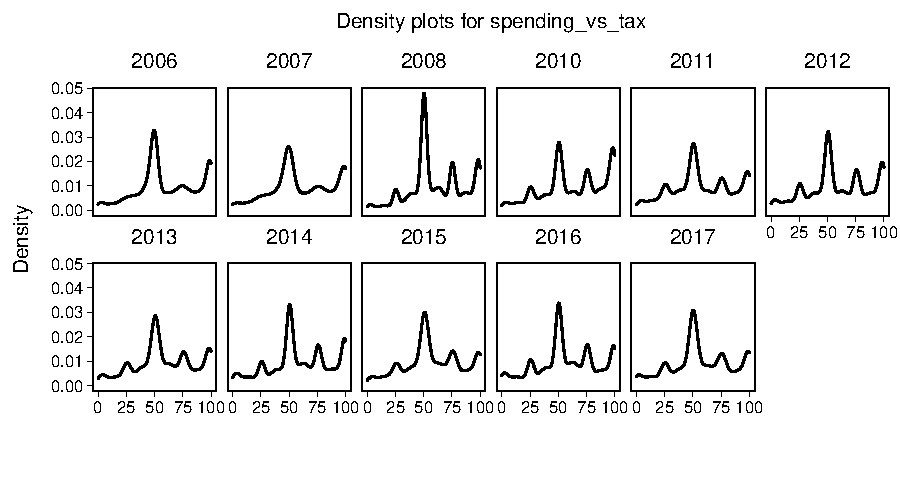
\includegraphics{guide_cumulative_ces_policy_preferences_files/figure-latex/unnamed-chunk-5-1} 

}

\caption{Density plots for question item}\label{fig:unnamed-chunk-5-1}
\end{figure}

Year-specific variable names and
wording\begingroup\fontsize{11}{13}\selectfont

\begin{longtable}[t]{rl>{\raggedright\arraybackslash}p{10cm}}
\caption{\label{tab:unnamed-chunk-5}spending\_vs\_tax: Year-specific wording}\\
\toprule
Year & Variable & Question wording\\
\midrule
\endfirsthead
\caption[]{spending\_vs\_tax: Year-specific wording \textit{(continued)}}\\
\toprule
Year & Variable & Question wording\\
\midrule
\endhead

\endfoot
\bottomrule
\endlastfoot
2006 & v4040 & If your state were to have a budget deficit this year it would have to raise taxes on income or sales or cut spending, such as on education, health care, welfare, and road construction. What would you prefer more raising taxes or cutting spending? Choose a point along the scale from 100 percent tax increases (and no spending cuts) to 100 percent spending cuts (and 0 percent no tax increases). The point in the middle means that any the budget should be balanced with equal amounts of spending cuts and tax increases.  If you are not sure, or don't know, please check here: [dk]\\
\addlinespace
2007 & CC06\_V4040 & If your state were to have a budget deficit this year it would have to raise taxes on income or sales or cut spending, such as on education, health care, welfare, and road construction. What would you prefer more raising taxes or cutting spending? Choose a point along the scale from 100 percent tax increases (and no spending cuts) to 100 percent spending cuts (and 0 percent no tax increases). The point in the middle means that any the budget should be balanced with equal amounts of spending cuts and tax increases.\\
\addlinespace
2008 & cc420 & If your state were to have a budget deficit this year it would have to raise taxes on income or sales or cut spending, such as on education, health care, welfare, and road construction. What would you prefer more, raising taxes or cutting spending? Choose a point along the scale from 100 percent tax increases (and no spending cuts) to 100 percent spending cuts (and no tax increases). The point in the middle means that the budget should be balanced with equal amounts of spending cuts and tax increases.  If you are not sure, or don't know, please check the box below... Values in range 0 to 100\\
\addlinespace
2010 & CC415r & If your state were to have a budget deficit this year it would have to raise taxes on income or sales or cut spending, such as on education, health care, welfare, and road construction. What would you prefer more, raising taxes or cutting spending? Choose a point along the scale from 100 percent tax increases (and no spending cuts) to 100 percent spending cuts (and no tax increases). The point in the middle means that the budget should be balanced with equal amounts of spending cuts and tax increases. If you are not sure, or don't know, please check the box below Values in range 0 to 100\\
\addlinespace
2011 & CC357 & Raise Taxes or Cut Spending Rule\\
\addlinespace
2012 & CC415r & If your state were to have a budget deficit this year it would have to raise taxes on income and sales or cut spending, such as on education, health care, welfare, and road construction. What would you prefer more raising taxes or cutting spending? Choose a point along the scale from 100 percent tax increases (and no spending cuts) to 100 percent spending cuts (and no tax increases). The point in the middle means that the budget should be balanced with equal amounts of spending cuts and tax increases. If you are Not sure, or don't know, please check the 'not sure' box.\\
\addlinespace
2013 & CC13\_323 & If your state were to have a budget deficit this year it would have to raise taxes on income and sales or cut spending, such as on education, health care, welfare, and road construction. What would you prefer more raising taxes or cutting spending? Choose a point along the scale from 100 percent tax increases (and no spending cuts) to 100 percent spending cuts (and no tax increases). The point in the middle means that the budget should be balanced with equal amounts of spending cuts and tax increases. If you are Not sure, or don't know, please check the 'not sure' box.\\
\addlinespace
2014 & CC415r & If your state were to have a budget deficit this year it would have to raise taxes on income and sales or cut spending, such as on education, health care, welfare, and road construction. What would you prefer more raising taxes or cutting spending? Choose a point along the scale from 100 percent tax increases (and no spending cuts) to 100 percent spending cuts (and no tax increases). The point in the middle means that the budget should be balanced with equal amounts of spending cuts and tax increases. If you are Not sure, or don't know, please check the 'not sure' box.\\
\addlinespace
2015 & CC15\_331 & If your state were to have a budget deficit this year it would have to raise taxes on income and sales or cut spending, such as on education, health care, welfare, and road construction. What would you prefer more raising taxes or cutting spending? Choose a point along the scale from 100 percent tax increases (and no spending cuts) to 100 percent spending cuts (and no tax increases). The point in the middle means that the budget should be balanced with equal amounts of spending cuts and tax increases. If you are Not sure, or don't know, please check the 'Not sure' box.\\
\addlinespace
2016 & CC16\_415r & If your state were to have a budget deficit this year it would have to raise taxes on income and sales or cut spending, such as on education, health care, welfare, and road construction. What would you prefer more, raising taxes or cutting spending? Choose a point along the scale from 100\\
\addlinespace
2017 & CC17\_343 & If your state were to have a budget deficit this year it would have to raise taxes on income and sales or cut spending, such as on education, health care, welfare, and road construction. What would you prefer more raising taxes or cutting spending? Choose a point along the scale from 100 percent tax increases (and no spending cuts) to 100 percent spending cuts (and no tax increases). The point in the middle means that the budget should be balanced with equal amounts of spending cuts and tax increases. If you are Not sure, or don't know, please check the 'Not sure' box.\\
\addlinespace
2020 & CC20\_421r & Tax increases vs. Spending cuts\\*
\end{longtable}
\endgroup{}

\hypertarget{spending_cuts_most}{%
\subsubsection{spending\_cuts\_most}\label{spending_cuts_most}}

Most preferred spending cut option (1=Defense, 2=Domestic, 3=Raise
taxes)

Years in data: 2006, 2007, 2008, 2010, 2011, 2012, 2013, 2014, 2015,
2017\begingroup\fontsize{10}{12}\selectfont

\begin{longtable}[t]{lcccc}
\caption{\label{tab:unnamed-chunk-5}spending\_cuts\_most: Frequency table}\\
\toprule
Year & Cut defense spending & Cut domestic spending & Raise taxes & Borrow\\
\midrule
\endfirsthead
\caption[]{spending\_cuts\_most: Frequency table \textit{(continued)}}\\
\toprule
Year & Cut defense spending & Cut domestic spending & Raise taxes & Borrow\\
\midrule
\endhead

\endfoot
\bottomrule
\endlastfoot
2006 & 9,310 & 14,579 & 4,813 & 1,396\\
2007 & 3,270 & 4,647 & 1,659 & 365\\
2008 & 12,282 & 17,183 & 3,150 & 0\\
2010 & 21,673 & 24,909 & 8,209 & 0\\
2011 & 7,227 & 7,538 & 5,385 & 0\\
2012 & 21,793 & 20,865 & 11,081 & 0\\
2013 & 7,182 & 5,794 & 3,219 & 0\\
2014 & 23,581 & 20,764 & 11,218 & 0\\
2015 & 5,525 & 5,552 & 2,940 & 0\\
2017 & 7,846 & 6,366 & 3,787 & 0\\*
\end{longtable}
\endgroup{}

Year-specific variable names and
wording\begingroup\fontsize{11}{13}\selectfont

\begin{longtable}[t]{rl>{\raggedright\arraybackslash}p{10cm}}
\caption{\label{tab:unnamed-chunk-5}spending\_cuts\_most: Year-specific wording}\\
\toprule
Year & Variable & Question wording\\
\midrule
\endfirsthead
\caption[]{spending\_cuts\_most: Year-specific wording \textit{(continued)}}\\
\toprule
Year & Variable & Question wording\\
\midrule
\endhead

\endfoot
\bottomrule
\endlastfoot
2006 & v4044 & What would you most prefer that Congress do - cut domestic spending, cut military spending, raise taxes, or borrow funds?\\
\addlinespace
2007 & CC06\_V4044 & What would you most prefer that Congress do - cut domestic spending, cut military spending, raise taxes, or borrow funds?\\
\addlinespace
2008 & cc309 & What would you most prefer that Congress do - cut domestic spending, cut military spending, or raise taxes?\\
\addlinespace
2010 & CC328 & The federal budget is approximately 600 billion this year. If the Congress were to balance the budget it would have to consider cutting defense spending, cutting domestic spending (such as Medicare or Social Security), or raising taxes to cover the deficit. What would you most prefer that Congress do - cut domestic spending, cut defense spending, or raise taxes?\\
\addlinespace
2011 & CC355a & Budget Balance 1\\
\addlinespace
2012 & CC328 & The federal budget deficit is approximately 1 trillion this year. If the Congress were to balance the budget it would have to consider cutting defense spending, cutting domestic spending (such as Medicare and Social Security), or raising taxes to cover the deficit. What would you MOST prefer that Congress do - cut domestic spending, cut defense spending, or raise taxes\\
\addlinespace
2013 & CC13\_331a & If your state were to have a budget deficit this year it would have to raise taxes on income and sales or cut spending, such as on education, health care, welfare, and road construction. What would you prefer more raising taxes or cutting spending? Choose a point along the scale from 100 percent tax increases (and no spending cuts) to 100 percent spending cuts (and no tax increases). The point in the middle means that the budget should be balanced with equal amounts of spending cuts and tax increases. If you are Not sure, or don't know, please check the 'not sure' box.\\
\addlinespace
2014 & CC14\_329a & The federal budget deficit is approximately 500 billion this year. If the Congress were to balance the budget it would have to consider cutting defense spending, cutting domestic spending (such as Medicare and Social Security), or raising taxes to cover the deficit. What would you most prefer that Congress do - cut domestic spending, cut defense spending, or raise taxes?\\
\addlinespace
2015 & CC15\_333a & The federal budget deficit is approximately 1 trillion this year. If the Congress were to balance the budget it would have to consider cutting defense spending, cutting domestic spending (such as Medicare and Social Security), or raising taxes to cover the deficit. What would you most prefer that Congress do - cut domestic spending, cut defense spending, or raise taxes?\\
\addlinespace
2017 & CC17\_345a & The federal budget deficit is approximately 700 billion this year. If the Congress were to balance the budget it would have to consider cutting defense spending, cutting domestic spending (such as Medicare and Social Security), or raising taxes to cover the deficit. What would you most prefer that Congress do - cut domestic spending, cut defense spending, or raise taxes?\\*
\end{longtable}
\endgroup{}

\emph{Note: In 2006 and 2007, this question includes a fourth response
option, `Borrow'.}

\hypertarget{spending_cuts_least}{%
\subsubsection{spending\_cuts\_least}\label{spending_cuts_least}}

Least preferred spending cut option (1=Defense, 2=Domestic, 3=Raise
taxes)

Years in data: 2006, 2007, 2008, 2010, 2011, 2012, 2013, 2014, 2015,
2017\begingroup\fontsize{10}{12}\selectfont

\begin{longtable}[t]{lcccc}
\caption{\label{tab:unnamed-chunk-5}spending\_cuts\_least: Frequency table}\\
\toprule
Year & Cut defense spending & Cut domestic spending & Raise taxes & Borrow\\
\midrule
\endfirsthead
\caption[]{spending\_cuts\_least: Frequency table \textit{(continued)}}\\
\toprule
Year & Cut defense spending & Cut domestic spending & Raise taxes & Borrow\\
\midrule
\endhead

\endfoot
\bottomrule
\endlastfoot
2006 & 6,891 & 3,257 & 7,942 & 11,064\\
2007 & 2,051 & 1,208 & 2,629 & 3,822\\
2008 & 6,212 & 7,270 & 19,198 & 0\\
2010 & 8,142 & 16,876 & 29,575 & 0\\
2011 & 4,721 & 7,445 & 7,801 & 0\\
2012 & 10,493 & 19,130 & 23,876 & 0\\
2013 & 2,665 & 6,131 & 7,343 & 0\\
2014 & 11,694 & 18,583 & 25,098 & 0\\
2015 & 3,232 & 4,939 & 5,917 & 0\\
2017 & 4,035 & 6,943 & 7,010 & 0\\*
\end{longtable}
\endgroup{}

Year-specific variable names and
wording\begingroup\fontsize{11}{13}\selectfont

\begin{longtable}[t]{rl>{\raggedright\arraybackslash}p{10cm}}
\caption{\label{tab:unnamed-chunk-5}spending\_cuts\_least: Year-specific wording}\\
\toprule
Year & Variable & Question wording\\
\midrule
\endfirsthead
\caption[]{spending\_cuts\_least: Year-specific wording \textit{(continued)}}\\
\toprule
Year & Variable & Question wording\\
\midrule
\endhead

\endfoot
\bottomrule
\endlastfoot
2006 & v4046 & What do you least want Congress to do?\\
\addlinespace
2007 & CC06\_V4046 & Should Congress cut spending, raise taxes, or borrow... What do you least want Congress to do?\\
\addlinespace
2008 & cc310a & What do you least want Congress to do?\\
\addlinespace
2010 & CC329 & The federal budget is approximately 600 billion this year. If the Congress were to balance the budget it would have to consider cutting defense spending, cutting domestic spending (such as Medicare or Social Security), or raising taxes to cover the deficit. What do you least want Congress to do?\\
\addlinespace
2011 & CC355b & Budget Balance 2\\
\addlinespace
2012 & CC329 & The federal budget deficit is approximately 1 trillion this year. If the Congress were to balance the budget it would have to consider cutting defense spending, cutting domestic spending (such as Medicare and Social Security), or raising taxes to cover the deficit. What would you LEAST prefer that Congress do - cut domestic spending, cut defense spending, or raise taxes\\
\addlinespace
2013 & CC13\_331b & If the state had to raise taxes, what share of the tax increase should come from increased income taxes and what share from increased sales taxes? Choose a point along the scale from 100 percent from sales (and none from income) to 100 percent from income (and none from sales). The point in the middle means that any increase in taxes should come equally from sales and income taxes. If you are Not sure, or don't know, please check the 'not sure' box.\\
\addlinespace
2014 & CC14\_329b & The federal budget deficit is approximately 500 billion this year. If the Congress were to balance the budget it would have to consider cutting defense spending, cutting domestic spending (such as Medicare and Social Security), or raising taxes to cover the deficit. What do you least want Congress to do?\\
\addlinespace
2015 & CC15\_333b & The federal budget deficit is approximately 1 trillion this year. If the Congress were to balance the budget it would have to consider cutting defense spending, cutting domestic spending (such as Medicare and Social Security), or raising taxes to cover the deficit. What do you least want Congress to do?\\
\addlinespace
2017 & CC17\_345b & The federal budget deficit is approximately 700 billion this year. If the Congress were to balance the budget it would have to consider cutting defense spending, cutting domestic spending (such as Medicare and Social Security), or raising taxes to cover the deficit. What do you least want Congress to do?\\*
\end{longtable}
\endgroup{}

\emph{Note: In 2006 and 2007, this question includes a fourth response
option, `Borrow'.}

\newpage

\hypertarget{trade}{%
\subsection{Trade}\label{trade}}

\hypertarget{trade_china}{%
\subsubsection{trade\_china}\label{trade_china}}

Tariffs on goods imported from China

Years in data: 2018, 2019, 2020,
2021\begingroup\fontsize{10}{12}\selectfont

\begin{longtable}[t]{lcccc}
\caption{\label{tab:unnamed-chunk-5}trade\_china: Frequency table}\\
\toprule
Response & 2018 & 2019 & 2020 & 2021\\
\midrule
\endfirsthead
\caption[]{trade\_china: Frequency table \textit{(continued)}}\\
\toprule
Response & 2018 & 2019 & 2020 & 2021\\
\midrule
\endhead

\endfoot
\bottomrule
\endlastfoot
Support & 29,290 & 9,128 & 35,793 & 16,081\\
Oppose & 30,591 & 8,573 & 24,633 & 9,601\\*
\end{longtable}
\endgroup{}

Year-specific variable names and
wording\begingroup\fontsize{11}{13}\selectfont

\begin{longtable}[t]{rl>{\raggedright\arraybackslash}p{10cm}}
\caption{\label{tab:unnamed-chunk-5}trade\_china: Year-specific wording}\\
\toprule
Year & Variable & Question wording\\
\midrule
\endfirsthead
\caption[]{trade\_china: Year-specific wording \textit{(continued)}}\\
\toprule
Year & Variable & Question wording\\
\midrule
\endhead

\endfoot
\bottomrule
\endlastfoot
2018 & CC18\_331a & Tariffs on 200 billion dollars worth of goods imported from China\\
\addlinespace
2019 & CC19\_331a & 20 percent tariffs on goods imported from China\\
\addlinespace
2020 & CC20\_338a & Tariffs on 200 billion dollars worth of goods imported from China\\
\addlinespace
2021 & CC21\_325a & 20 percent tariffs on goods imported from China\\*
\end{longtable}
\endgroup{}

\hypertarget{trade_canmex_except}{%
\subsubsection{trade\_canmex\_except}\label{trade_canmex_except}}

Tariffs on steel and aluminum EXCEPT from Canada and Mexico

Years in data: 2018, 2019, 2020\begingroup\fontsize{10}{12}\selectfont

\begin{longtable}[t]{lccc}
\caption{\label{tab:unnamed-chunk-5}trade\_canmex\_except: Frequency table}\\
\toprule
Response & 2018 & 2019 & 2020\\
\midrule
\endfirsthead
\caption[]{trade\_canmex\_except: Frequency table \textit{(continued)}}\\
\toprule
Response & 2018 & 2019 & 2020\\
\midrule
\endhead

\endfoot
\bottomrule
\endlastfoot
Support & 28,817 & 8,870 & 33,614\\
Oppose & 31,036 & 8,799 & 26,784\\*
\end{longtable}
\endgroup{}

Year-specific variable names and
wording\begingroup\fontsize{11}{13}\selectfont

\begin{longtable}[t]{rl>{\raggedright\arraybackslash}p{10cm}}
\caption{\label{tab:unnamed-chunk-5}trade\_canmex\_except: Year-specific wording}\\
\toprule
Year & Variable & Question wording\\
\midrule
\endfirsthead
\caption[]{trade\_canmex\_except: Year-specific wording \textit{(continued)}}\\
\toprule
Year & Variable & Question wording\\
\midrule
\endhead

\endfoot
\bottomrule
\endlastfoot
2018 & CC18\_331b & 25 percent tariffs on imported steel and 10percent on imported aluminum, EXCEPT from Canada and Mexico.\\
\addlinespace
2019 & CC19\_331b & 25 percent tariffs on imported steel and 10percent on imported aluminum, EXCEPT from Canada and Mexico.\\
\addlinespace
2020 & CC20\_338b & 25 percent tariffs on imported steel and 10percent on imported aluminum, EXCEPT from Canada and Mexico.\\*
\end{longtable}
\endgroup{}

\hypertarget{trade_canmex_include}{%
\subsubsection{trade\_canmex\_include}\label{trade_canmex_include}}

Tariffs on steel and aluminum INCLUDING from Canada and Mexico

Years in data: 2018, 2019, 2020,
2021\begingroup\fontsize{10}{12}\selectfont

\begin{longtable}[t]{lcccc}
\caption{\label{tab:unnamed-chunk-5}trade\_canmex\_include: Frequency table}\\
\toprule
Response & 2018 & 2019 & 2020 & 2021\\
\midrule
\endfirsthead
\caption[]{trade\_canmex\_include: Frequency table \textit{(continued)}}\\
\toprule
Response & 2018 & 2019 & 2020 & 2021\\
\midrule
\endhead

\endfoot
\bottomrule
\endlastfoot
Support & 21,137 & 5,929 & 20,920 & 14,582\\
Oppose & 38,738 & 11,706 & 39,349 & 11,099\\*
\end{longtable}
\endgroup{}

Year-specific variable names and
wording\begingroup\fontsize{11}{13}\selectfont

\begin{longtable}[t]{rl>{\raggedright\arraybackslash}p{10cm}}
\caption{\label{tab:unnamed-chunk-5}trade\_canmex\_include: Year-specific wording}\\
\toprule
Year & Variable & Question wording\\
\midrule
\endfirsthead
\caption[]{trade\_canmex\_include: Year-specific wording \textit{(continued)}}\\
\toprule
Year & Variable & Question wording\\
\midrule
\endhead

\endfoot
\bottomrule
\endlastfoot
2018 & CC18\_331c & 25 percent tariffs on all imported steel and 10percent on imported aluminum, INCLUDING from Canada and Mexico.\\
\addlinespace
2019 & CC19\_331c & 25 percent tariffs on imported steel and 10 percent on imported aluminum.\\
\addlinespace
2020 & CC20\_338c & 25 percent tariffs on all imported steel and 10percent on imported aluminum, INCLUDING from Canada and Mexico.\\
\addlinespace
2021 & CC21\_325b & 25 percent tariffs on imported steel and 10 percent on imported aluminum.\\*
\end{longtable}
\endgroup{}
\newpage

\hypertarget{other}{%
\subsection{Other}\label{other}}

\hypertarget{gaymarriage_scale}{%
\subsubsection{gaymarriage\_scale}\label{gaymarriage_scale}}

Opposition scale to gay marriage (1=Strongly support, 4=Strongly oppose)

Years in data: 2006, 2007\begingroup\fontsize{10}{12}\selectfont

\begin{longtable}[t]{lcc}
\caption{\label{tab:unnamed-chunk-5}gaymarriage\_scale: Frequency table}\\
\toprule
Response & 2006 & 2007\\
\midrule
\endfirsthead
\caption[]{gaymarriage\_scale: Frequency table \textit{(continued)}}\\
\toprule
Response & 2006 & 2007\\
\midrule
\endhead

\endfoot
\bottomrule
\endlastfoot
Strongly support & 5,848 & 1,958\\
Somewhat support & 1,571 & 529\\
Somewhat oppose & 1,462 & 506\\
Stongly oppose & 6,937 & 2,893\\
Don't know & 418 & 144\\*
\end{longtable}
\endgroup{}

Year-specific variable names and
wording\begingroup\fontsize{11}{13}\selectfont

\begin{longtable}[t]{rl>{\raggedright\arraybackslash}p{10cm}}
\caption{\label{tab:unnamed-chunk-5}gaymarriage\_scale: Year-specific wording}\\
\toprule
Year & Variable & Question wording\\
\midrule
\endfirsthead
\caption[]{gaymarriage\_scale: Year-specific wording \textit{(continued)}}\\
\toprule
Year & Variable & Question wording\\
\midrule
\endhead

\endfoot
\bottomrule
\endlastfoot
2006 & v2103 & President Bush recently spoke out in favor of a Constitutional Amendment defining marriage as strictly between a man and a woman. Do you support or oppose a Constitutional amendment banning gay marriage?\\
\addlinespace
2007 & CC06\_V2103 & President Bush recently spoke out in favor of a Constitutional Amendment defining marriage as strictly between a man and a woman. Do you support or oppose a Constitutional amendment banning gay marriage?\\*
\end{longtable}
\endgroup{}

\hypertarget{gaymarriage_ban}{%
\subsubsection{gaymarriage\_ban}\label{gaymarriage_ban}}

Amendment banning gay marriage

Years in data: 2008, 2009, 2010,
2011\begingroup\fontsize{10}{12}\selectfont

\begin{longtable}[t]{lcccc}
\caption{\label{tab:unnamed-chunk-5}gaymarriage\_ban: Frequency table}\\
\toprule
Response & 2008 & 2009 & 2010 & 2011\\
\midrule
\endfirsthead
\caption[]{gaymarriage\_ban: Frequency table \textit{(continued)}}\\
\toprule
Response & 2008 & 2009 & 2010 & 2011\\
\midrule
\endhead

\endfoot
\bottomrule
\endlastfoot
Support & 13,730 & 6,067 & 23,586 & 7,942\\
Oppose & 15,216 & 7,674 & 31,569 & 12,208\\*
\end{longtable}
\endgroup{}

Year-specific variable names and
wording\begingroup\fontsize{11}{13}\selectfont

\begin{longtable}[t]{rl>{\raggedright\arraybackslash}p{10cm}}
\caption{\label{tab:unnamed-chunk-5}gaymarriage\_ban: Year-specific wording}\\
\toprule
Year & Variable & Question wording\\
\midrule
\endfirsthead
\caption[]{gaymarriage\_ban: Year-specific wording \textit{(continued)}}\\
\toprule
Year & Variable & Question wording\\
\midrule
\endhead

\endfoot
\bottomrule
\endlastfoot
2008 & cc316f & Constitutional Amendment banning Gay Marriage\\
\addlinespace
2009 & cc09\_54 & Gay Marriage\\
\addlinespace
2010 & CC326 & Do you support a Constitutional Amendment banning Gay Marriage?\\
\addlinespace
2011 & CC353 & Gay Marriage\\*
\end{longtable}
\endgroup{}

\hypertarget{gaymarriage_legalize}{%
\subsubsection{gaymarriage\_legalize}\label{gaymarriage_legalize}}

Support for legalizing gay marriage

Years in data: 2012, 2013, 2014, 2015,
2016\begingroup\fontsize{10}{12}\selectfont

\begin{longtable}[t]{lccccc}
\caption{\label{tab:unnamed-chunk-5}gaymarriage\_legalize: Frequency table}\\
\toprule
Response & 2012 & 2013 & 2014 & 2015 & 2016\\
\midrule
\endfirsthead
\caption[]{gaymarriage\_legalize: Frequency table \textit{(continued)}}\\
\toprule
Response & 2012 & 2013 & 2014 & 2015 & 2016\\
\midrule
\endhead

\endfoot
\bottomrule
\endlastfoot
Support & 28,085 & 9,308 & 32,810 & 8,248 & 41,718\\
Oppose & 25,857 & 6,867 & 22,860 & 5,841 & 22,407\\*
\end{longtable}
\endgroup{}

Year-specific variable names and
wording\begingroup\fontsize{11}{13}\selectfont

\begin{longtable}[t]{rl>{\raggedright\arraybackslash}p{10cm}}
\caption{\label{tab:unnamed-chunk-5}gaymarriage\_legalize: Year-specific wording}\\
\toprule
Year & Variable & Question wording\\
\midrule
\endfirsthead
\caption[]{gaymarriage\_legalize: Year-specific wording \textit{(continued)}}\\
\toprule
Year & Variable & Question wording\\
\midrule
\endhead

\endfoot
\bottomrule
\endlastfoot
2012 & CC326 & Do you favor or oppose allowing gays and lesbians to marry legally?\\
\addlinespace
2013 & CC329 & Do you favor or oppose allowing gays and lesbians to marry legally?\\
\addlinespace
2014 & CC14\_327 & Do you favor or oppose allowing gays and lesbians to marry legally?\\
\addlinespace
2015 & CC15\_325 & Do you favor or oppose allowing gays and lesbians to marry legally?\\
\addlinespace
2016 & CC16\_335 & Do you favor or oppose allowing gays and lesbians to marry legally?\\*
\end{longtable}
\endgroup{}

\hypertarget{affirmativeaction_scale}{%
\subsubsection{affirmativeaction\_scale}\label{affirmativeaction_scale}}

Opposition scale to affirmative action (1 = Strongly support, 7 =
Strongly oppose)

Years in data: 2006, 2007\begingroup\fontsize{10}{12}\selectfont

\begin{longtable}[t]{lcc}
\caption{\label{tab:unnamed-chunk-5}affirmativeaction\_scale: Frequency table}\\
\toprule
Response & 2006 & 2007\\
\midrule
\endfirsthead
\caption[]{affirmativeaction\_scale: Frequency table \textit{(continued)}}\\
\toprule
Response & 2006 & 2007\\
\midrule
\endhead

\endfoot
\bottomrule
\endlastfoot
Strongly support & 4,503 & 1,030\\
Support & 3,571 & 1,069\\
Somewhat support & 3,839 & 1,185\\
Neither support nor oppose & 6,630 & 1,726\\
Somewhat oppose & 3,152 & 839\\
Oppose & 3,909 & 1,125\\
Strongly oppose & 10,662 & 2,999\\*
\end{longtable}
\endgroup{}

Year-specific variable names and
wording\begingroup\fontsize{11}{13}\selectfont

\begin{longtable}[t]{rl>{\raggedright\arraybackslash}p{10cm}}
\caption{\label{tab:unnamed-chunk-5}affirmativeaction\_scale: Year-specific wording}\\
\toprule
Year & Variable & Question wording\\
\midrule
\endfirsthead
\caption[]{affirmativeaction\_scale: Year-specific wording \textit{(continued)}}\\
\toprule
Year & Variable & Question wording\\
\midrule
\endhead

\endfoot
\bottomrule
\endlastfoot
2006 & v3027 & Some people think that if a company has a history of discriminating against blacks when making hiring decisions, then they should be required to have an affirmative action program that gives blacks preference in hiring.    What do you think? Should companies that have discriminated against blacks have to have an affirmative action program?\\
\addlinespace
2007 & CC06\_V3027 & Some people think that if a company has a history of discriminating against blacks when making hiring decisions, then they should be required to have an affirmative action program that gives blacks preference in hiring. What do you think? Should companies that have discriminated against blacks have to have an affirmative action program?\\*
\end{longtable}
\endgroup{}

\emph{Note: In 2006 and 2007, this question includes a fourth response
option, `Not sure', which has been re-coded as `NA' in this data set.}

\hypertarget{affirmativeaction}{%
\subsubsection{affirmativeaction}\label{affirmativeaction}}

Opposition to affirmative action (1 = Support, 4 = Oppose)

Years in data: 2008, 2009, 2010, 2011, 2012, 2013,
2014\begingroup\fontsize{10}{12}\selectfont

\begin{longtable}[t]{lccccccc}
\caption{\label{tab:unnamed-chunk-5}affirmativeaction: Frequency table}\\
\toprule
Response & 2008 & 2009 & 2010 & 2011 & 2012 & 2013 & 2014\\
\midrule
\endfirsthead
\caption[]{affirmativeaction: Frequency table \textit{(continued)}}\\
\toprule
Response & 2008 & 2009 & 2010 & 2011 & 2012 & 2013 & 2014\\
\midrule
\endhead

\endfoot
\bottomrule
\endlastfoot
Strongly support & 4,514 & 1,581 & 6,142 & 2,251 & 7,448 & 1,993 & 8,116\\
Somewhat support & 9,155 & 3,236 & 12,652 & 4,886 & 13,797 & 4,176 & 14,161\\
Somewhat oppose & 8,032 & 3,392 & 13,503 & 5,407 & 14,183 & 4,219 & 14,135\\
Strongly oppose & 10,912 & 5,541 & 22,974 & 7,579 & 18,869 & 5,930 & 19,591\\*
\end{longtable}
\endgroup{}

Year-specific variable names and
wording\begingroup\fontsize{11}{13}\selectfont

\begin{longtable}[t]{rl>{\raggedright\arraybackslash}p{10cm}}
\caption{\label{tab:unnamed-chunk-5}affirmativeaction: Year-specific wording}\\
\toprule
Year & Variable & Question wording\\
\midrule
\endfirsthead
\caption[]{affirmativeaction: Year-specific wording \textit{(continued)}}\\
\toprule
Year & Variable & Question wording\\
\midrule
\endhead

\endfoot
\bottomrule
\endlastfoot
2008 & cc313 & Affirmative action programs give preference to racial minorities and to women in employment and college admissions in order to correct for discrimination. Do you support or oppose affirmative action?\\
\addlinespace
2009 & cc09\_55 & Affirmative Action\\
\addlinespace
2010 & CC327 & Affirmative action programs give preference to racial minorities in employment and college admissions in order to correct for past discrimination. Do you support or oppose affirmative action?\\
\addlinespace
2011 & CC354 & Affirmative Action\\
\addlinespace
2012 & CC327 & Affirmative action programs give preference to racial minorities in employment and college admissions in order to correct for past discrimination. Do you support or oppose affirmative action?\\
\addlinespace
2013 & CC330 & Affirmative action programs give preference to racial minorities in employment and college admissions in order to correct for past discrimination. Do you support or oppose affirmative action?\\
\addlinespace
2014 & CC14\_328 & Affirmative action programs give preference to racial minorities in employment and college admissions in order to correct for past discrimination. Do you support or oppose affirmative action?\\*
\end{longtable}
\endgroup{}

\hypertarget{incometax_vs_salestax}{%
\subsubsection{incometax\_vs\_salestax}\label{incometax_vs_salestax}}

Preference scale from 0 (increase income tax) to 100 (increase sales
tax)

Years in data: 2006, 2007, 2008, 2010, 2011, 2012, 2013, 2014, 2015,
2016, 2017, 2020

\begin{figure}

{\centering 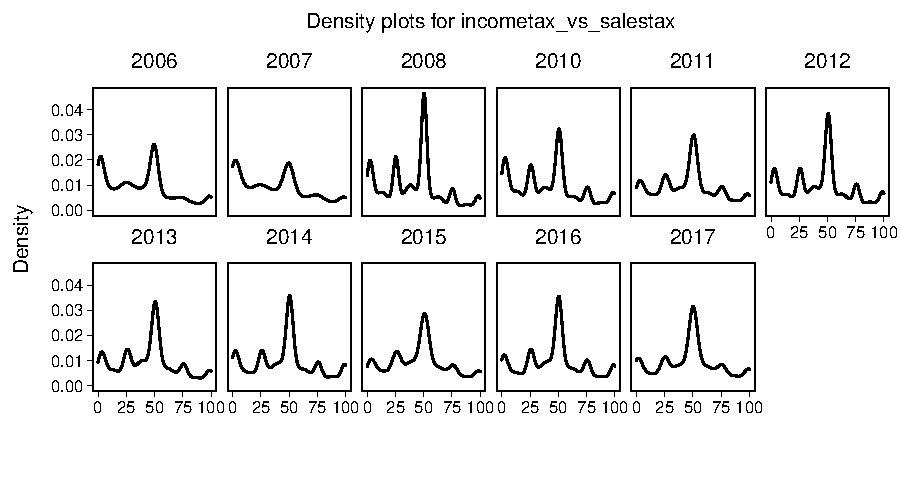
\includegraphics{guide_cumulative_ces_policy_preferences_files/figure-latex/unnamed-chunk-5-2} 

}

\caption{Density plots for question item}\label{fig:unnamed-chunk-5-2}
\end{figure}

Year-specific variable names and
wording\begingroup\fontsize{11}{13}\selectfont

\begin{longtable}[t]{rl>{\raggedright\arraybackslash}p{10cm}}
\caption{\label{tab:unnamed-chunk-5}incometax\_vs\_salestax: Year-specific wording}\\
\toprule
Year & Variable & Question wording\\
\midrule
\endfirsthead
\caption[]{incometax\_vs\_salestax: Year-specific wording \textit{(continued)}}\\
\toprule
Year & Variable & Question wording\\
\midrule
\endhead

\endfoot
\bottomrule
\endlastfoot
2006 & v4042 & If the state had to raise taxes, which taxes should it increase? Suppose that your state government has to raise some combination of sales taxes and individual income taxes in the coming year. What share of the tax increase should come from increased income taxes and what share from increased sales taxes? Choose a point along the scale from 100 percent from sales (and none from income) to 100 percent from income (and none from sales). The point in the middle means that any increase in taxes should come equally from sales and income taxes.  If you are not sure, or don't know, please check here: [dk]\\
\addlinespace
2007 & CC06\_V4042 & If the state had to raise taxes, which taxes should it increase? Suppose that your state government has to raise some combination of sales taxes and individual income taxes in the coming year. What share of the tax increase should come from increased income taxes and what share from increased sales taxes? Choose a point along the scale from 100 percent from sales (and none from income) to 100 percent from income (and none from sales). The point in the middle means that any increase in taxes should come equally from sales and income taxes.\\
\addlinespace
2008 & cc421 & If the state had to raise taxes, what share of the tax increase should come from increased income taxes and what share from increased sales taxes? Choose a point along the scale from 100 percent from sales (and none from income) to 100 percent from income (and none from sales). The point in the middle means that any increase in taxes should come equally from sales and income taxes.  If you are not sure, or don't know, please check the box below... Values in range 0 to 100\\
\addlinespace
2010 & CC416r & If the state had to raise taxes, what share of the tax increase should come from increased income taxes and what share from increased sales taxes? Choose a point along the scale from 100 percent from sales (and none from income) to 100 percent from income (and none from sales). The point in the middle means that any increase in taxes should come equally from sales and income taxes. If you are not sure, or don't know, please check the box below Values in range 0 to 100\\
\addlinespace
2011 & CC358 & Income vs Sales Tax Rule\\
\addlinespace
2012 & CC416r & If the state had to raise taxes, what share of the tax increase should come from increased income taxes and what share from increased sales taxes? Choose a point along the scale from 100 percent from sales (and none from income) to 100 percent from income (and none from sales). The point in the middle means that any increase in taxes should come equally from sales and income taxes. If you are Not sure, or don't know, please check the 'not sure' box.\\
\addlinespace
2013 & CC13\_324 & If the state had to raise taxes, what share of the tax increase should come from increased income taxes and what share from increased sales taxes? Choose a point along the scale from 100 percent from sales (and none from income) to 100 percent from income (and none from sales). The point in the middle means that any increase in taxes should come equally from sales and income taxes. If you are Not sure, or don't know, please check the 'not sure' box.\\
\addlinespace
2014 & CC416r & If the state had to raise taxes, what share of the tax increase should come from increased income taxes and what share from increased sales taxes? Choose a point along the scale from 100 percent from sales (and none from income) to 100 percent from income (and none from sales). The point in the middle means that any increase in taxes should come equally from sales and income taxes. If you are Not sure, or don't know, please check the 'not sure' box.\\
\addlinespace
2015 & CC15\_332 & If the state had to raise taxes, what share of the tax increase should come from increased income taxes and what share from increased sales taxes? Choose a point along the scale from 100 percent from sales (and none from income) to 100 percent from income (and none from sales). The point in the middle means that any increase in taxes should come equally from sales and income taxes. If you are Not sure, or don't know, please check the 'Not sure' box.\\
\addlinespace
2016 & CC16\_416r & If the state had to raise taxes, what share of the tax increase should come from increased income taxes and what share from increased sales taxes? Choose a point along the scale from 100\\
\addlinespace
2017 & CC17\_344 & If the state had to raise taxes, what share of the tax increase should come from increased income taxes and what share from increased sales taxes? Choose a point along the scale from 100 percent from sales (and none from income) to 100 percent from income (and none from sales). The point in the middle means that any increase in taxes should come equally from sales and income taxes. If you are Not sure, or don't know, please check the 'Not sure' box.\\
\addlinespace
2020 & CC20\_422r & Raise sales tax vs. Raise income tax\\*
\end{longtable}
\endgroup{}

\end{document}
